\documentclass[9pt,aspectratio=169]{beamer}

\usetheme{Madrid}
\usecolortheme{default}
\usefonttheme{professionalfonts}

\setbeamertemplate{navigation symbols}{}
\setbeamertemplate{footline}[frame number]
\setbeamercolor{block title}{bg=blue!20,fg=black}
\setbeamercolor{block body}{bg=blue!5,fg=black}

\usepackage[utf8]{inputenc}
\usepackage{amsmath}
\usepackage{booktabs}
\usepackage{array}
\usepackage{graphicx}
\usepackage{adjustbox}
\usepackage[most]{tcolorbox}
\usepackage{tikz}
\usetikzlibrary{arrows.meta,positioning,shapes.geometric}

\title[MyHealthReport V1]{MyHealthReport}
\subtitle{Version 1 Framework --- Expanded Edition\\ \small Motivation $\cdot$ Method $\cdot$ Result $\cdot$ Conclusion, with schematics for every module}
\author{}
\date{22 August 2026}

\begin{document}

\begin{frame}
\titlepage
\end{frame}

\begin{frame}{Agenda}
\tiny
\tableofcontents
\end{frame}

\section{Purpose \& Principles}

\begin{frame}{1. Purpose of Version 1}
\begin{columns}[T,onlytextwidth]
\begin{column}{0.5\textwidth}
\begin{tcolorbox}[colback=blue!7,colframe=blue!55!black,title=\textbf{Motivation},boxrule=0.6pt,arc=1mm,left=5pt,right=5pt,top=3pt,bottom=3pt,fonttitle=\small]
\footnotesize Users receive raw lab numbers with no structured way to understand, prioritise, or act on them.
\end{tcolorbox}
\vspace{5pt}
\begin{tcolorbox}[colback=teal!7,colframe=teal!55!black,title=\textbf{Method},boxrule=0.6pt,arc=1mm,left=5pt,right=5pt,top=3pt,bottom=3pt,fonttitle=\small]
\footnotesize Define nine sequential user-facing objectives, from profile through follow-up, without attempting independent diagnosis.
\end{tcolorbox}
\end{column}
\begin{column}{0.5\textwidth}
\begin{tcolorbox}[colback=green!8,colframe=green!45!black,title=\textbf{Result},boxrule=0.6pt,arc=1mm,left=5pt,right=5pt,top=3pt,bottom=3pt,fonttitle=\small]
\footnotesize A platform scope statement: interpret, prioritise, explain and track -- not diagnose.
\end{tcolorbox}
\vspace{5pt}
\begin{tcolorbox}[colback=orange!10,colframe=orange!65!black,title=\textbf{Conclusion},boxrule=0.6pt,arc=1mm,left=5pt,right=5pt,top=3pt,bottom=3pt,fonttitle=\small]
\footnotesize The Central Logic chain (Data $\to$ ... $\to$ Follow-up) is the single sentence Version 1 is built to deliver.
\end{tcolorbox}
\end{column}
\end{columns}
\end{frame}

\begin{frame}{1. Purpose of Version 1}
\textcolor{black!55}{\scriptsize The Central Logic, as a flowchart with keywords}\\[2pt]
\begin{center}
\begin{adjustbox}{max width=0.96\linewidth,max height=0.66\textheight}
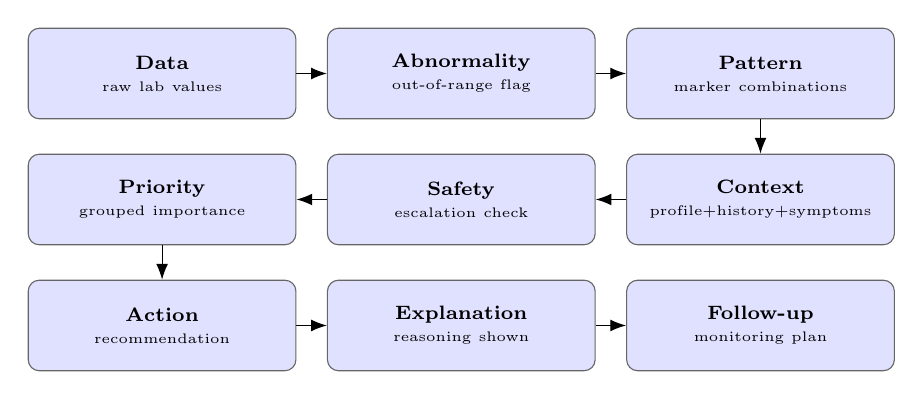
\begin{tikzpicture}[>=Latex]
\node[draw=black!60,rounded corners,fill=blue!12,minimum width=3.4cm,minimum height=1.15cm,align=center,font=\scriptsize,text width=3.15cm,inner sep=2pt] (s0) at (0.0,0.0) {\textbf{Data}\\\tiny raw lab values};
\node[draw=black!60,rounded corners,fill=blue!12,minimum width=3.4cm,minimum height=1.15cm,align=center,font=\scriptsize,text width=3.15cm,inner sep=2pt] (s1) at (3.8,0.0) {\textbf{Abnormality}\\\tiny out-of-range flag};
\node[draw=black!60,rounded corners,fill=blue!12,minimum width=3.4cm,minimum height=1.15cm,align=center,font=\scriptsize,text width=3.15cm,inner sep=2pt] (s2) at (7.6,0.0) {\textbf{Pattern}\\\tiny marker combinations};
\node[draw=black!60,rounded corners,fill=blue!12,minimum width=3.4cm,minimum height=1.15cm,align=center,font=\scriptsize,text width=3.15cm,inner sep=2pt] (s3) at (7.6,-1.5999999999999999) {\textbf{Context}\\\tiny profile+history+symptoms};
\node[draw=black!60,rounded corners,fill=blue!12,minimum width=3.4cm,minimum height=1.15cm,align=center,font=\scriptsize,text width=3.15cm,inner sep=2pt] (s4) at (3.8,-1.5999999999999999) {\textbf{Safety}\\\tiny escalation check};
\node[draw=black!60,rounded corners,fill=blue!12,minimum width=3.4cm,minimum height=1.15cm,align=center,font=\scriptsize,text width=3.15cm,inner sep=2pt] (s5) at (0.0,-1.5999999999999999) {\textbf{Priority}\\\tiny grouped importance};
\node[draw=black!60,rounded corners,fill=blue!12,minimum width=3.4cm,minimum height=1.15cm,align=center,font=\scriptsize,text width=3.15cm,inner sep=2pt] (s6) at (0.0,-3.1999999999999997) {\textbf{Action}\\\tiny recommendation};
\node[draw=black!60,rounded corners,fill=blue!12,minimum width=3.4cm,minimum height=1.15cm,align=center,font=\scriptsize,text width=3.15cm,inner sep=2pt] (s7) at (3.8,-3.1999999999999997) {\textbf{Explanation}\\\tiny reasoning shown};
\node[draw=black!60,rounded corners,fill=blue!12,minimum width=3.4cm,minimum height=1.15cm,align=center,font=\scriptsize,text width=3.15cm,inner sep=2pt] (s8) at (7.6,-3.1999999999999997) {\textbf{Follow-up}\\\tiny monitoring plan};
\draw[-{Latex[length=2mm]}] (s0.east)--(s1.west);
\draw[-{Latex[length=2mm]}] (s1.east)--(s2.west);
\draw[-{Latex[length=2mm]}] (s2.south)--(s3.north);
\draw[-{Latex[length=2mm]}] (s3.west)--(s4.east);
\draw[-{Latex[length=2mm]}] (s4.west)--(s5.east);
\draw[-{Latex[length=2mm]}] (s5.south)--(s6.north);
\draw[-{Latex[length=2mm]}] (s6.east)--(s7.west);
\draw[-{Latex[length=2mm]}] (s7.east)--(s8.west);
\end{tikzpicture}
\end{adjustbox}
\end{center}
\end{frame}

\begin{frame}{2. Core Design Principles}
\begin{columns}[T,onlytextwidth]
\begin{column}{0.5\textwidth}
\begin{tcolorbox}[colback=blue!7,colframe=blue!55!black,title=\textbf{Motivation},boxrule=0.6pt,arc=1mm,left=5pt,right=5pt,top=3pt,bottom=3pt,fonttitle=\small]
\footnotesize Without guiding principles, feature decisions drift toward complexity and clinical overreach.
\end{tcolorbox}
\vspace{5pt}
\begin{tcolorbox}[colback=teal!7,colframe=teal!55!black,title=\textbf{Method},boxrule=0.6pt,arc=1mm,left=5pt,right=5pt,top=3pt,bottom=3pt,fonttitle=\small]
\footnotesize Define five constraints spanning intake, interpretation, safety, transparency and prioritisation.
\end{tcolorbox}
\end{column}
\begin{column}{0.5\textwidth}
\begin{tcolorbox}[colback=green!8,colframe=green!45!black,title=\textbf{Result},boxrule=0.6pt,arc=1mm,left=5pt,right=5pt,top=3pt,bottom=3pt,fonttitle=\small]
\footnotesize Five testable rules every later module must satisfy.
\end{tcolorbox}
\vspace{5pt}
\begin{tcolorbox}[colback=orange!10,colframe=orange!65!black,title=\textbf{Conclusion},boxrule=0.6pt,arc=1mm,left=5pt,right=5pt,top=3pt,bottom=3pt,fonttitle=\small]
\footnotesize These principles are the filter every subsequent design decision passes through.
\end{tcolorbox}
\end{column}
\end{columns}
\end{frame}

\begin{frame}{2. Core Design Principles}
\textcolor{black!55}{\scriptsize Five constraints radiating from one design philosophy}\\[2pt]
\begin{center}
\begin{adjustbox}{max width=0.96\linewidth,max height=0.66\textheight}
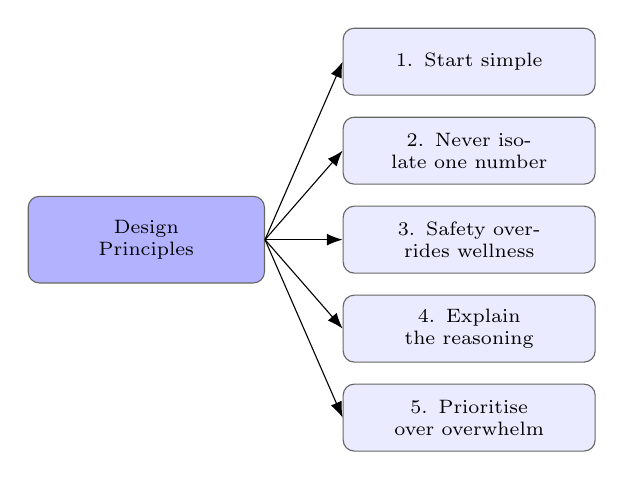
\begin{tikzpicture}[>=Latex]
\node[draw=black!60,rounded corners,fill=blue!30,minimum width=3.0cm,minimum height=1.1cm,align=center,font=\scriptsize,text width=2.75cm,inner sep=2pt] (cc) at (0,-2.2600000000000002) {Design\\Principles};
\node[draw=black!60,rounded corners,fill=blue!8,minimum width=3.2cm,minimum height=0.85cm,align=center,font=\scriptsize,text width=2.95cm,inner sep=2pt] (sp0) at (4.1,0) {1. Start simple};
\draw[-{Latex[length=2mm]}] (cc.east)--(sp0.west);
\node[draw=black!60,rounded corners,fill=blue!8,minimum width=3.2cm,minimum height=0.85cm,align=center,font=\scriptsize,text width=2.95cm,inner sep=2pt] (sp1) at (4.1,-1.13) {2. Never isolate one number};
\draw[-{Latex[length=2mm]}] (cc.east)--(sp1.west);
\node[draw=black!60,rounded corners,fill=blue!8,minimum width=3.2cm,minimum height=0.85cm,align=center,font=\scriptsize,text width=2.95cm,inner sep=2pt] (sp2) at (4.1,-2.26) {3. Safety overrides wellness};
\draw[-{Latex[length=2mm]}] (cc.east)--(sp2.west);
\node[draw=black!60,rounded corners,fill=blue!8,minimum width=3.2cm,minimum height=0.85cm,align=center,font=\scriptsize,text width=2.95cm,inner sep=2pt] (sp3) at (4.1,-3.3899999999999997) {4. Explain the reasoning};
\draw[-{Latex[length=2mm]}] (cc.east)--(sp3.west);
\node[draw=black!60,rounded corners,fill=blue!8,minimum width=3.2cm,minimum height=0.85cm,align=center,font=\scriptsize,text width=2.95cm,inner sep=2pt] (sp4) at (4.1,-4.52) {5. Prioritise over overwhelm};
\draw[-{Latex[length=2mm]}] (cc.east)--(sp4.west);
\end{tikzpicture}
\end{adjustbox}
\end{center}
\end{frame}

\section{System Architecture}

\begin{frame}{3. Version 1 System Architecture}
\begin{columns}[T,onlytextwidth]
\begin{column}{0.5\textwidth}
\begin{tcolorbox}[colback=blue!7,colframe=blue!55!black,title=\textbf{Motivation},boxrule=0.6pt,arc=1mm,left=5pt,right=5pt,top=3pt,bottom=3pt,fonttitle=\small]
\footnotesize A 20-module system needs one map showing how every piece connects before any module is built.
\end{tcolorbox}
\vspace{5pt}
\begin{tcolorbox}[colback=teal!7,colframe=teal!55!black,title=\textbf{Method},boxrule=0.6pt,arc=1mm,left=5pt,right=5pt,top=3pt,bottom=3pt,fonttitle=\small]
\footnotesize Lay out the full pipeline from registration to trend analysis, then group it by module cluster (macro) and trace it stage-by-stage (micro).
\end{tcolorbox}
\end{column}
\begin{column}{0.5\textwidth}
\begin{tcolorbox}[colback=green!8,colframe=green!45!black,title=\textbf{Result},boxrule=0.6pt,arc=1mm,left=5pt,right=5pt,top=3pt,bottom=3pt,fonttitle=\small]
\footnotesize A macro structure of 7 functional clusters, and a micro structure of 22 concrete pipeline stages tagged by module.
\end{tcolorbox}
\vspace{5pt}
\begin{tcolorbox}[colback=orange!10,colframe=orange!65!black,title=\textbf{Conclusion},boxrule=0.6pt,arc=1mm,left=5pt,right=5pt,top=3pt,bottom=3pt,fonttitle=\small]
\footnotesize Macro shows \textit{why} modules are grouped; micro shows \textit{exactly} how data moves between them.
\end{tcolorbox}
\end{column}
\end{columns}
\end{frame}

\begin{frame}{3. Version 1 System Architecture}
\textcolor{black!55}{\scriptsize Macro structure -- 7 clusters, module ranges, cluster-to-cluster flow}\\[2pt]
\begin{center}
\begin{adjustbox}{max width=0.96\linewidth,max height=0.66\textheight}
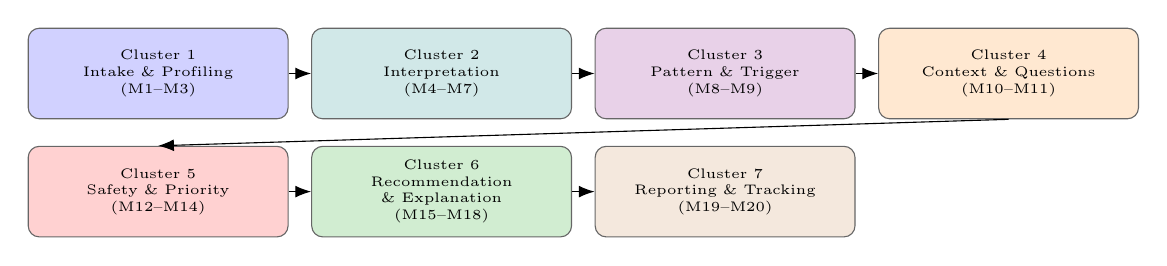
\begin{tikzpicture}[>=Latex]
\node[draw=black!60,rounded corners,fill=blue!18,minimum width=3.3cm,minimum height=1.15cm,align=center,font=\tiny,text width=3.05cm,inner sep=2pt] (mc0) at (0.0,0.0) {Cluster 1\\Intake \& Profiling\\(M1--M3)};
\node[draw=black!60,rounded corners,fill=teal!18,minimum width=3.3cm,minimum height=1.15cm,align=center,font=\tiny,text width=3.05cm,inner sep=2pt] (mc1) at (3.6,0.0) {Cluster 2\\Interpretation\\(M4--M7)};
\node[draw=black!60,rounded corners,fill=violet!18,minimum width=3.3cm,minimum height=1.15cm,align=center,font=\tiny,text width=3.05cm,inner sep=2pt] (mc2) at (7.2,0.0) {Cluster 3\\Pattern \& Trigger\\(M8--M9)};
\node[draw=black!60,rounded corners,fill=orange!18,minimum width=3.3cm,minimum height=1.15cm,align=center,font=\tiny,text width=3.05cm,inner sep=2pt] (mc3) at (10.8,0.0) {Cluster 4\\Context \& Questions\\(M10--M11)};
\node[draw=black!60,rounded corners,fill=red!18,minimum width=3.3cm,minimum height=1.15cm,align=center,font=\tiny,text width=3.05cm,inner sep=2pt] (mc4) at (0.0,-1.5) {Cluster 5\\Safety \& Priority\\(M12--M14)};
\node[draw=black!60,rounded corners,fill=green!60!black!18,minimum width=3.3cm,minimum height=1.15cm,align=center,font=\tiny,text width=3.05cm,inner sep=2pt] (mc5) at (3.6,-1.5) {Cluster 6\\Recommendation \& Explanation\\(M15--M18)};
\node[draw=black!60,rounded corners,fill=brown!18,minimum width=3.3cm,minimum height=1.15cm,align=center,font=\tiny,text width=3.05cm,inner sep=2pt] (mc6) at (7.2,-1.5) {Cluster 7\\Reporting \& Tracking\\(M19--M20)};
\draw[-{Latex[length=2mm]}] (mc0.east)--(mc1.west);
\draw[-{Latex[length=2mm]}] (mc1.east)--(mc2.west);
\draw[-{Latex[length=2mm]}] (mc2.east)--(mc3.west);
\draw[-{Latex[length=2mm]}] (mc3.south)--(mc4.north);
\draw[-{Latex[length=2mm]}] (mc4.east)--(mc5.west);
\draw[-{Latex[length=2mm]}] (mc5.east)--(mc6.west);
\end{tikzpicture}
\end{adjustbox}
\end{center}
\end{frame}

\begin{frame}{3. Version 1 System Architecture}
\textcolor{black!55}{\scriptsize Micro structure -- 22 pipeline stages, each tagged by its module/cluster}\\[2pt]
\begin{center}
\begin{adjustbox}{max width=0.96\linewidth,max height=0.66\textheight}
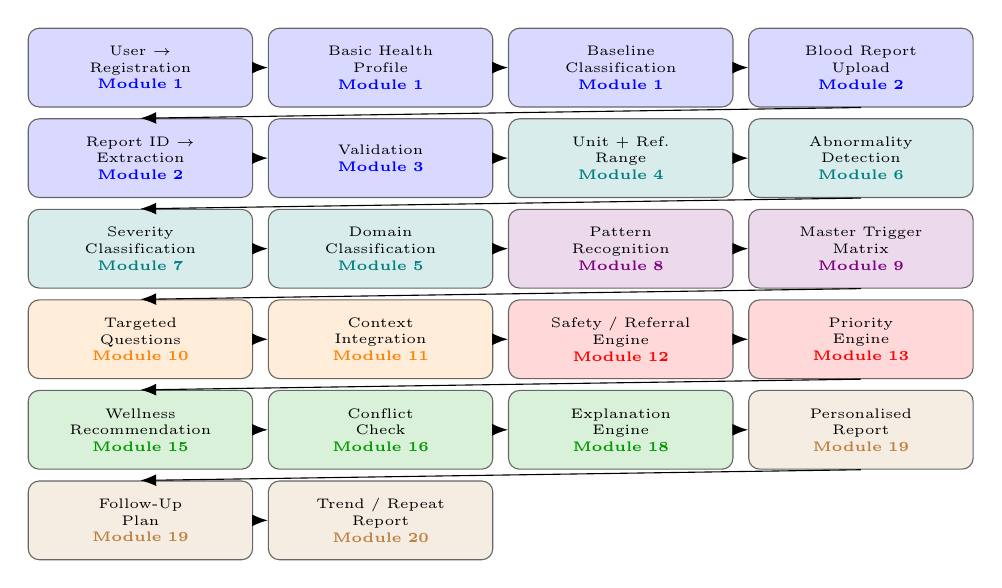
\begin{tikzpicture}[>=Latex]
\node[draw=black!60,rounded corners,fill=blue!15,minimum width=2.85cm,minimum height=1.0cm,align=center,font=\tiny,text width=2.6cm,inner sep=2pt] (mi0) at (0.0,0.0) {User $\to$\\Registration\\{\tiny\textcolor{blue}{\textbf{Module 1}}}};
\node[draw=black!60,rounded corners,fill=blue!15,minimum width=2.85cm,minimum height=1.0cm,align=center,font=\tiny,text width=2.6cm,inner sep=2pt] (mi1) at (3.05,0.0) {Basic Health\\Profile\\{\tiny\textcolor{blue}{\textbf{Module 1}}}};
\node[draw=black!60,rounded corners,fill=blue!15,minimum width=2.85cm,minimum height=1.0cm,align=center,font=\tiny,text width=2.6cm,inner sep=2pt] (mi2) at (6.1,0.0) {Baseline\\Classification\\{\tiny\textcolor{blue}{\textbf{Module 1}}}};
\node[draw=black!60,rounded corners,fill=blue!15,minimum width=2.85cm,minimum height=1.0cm,align=center,font=\tiny,text width=2.6cm,inner sep=2pt] (mi3) at (9.149999999999999,0.0) {Blood Report\\Upload\\{\tiny\textcolor{blue}{\textbf{Module 2}}}};
\node[draw=black!60,rounded corners,fill=blue!15,minimum width=2.85cm,minimum height=1.0cm,align=center,font=\tiny,text width=2.6cm,inner sep=2pt] (mi4) at (0.0,-1.15) {Report ID $\to$\\Extraction\\{\tiny\textcolor{blue}{\textbf{Module 2}}}};
\node[draw=black!60,rounded corners,fill=blue!15,minimum width=2.85cm,minimum height=1.0cm,align=center,font=\tiny,text width=2.6cm,inner sep=2pt] (mi5) at (3.05,-1.15) {Validation\\{\tiny\textcolor{blue}{\textbf{Module 3}}}};
\node[draw=black!60,rounded corners,fill=teal!15,minimum width=2.85cm,minimum height=1.0cm,align=center,font=\tiny,text width=2.6cm,inner sep=2pt] (mi6) at (6.1,-1.15) {Unit + Ref.\\Range\\{\tiny\textcolor{teal}{\textbf{Module 4}}}};
\node[draw=black!60,rounded corners,fill=teal!15,minimum width=2.85cm,minimum height=1.0cm,align=center,font=\tiny,text width=2.6cm,inner sep=2pt] (mi7) at (9.149999999999999,-1.15) {Abnormality\\Detection\\{\tiny\textcolor{teal}{\textbf{Module 6}}}};
\node[draw=black!60,rounded corners,fill=teal!15,minimum width=2.85cm,minimum height=1.0cm,align=center,font=\tiny,text width=2.6cm,inner sep=2pt] (mi8) at (0.0,-2.3) {Severity\\Classification\\{\tiny\textcolor{teal}{\textbf{Module 7}}}};
\node[draw=black!60,rounded corners,fill=teal!15,minimum width=2.85cm,minimum height=1.0cm,align=center,font=\tiny,text width=2.6cm,inner sep=2pt] (mi9) at (3.05,-2.3) {Domain\\Classification\\{\tiny\textcolor{teal}{\textbf{Module 5}}}};
\node[draw=black!60,rounded corners,fill=violet!15,minimum width=2.85cm,minimum height=1.0cm,align=center,font=\tiny,text width=2.6cm,inner sep=2pt] (mi10) at (6.1,-2.3) {Pattern\\Recognition\\{\tiny\textcolor{violet}{\textbf{Module 8}}}};
\node[draw=black!60,rounded corners,fill=violet!15,minimum width=2.85cm,minimum height=1.0cm,align=center,font=\tiny,text width=2.6cm,inner sep=2pt] (mi11) at (9.149999999999999,-2.3) {Master Trigger\\Matrix\\{\tiny\textcolor{violet}{\textbf{Module 9}}}};
\node[draw=black!60,rounded corners,fill=orange!15,minimum width=2.85cm,minimum height=1.0cm,align=center,font=\tiny,text width=2.6cm,inner sep=2pt] (mi12) at (0.0,-3.4499999999999997) {Targeted\\Questions\\{\tiny\textcolor{orange}{\textbf{Module 10}}}};
\node[draw=black!60,rounded corners,fill=orange!15,minimum width=2.85cm,minimum height=1.0cm,align=center,font=\tiny,text width=2.6cm,inner sep=2pt] (mi13) at (3.05,-3.4499999999999997) {Context\\Integration\\{\tiny\textcolor{orange}{\textbf{Module 11}}}};
\node[draw=black!60,rounded corners,fill=red!15,minimum width=2.85cm,minimum height=1.0cm,align=center,font=\tiny,text width=2.6cm,inner sep=2pt] (mi14) at (6.1,-3.4499999999999997) {Safety / Referral\\Engine\\{\tiny\textcolor{red}{\textbf{Module 12}}}};
\node[draw=black!60,rounded corners,fill=red!15,minimum width=2.85cm,minimum height=1.0cm,align=center,font=\tiny,text width=2.6cm,inner sep=2pt] (mi15) at (9.149999999999999,-3.4499999999999997) {Priority\\Engine\\{\tiny\textcolor{red}{\textbf{Module 13}}}};
\node[draw=black!60,rounded corners,fill=green!60!black!15,minimum width=2.85cm,minimum height=1.0cm,align=center,font=\tiny,text width=2.6cm,inner sep=2pt] (mi16) at (0.0,-4.6) {Wellness\\Recommendation\\{\tiny\textcolor{green!60!black}{\textbf{Module 15}}}};
\node[draw=black!60,rounded corners,fill=green!60!black!15,minimum width=2.85cm,minimum height=1.0cm,align=center,font=\tiny,text width=2.6cm,inner sep=2pt] (mi17) at (3.05,-4.6) {Conflict\\Check\\{\tiny\textcolor{green!60!black}{\textbf{Module 16}}}};
\node[draw=black!60,rounded corners,fill=green!60!black!15,minimum width=2.85cm,minimum height=1.0cm,align=center,font=\tiny,text width=2.6cm,inner sep=2pt] (mi18) at (6.1,-4.6) {Explanation\\Engine\\{\tiny\textcolor{green!60!black}{\textbf{Module 18}}}};
\node[draw=black!60,rounded corners,fill=brown!15,minimum width=2.85cm,minimum height=1.0cm,align=center,font=\tiny,text width=2.6cm,inner sep=2pt] (mi19) at (9.149999999999999,-4.6) {Personalised\\Report\\{\tiny\textcolor{brown}{\textbf{Module 19}}}};
\node[draw=black!60,rounded corners,fill=brown!15,minimum width=2.85cm,minimum height=1.0cm,align=center,font=\tiny,text width=2.6cm,inner sep=2pt] (mi20) at (0.0,-5.75) {Follow-Up\\Plan\\{\tiny\textcolor{brown}{\textbf{Module 19}}}};
\node[draw=black!60,rounded corners,fill=brown!15,minimum width=2.85cm,minimum height=1.0cm,align=center,font=\tiny,text width=2.6cm,inner sep=2pt] (mi21) at (3.05,-5.75) {Trend / Repeat\\Report\\{\tiny\textcolor{brown}{\textbf{Module 20}}}};
\draw[-{Latex[length=2mm]}] (mi0.east)--(mi1.west);
\draw[-{Latex[length=2mm]}] (mi1.east)--(mi2.west);
\draw[-{Latex[length=2mm]}] (mi2.east)--(mi3.west);
\draw[-{Latex[length=2mm]}] (mi3.south)--(mi4.north);
\draw[-{Latex[length=2mm]}] (mi4.east)--(mi5.west);
\draw[-{Latex[length=2mm]}] (mi5.east)--(mi6.west);
\draw[-{Latex[length=2mm]}] (mi6.east)--(mi7.west);
\draw[-{Latex[length=2mm]}] (mi7.south)--(mi8.north);
\draw[-{Latex[length=2mm]}] (mi8.east)--(mi9.west);
\draw[-{Latex[length=2mm]}] (mi9.east)--(mi10.west);
\draw[-{Latex[length=2mm]}] (mi10.east)--(mi11.west);
\draw[-{Latex[length=2mm]}] (mi11.south)--(mi12.north);
\draw[-{Latex[length=2mm]}] (mi12.east)--(mi13.west);
\draw[-{Latex[length=2mm]}] (mi13.east)--(mi14.west);
\draw[-{Latex[length=2mm]}] (mi14.east)--(mi15.west);
\draw[-{Latex[length=2mm]}] (mi15.south)--(mi16.north);
\draw[-{Latex[length=2mm]}] (mi16.east)--(mi17.west);
\draw[-{Latex[length=2mm]}] (mi17.east)--(mi18.west);
\draw[-{Latex[length=2mm]}] (mi18.east)--(mi19.west);
\draw[-{Latex[length=2mm]}] (mi19.south)--(mi20.north);
\draw[-{Latex[length=2mm]}] (mi20.east)--(mi21.west);
\end{tikzpicture}
\end{adjustbox}
\end{center}
\end{frame}

\section{Cluster 1 -- Intake \& Profiling (M1--M3)}

\begin{frame}{Module 1: Basic Health Profile}
\textcolor{black!55}{\scriptsize Cluster 1 -- \textcolor{blue}{\textbf{Intake \& Profiling}} (M1--M3)}\\[2pt]
\begin{columns}[T,onlytextwidth]
\begin{column}{0.5\textwidth}
\begin{tcolorbox}[colback=blue!7,colframe=blue!55!black,title=\textbf{Motivation},boxrule=0.6pt,arc=1mm,left=5pt,right=5pt,top=3pt,bottom=3pt,fonttitle=\small]
\footnotesize Registration must collect only what is useful across almost every future analysis, without a burdensome intake.
\end{tcolorbox}
\vspace{5pt}
\begin{tcolorbox}[colback=teal!7,colframe=teal!55!black,title=\textbf{Method},boxrule=0.6pt,arc=1mm,left=5pt,right=5pt,top=3pt,bottom=3pt,fonttitle=\small]
\footnotesize Collect demographic, anthropometric and lifestyle fields once; auto-derive BMI from height and weight and classify weight status.
\end{tcolorbox}
\end{column}
\begin{column}{0.5\textwidth}
\begin{tcolorbox}[colback=green!8,colframe=green!45!black,title=\textbf{Result},boxrule=0.6pt,arc=1mm,left=5pt,right=5pt,top=3pt,bottom=3pt,fonttitle=\small]
\footnotesize A structured Patient Profile (age, sex, BMI, waist, BP, smoking, alcohol, activity, conditions, medication, pregnancy).
\end{tcolorbox}
\vspace{5pt}
\begin{tcolorbox}[colback=orange!10,colframe=orange!65!black,title=\textbf{Conclusion},boxrule=0.6pt,arc=1mm,left=5pt,right=5pt,top=3pt,bottom=3pt,fonttitle=\small]
\footnotesize A lightweight, reusable baseline that every later module references instead of re-asking the same questions.
\end{tcolorbox}
\end{column}
\end{columns}
\end{frame}

\begin{frame}{Module 1: Basic Health Profile}
\textcolor{black!55}{\scriptsize Schematic 1 -- General case (formula \& classification) vs. a worked example}\\[2pt]
\begin{center}
\begin{adjustbox}{max width=0.96\linewidth,max height=0.66\textheight}
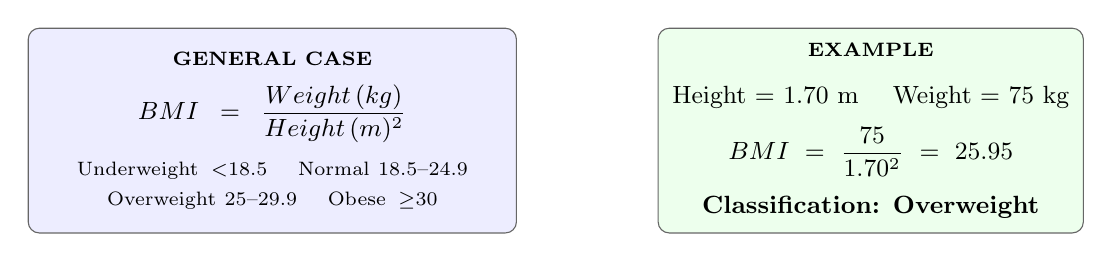
\begin{tikzpicture}[>=Latex]
\node[draw=black!60,rounded corners,fill=blue!7,minimum width=6.2cm,minimum height=2.6cm,align=center,font=\small,text width=5.95cm,inner sep=2pt] (gc_eq) at (0,0) {\textbf{\scriptsize GENERAL CASE}\\[6pt]$BMI = \dfrac{Weight\,(kg)}{Height\,(m)^2}$\\[6pt]\scriptsize Underweight \,$<$18.5 \quad Normal 18.5--24.9\\Overweight 25--29.9 \quad Obese \,$\geq$30};
\node[draw=black!60,rounded corners,fill=green!7,minimum width=5.4cm,minimum height=2.6cm,align=center,font=\small,text width=5.15cm,inner sep=2pt] (ex_body) at (7.6,0) {\textbf{\scriptsize EXAMPLE}\\[6pt]Height = 1.70 m \quad Weight = 75 kg\\[6pt]$BMI = \dfrac{75}{1.70^2} = 25.95$\\[6pt]\textbf{Classification: Overweight}};
\end{tikzpicture}
\end{adjustbox}
\end{center}
\end{frame}

\begin{frame}{Module 1: Basic Health Profile}
\textcolor{black!55}{\scriptsize Schematic 2 -- Input / Output relations}\\[2pt]
\begin{center}
\begin{adjustbox}{max width=0.96\linewidth,max height=0.66\textheight}
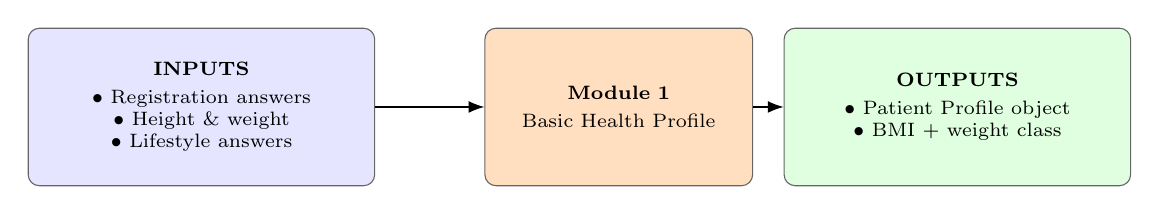
\begin{tikzpicture}[>=Latex]
\node[draw=black!60,rounded corners,fill=blue!10,minimum width=4.4cm,minimum height=2.0cm,align=center,font=\scriptsize,text width=4.15cm,inner sep=2pt] (io_in) at (0,0) {\textbf{\scriptsize INPUTS}\\[2pt]$\bullet$ Registration answers\\$\bullet$ Height \& weight\\$\bullet$ Lifestyle answers};
\node[draw=black!60,rounded corners,fill=orange!25,minimum width=3.4cm,minimum height=2.0cm,align=center,font=\scriptsize,text width=3.15cm,inner sep=2pt] (io_p) at (5.3,0) {\textbf{Module 1}\\[2pt]Basic Health Profile};
\node[draw=black!60,rounded corners,fill=green!12,minimum width=4.4cm,minimum height=2.0cm,align=center,font=\scriptsize,text width=4.15cm,inner sep=2pt] (io_out) at (9.6,0) {\textbf{\scriptsize OUTPUTS}\\[2pt]$\bullet$ Patient Profile object\\$\bullet$ BMI + weight class};
\draw[-{Latex[length=2mm]}] (io_in.east)--(io_p.west);
\draw[-{Latex[length=2mm]}] (io_p.east)--(io_out.west);
\end{tikzpicture}
\end{adjustbox}
\end{center}
\end{frame}

\begin{frame}{Module 2: Blood Report Intake}
\textcolor{black!55}{\scriptsize Cluster 1 -- \textcolor{blue}{\textbf{Intake \& Profiling}} (M1--M3)}\\[2pt]
\begin{columns}[T,onlytextwidth]
\begin{column}{0.5\textwidth}
\begin{tcolorbox}[colback=blue!7,colframe=blue!55!black,title=\textbf{Motivation},boxrule=0.6pt,arc=1mm,left=5pt,right=5pt,top=3pt,bottom=3pt,fonttitle=\small]
\footnotesize Free-text lab reports cannot be reasoned over; the platform needs structured, comparable data.
\end{tcolorbox}
\vspace{5pt}
\begin{tcolorbox}[colback=teal!7,colframe=teal!55!black,title=\textbf{Method},boxrule=0.6pt,arc=1mm,left=5pt,right=5pt,top=3pt,bottom=3pt,fonttitle=\small]
\footnotesize Identify report metadata, then extract each result into a fixed record schema (test, result, unit, reference range, flag, date, source).
\end{tcolorbox}
\end{column}
\begin{column}{0.5\textwidth}
\begin{tcolorbox}[colback=green!8,colframe=green!45!black,title=\textbf{Result},boxrule=0.6pt,arc=1mm,left=5pt,right=5pt,top=3pt,bottom=3pt,fonttitle=\small]
\footnotesize A structured Laboratory Result record for every test on the report.
\end{tcolorbox}
\vspace{5pt}
\begin{tcolorbox}[colback=orange!10,colframe=orange!65!black,title=\textbf{Conclusion},boxrule=0.6pt,arc=1mm,left=5pt,right=5pt,top=3pt,bottom=3pt,fonttitle=\small]
\footnotesize Standardised extraction is the single entry point every later engine ultimately depends on.
\end{tcolorbox}
\end{column}
\end{columns}
\end{frame}

\begin{frame}{Module 2: Blood Report Intake}
\textcolor{black!55}{\scriptsize Schematic 1 -- Two-step intake pipeline}\\[2pt]
\begin{center}
\begin{adjustbox}{max width=0.96\linewidth,max height=0.66\textheight}
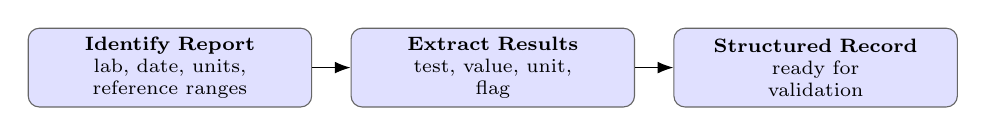
\begin{tikzpicture}[>=Latex]
\node[draw=black!60,rounded corners,fill=blue!12,minimum width=3.6cm,minimum height=1.0cm,align=center,font=\scriptsize,text width=3.35cm,inner sep=2pt] (h0) at (0,0) {\textbf{Identify Report}\\lab, date, units,\\reference ranges};
\node[draw=black!60,rounded corners,fill=blue!12,minimum width=3.6cm,minimum height=1.0cm,align=center,font=\scriptsize,text width=3.35cm,inner sep=2pt] (h1) at (4.1,0) {\textbf{Extract Results}\\test, value, unit,\\flag};
\node[draw=black!60,rounded corners,fill=blue!12,minimum width=3.6cm,minimum height=1.0cm,align=center,font=\scriptsize,text width=3.35cm,inner sep=2pt] (h2) at (8.2,0) {\textbf{Structured Record}\\ready for\\validation};
\draw[-{Latex[length=2mm]}] (h0.east)--(h1.west);
\draw[-{Latex[length=2mm]}] (h1.east)--(h2.west);
\end{tikzpicture}
\end{adjustbox}
\end{center}
\end{frame}

\begin{frame}{Module 2: Blood Report Intake}
\textcolor{black!55}{\scriptsize Schematic 2 -- Input / Output relations}\\[2pt]
\begin{center}
\begin{adjustbox}{max width=0.96\linewidth,max height=0.66\textheight}
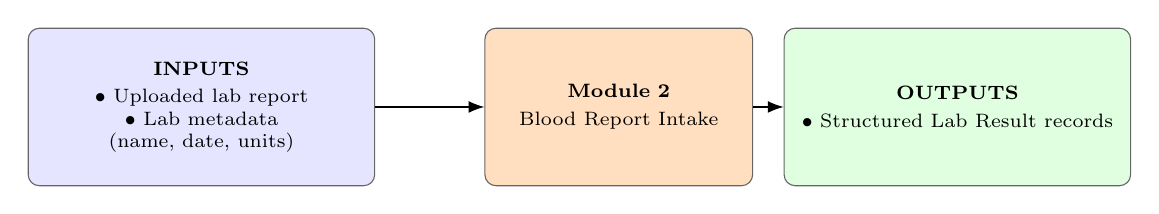
\begin{tikzpicture}[>=Latex]
\node[draw=black!60,rounded corners,fill=blue!10,minimum width=4.4cm,minimum height=2.0cm,align=center,font=\scriptsize,text width=4.15cm,inner sep=2pt] (io_in) at (0,0) {\textbf{\scriptsize INPUTS}\\[2pt]$\bullet$ Uploaded lab report\\$\bullet$ Lab metadata (name, date, units)};
\node[draw=black!60,rounded corners,fill=orange!25,minimum width=3.4cm,minimum height=2.0cm,align=center,font=\scriptsize,text width=3.15cm,inner sep=2pt] (io_p) at (5.3,0) {\textbf{Module 2}\\[2pt]Blood Report Intake};
\node[draw=black!60,rounded corners,fill=green!12,minimum width=4.4cm,minimum height=2.0cm,align=center,font=\scriptsize,text width=4.15cm,inner sep=2pt] (io_out) at (9.6,0) {\textbf{\scriptsize OUTPUTS}\\[2pt]$\bullet$ Structured Lab Result records};
\draw[-{Latex[length=2mm]}] (io_in.east)--(io_p.west);
\draw[-{Latex[length=2mm]}] (io_p.east)--(io_out.west);
\end{tikzpicture}
\end{adjustbox}
\end{center}
\end{frame}

\begin{frame}{Module 3: Data Validation}
\textcolor{black!55}{\scriptsize Cluster 1 -- \textcolor{blue}{\textbf{Intake \& Profiling}} (M1--M3)}\\[2pt]
\begin{columns}[T,onlytextwidth]
\begin{column}{0.5\textwidth}
\begin{tcolorbox}[colback=blue!7,colframe=blue!55!black,title=\textbf{Motivation},boxrule=0.6pt,arc=1mm,left=5pt,right=5pt,top=3pt,bottom=3pt,fonttitle=\small]
\footnotesize An extraction error silently becoming health advice is the platform's single biggest safety risk.
\end{tcolorbox}
\vspace{5pt}
\begin{tcolorbox}[colback=teal!7,colframe=teal!55!black,title=\textbf{Method},boxrule=0.6pt,arc=1mm,left=5pt,right=5pt,top=3pt,bottom=3pt,fonttitle=\small]
\footnotesize Run plausibility checks on every field before interpretation begins; route low-confidence results to explicit user confirmation.
\end{tcolorbox}
\end{column}
\begin{column}{0.5\textwidth}
\begin{tcolorbox}[colback=green!8,colframe=green!45!black,title=\textbf{Result},boxrule=0.6pt,arc=1mm,left=5pt,right=5pt,top=3pt,bottom=3pt,fonttitle=\small]
\footnotesize Either a validated record proceeds automatically, or the user confirms an uncertain reading first.
\end{tcolorbox}
\vspace{5pt}
\begin{tcolorbox}[colback=orange!10,colframe=orange!65!black,title=\textbf{Conclusion},boxrule=0.6pt,arc=1mm,left=5pt,right=5pt,top=3pt,bottom=3pt,fonttitle=\small]
\footnotesize Validation is a gate, not a formality -- nothing reaches interpretation unconfirmed.
\end{tcolorbox}
\end{column}
\end{columns}
\end{frame}

\begin{frame}{Module 3: Data Validation}
\textcolor{black!55}{\scriptsize Schematic 1 -- Six checks feed one confidence decision}\\[2pt]
\begin{center}
\begin{adjustbox}{max width=0.96\linewidth,max height=0.66\textheight}
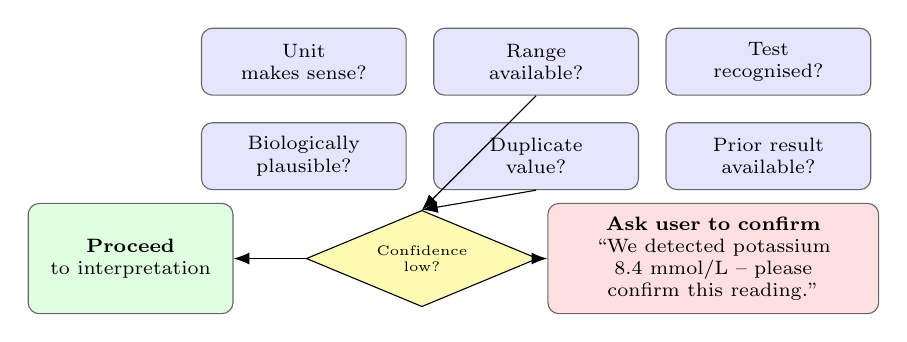
\begin{tikzpicture}[>=Latex]
\node[draw=black!60,rounded corners,fill=blue!10,minimum width=2.6cm,minimum height=0.85cm,align=center,font=\scriptsize,text width=2.35cm,inner sep=2pt] (g0) at (0.0,0.0) {Unit\\makes sense?};
\node[draw=black!60,rounded corners,fill=blue!10,minimum width=2.6cm,minimum height=0.85cm,align=center,font=\scriptsize,text width=2.35cm,inner sep=2pt] (g1) at (2.95,0.0) {Range\\available?};
\node[draw=black!60,rounded corners,fill=blue!10,minimum width=2.6cm,minimum height=0.85cm,align=center,font=\scriptsize,text width=2.35cm,inner sep=2pt] (g2) at (5.9,0.0) {Test\\recognised?};
\node[draw=black!60,rounded corners,fill=blue!10,minimum width=2.6cm,minimum height=0.85cm,align=center,font=\scriptsize,text width=2.35cm,inner sep=2pt] (g3) at (0.0,-1.2) {Biologically\\plausible?};
\node[draw=black!60,rounded corners,fill=blue!10,minimum width=2.6cm,minimum height=0.85cm,align=center,font=\scriptsize,text width=2.35cm,inner sep=2pt] (g4) at (2.95,-1.2) {Duplicate\\value?};
\node[draw=black!60,rounded corners,fill=blue!10,minimum width=2.6cm,minimum height=0.85cm,align=center,font=\scriptsize,text width=2.35cm,inner sep=2pt] (g5) at (5.9,-1.2) {Prior result\\available?};
\node[draw,diamond,aspect=2.4,fill=yellow!30,align=center,font=\tiny,text width=1.9cm,inner sep=1pt] (dv_d) at (1.5,-2.5) {Confidence\\low?};
\draw[-{Latex[length=2mm]}] (g1.south)--(dv_d.north);
\draw[-{Latex[length=2mm]}] (g4.south)--(dv_d.north);
\node[draw=black!60,rounded corners,fill=red!12,minimum width=4.2cm,minimum height=1.4cm,align=center,font=\scriptsize,text width=3.95cm,inner sep=2pt] (dv_yes) at (5.2,-2.5) {\textbf{Ask user to confirm}\\``We detected potassium\\8.4 mmol/L -- please\\confirm this reading.''};
\node[draw=black!60,rounded corners,fill=green!12,minimum width=2.6cm,minimum height=1.4cm,align=center,font=\scriptsize,text width=2.35cm,inner sep=2pt] (dv_no) at (-2.2,-2.5) {\textbf{Proceed}\\to interpretation};
\draw[-{Latex[length=2mm]}] (dv_d.east)--(dv_yes.west);
\draw[-{Latex[length=2mm]}] (dv_d.west)--(dv_no.east);
\end{tikzpicture}
\end{adjustbox}
\end{center}
\end{frame}

\begin{frame}{Module 3: Data Validation}
\textcolor{black!55}{\scriptsize Schematic 2 -- Input / Output relations}\\[2pt]
\begin{center}
\begin{adjustbox}{max width=0.96\linewidth,max height=0.66\textheight}
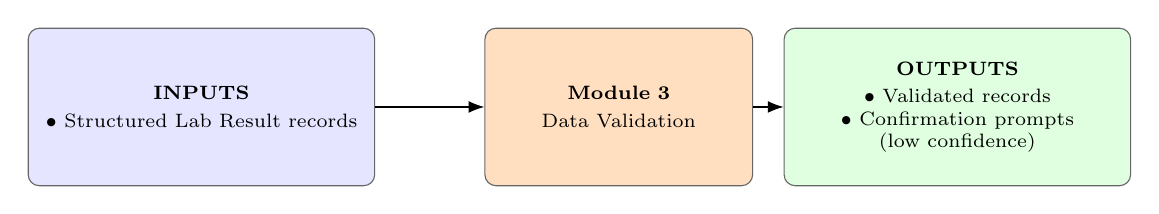
\begin{tikzpicture}[>=Latex]
\node[draw=black!60,rounded corners,fill=blue!10,minimum width=4.4cm,minimum height=2.0cm,align=center,font=\scriptsize,text width=4.15cm,inner sep=2pt] (io_in) at (0,0) {\textbf{\scriptsize INPUTS}\\[2pt]$\bullet$ Structured Lab Result records};
\node[draw=black!60,rounded corners,fill=orange!25,minimum width=3.4cm,minimum height=2.0cm,align=center,font=\scriptsize,text width=3.15cm,inner sep=2pt] (io_p) at (5.3,0) {\textbf{Module 3}\\[2pt]Data Validation};
\node[draw=black!60,rounded corners,fill=green!12,minimum width=4.4cm,minimum height=2.0cm,align=center,font=\scriptsize,text width=4.15cm,inner sep=2pt] (io_out) at (9.6,0) {\textbf{\scriptsize OUTPUTS}\\[2pt]$\bullet$ Validated records\\$\bullet$ Confirmation prompts (low confidence)};
\draw[-{Latex[length=2mm]}] (io_in.east)--(io_p.west);
\draw[-{Latex[length=2mm]}] (io_p.east)--(io_out.west);
\end{tikzpicture}
\end{adjustbox}
\end{center}
\end{frame}

\section{Cluster 2 -- Interpretation (M4--M7)}

\begin{frame}{Module 4: Reference Range Architecture}
\textcolor{black!55}{\scriptsize Cluster 2 -- \textcolor{teal}{\textbf{Interpretation}} (M4--M7)}\\[2pt]
\begin{columns}[T,onlytextwidth]
\begin{column}{0.5\textwidth}
\begin{tcolorbox}[colback=blue!7,colframe=blue!55!black,title=\textbf{Motivation},boxrule=0.6pt,arc=1mm,left=5pt,right=5pt,top=3pt,bottom=3pt,fonttitle=\small]
\footnotesize A single universal reference range cannot serve every lab, guideline and platform rule at once.
\end{tcolorbox}
\vspace{5pt}
\begin{tcolorbox}[colback=teal!7,colframe=teal!55!black,title=\textbf{Method},boxrule=0.6pt,arc=1mm,left=5pt,right=5pt,top=3pt,bottom=3pt,fonttitle=\small]
\footnotesize Layer each marker: the lab's own interval preserved exactly, a recognised clinical threshold, and a platform relative-elevation rule.
\end{tcolorbox}
\end{column}
\begin{column}{0.5\textwidth}
\begin{tcolorbox}[colback=green!8,colframe=green!45!black,title=\textbf{Result},boxrule=0.6pt,arc=1mm,left=5pt,right=5pt,top=3pt,bottom=3pt,fonttitle=\small]
\footnotesize A comparable, lab-independent severity signal for every marker (e.g. 2$\times$ULN).
\end{tcolorbox}
\vspace{5pt}
\begin{tcolorbox}[colback=orange!10,colframe=orange!65!black,title=\textbf{Conclusion},boxrule=0.6pt,arc=1mm,left=5pt,right=5pt,top=3pt,bottom=3pt,fonttitle=\small]
\footnotesize Layering -- not overwriting -- keeps original lab data trustworthy while enabling cross-lab comparison.
\end{tcolorbox}
\end{column}
\end{columns}
\end{frame}

\begin{frame}{Module 4: Reference Range Architecture}
\textcolor{black!55}{\scriptsize Schematic 1 -- Three layers, stacked, not merged}\\[2pt]
\begin{center}
\begin{adjustbox}{max width=0.96\linewidth,max height=0.66\textheight}
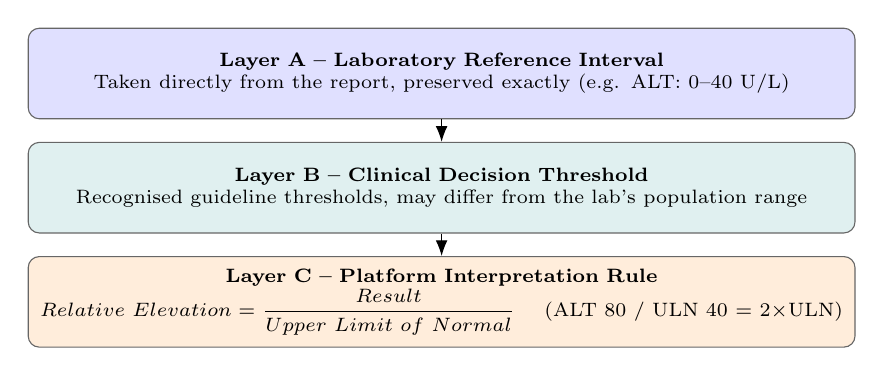
\begin{tikzpicture}[>=Latex]
\node[draw=black!60,rounded corners,fill=blue!12,minimum width=10.5cm,minimum height=1.15cm,align=center,font=\scriptsize,text width=10.25cm,inner sep=2pt] (lv0) at (0,0) {\textbf{Layer A -- Laboratory Reference Interval}\\Taken directly from the report, preserved exactly (e.g. ALT: 0--40 U/L)};
\node[draw=black!60,rounded corners,fill=teal!12,minimum width=10.5cm,minimum height=1.15cm,align=center,font=\scriptsize,text width=10.25cm,inner sep=2pt] (lv1) at (0,-1.45) {\textbf{Layer B -- Clinical Decision Threshold}\\Recognised guideline thresholds, may differ from the lab's population range};
\node[draw=black!60,rounded corners,fill=orange!14,minimum width=10.5cm,minimum height=1.15cm,align=center,font=\scriptsize,text width=10.25cm,inner sep=2pt] (lv2) at (0,-2.9) {\textbf{Layer C -- Platform Interpretation Rule}\\$Relative\ Elevation = \dfrac{Result}{Upper\ Limit\ of\ Normal}$ \quad (ALT 80 / ULN 40 = 2$\times$ULN)};
\draw[-{Latex[length=2mm]}] (lv0.south)--(lv1.north);
\draw[-{Latex[length=2mm]}] (lv1.south)--(lv2.north);
\end{tikzpicture}
\end{adjustbox}
\end{center}
\end{frame}

\begin{frame}{Module 4: Reference Range Architecture}
\textcolor{black!55}{\scriptsize Schematic 2 -- Input / Output relations}\\[2pt]
\begin{center}
\begin{adjustbox}{max width=0.96\linewidth,max height=0.66\textheight}
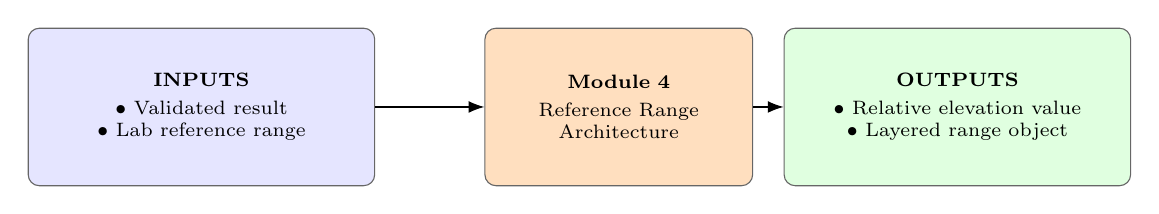
\begin{tikzpicture}[>=Latex]
\node[draw=black!60,rounded corners,fill=blue!10,minimum width=4.4cm,minimum height=2.0cm,align=center,font=\scriptsize,text width=4.15cm,inner sep=2pt] (io_in) at (0,0) {\textbf{\scriptsize INPUTS}\\[2pt]$\bullet$ Validated result\\$\bullet$ Lab reference range};
\node[draw=black!60,rounded corners,fill=orange!25,minimum width=3.4cm,minimum height=2.0cm,align=center,font=\scriptsize,text width=3.15cm,inner sep=2pt] (io_p) at (5.3,0) {\textbf{Module 4}\\[2pt]Reference Range Architecture};
\node[draw=black!60,rounded corners,fill=green!12,minimum width=4.4cm,minimum height=2.0cm,align=center,font=\scriptsize,text width=4.15cm,inner sep=2pt] (io_out) at (9.6,0) {\textbf{\scriptsize OUTPUTS}\\[2pt]$\bullet$ Relative elevation value\\$\bullet$ Layered range object};
\draw[-{Latex[length=2mm]}] (io_in.east)--(io_p.west);
\draw[-{Latex[length=2mm]}] (io_p.east)--(io_out.west);
\end{tikzpicture}
\end{adjustbox}
\end{center}
\end{frame}

\begin{frame}{Module 5: Laboratory Domain Classification}
\textcolor{black!55}{\scriptsize Cluster 2 -- \textcolor{teal}{\textbf{Interpretation}} (M4--M7)}\\[2pt]
\begin{columns}[T,onlytextwidth]
\begin{column}{0.5\textwidth}
\begin{tcolorbox}[colback=blue!7,colframe=blue!55!black,title=\textbf{Motivation},boxrule=0.6pt,arc=1mm,left=5pt,right=5pt,top=3pt,bottom=3pt,fonttitle=\small]
\footnotesize Individual test names mean little without grouping into physiological systems.
\end{tcolorbox}
\vspace{5pt}
\begin{tcolorbox}[colback=teal!7,colframe=teal!55!black,title=\textbf{Method},boxrule=0.6pt,arc=1mm,left=5pt,right=5pt,top=3pt,bottom=3pt,fonttitle=\small]
\footnotesize Map each recognised marker into one or more of eight health domains.
\end{tcolorbox}
\end{column}
\begin{column}{0.5\textwidth}
\begin{tcolorbox}[colback=green!8,colframe=green!45!black,title=\textbf{Result},boxrule=0.6pt,arc=1mm,left=5pt,right=5pt,top=3pt,bottom=3pt,fonttitle=\small]
\footnotesize Every result is tagged with its domain(s), enabling domain-level review and pattern search.
\end{tcolorbox}
\vspace{5pt}
\begin{tcolorbox}[colback=orange!10,colframe=orange!65!black,title=\textbf{Conclusion},boxrule=0.6pt,arc=1mm,left=5pt,right=5pt,top=3pt,bottom=3pt,fonttitle=\small]
\footnotesize Domain tagging is the scaffold that pattern recognition (Module 8) is built on.
\end{tcolorbox}
\end{column}
\end{columns}
\end{frame}

\begin{frame}{Module 5: Laboratory Domain Classification}
\textcolor{black!55}{\scriptsize Schematic 1 -- One test can route to one or more of eight domains}\\[2pt]
\begin{center}
\begin{adjustbox}{max width=0.96\linewidth,max height=0.66\textheight}
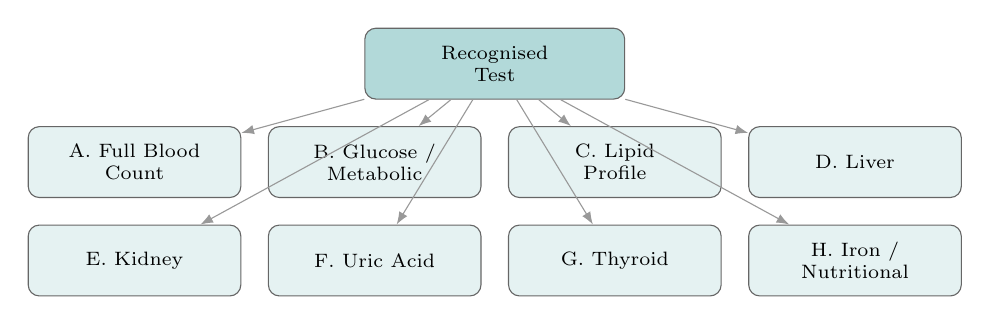
\begin{tikzpicture}[>=Latex]
\node[draw=black!60,rounded corners,fill=teal!10,minimum width=2.7cm,minimum height=0.9cm,align=center,font=\scriptsize,text width=2.45cm,inner sep=2pt] (g0) at (0.0,0.0) {A. Full Blood\\Count};
\node[draw=black!60,rounded corners,fill=teal!10,minimum width=2.7cm,minimum height=0.9cm,align=center,font=\scriptsize,text width=2.45cm,inner sep=2pt] (g1) at (3.0500000000000003,0.0) {B. Glucose /\\Metabolic};
\node[draw=black!60,rounded corners,fill=teal!10,minimum width=2.7cm,minimum height=0.9cm,align=center,font=\scriptsize,text width=2.45cm,inner sep=2pt] (g2) at (6.1000000000000005,0.0) {C. Lipid\\Profile};
\node[draw=black!60,rounded corners,fill=teal!10,minimum width=2.7cm,minimum height=0.9cm,align=center,font=\scriptsize,text width=2.45cm,inner sep=2pt] (g3) at (9.15,0.0) {D. Liver};
\node[draw=black!60,rounded corners,fill=teal!10,minimum width=2.7cm,minimum height=0.9cm,align=center,font=\scriptsize,text width=2.45cm,inner sep=2pt] (g4) at (0.0,-1.25) {E. Kidney};
\node[draw=black!60,rounded corners,fill=teal!10,minimum width=2.7cm,minimum height=0.9cm,align=center,font=\scriptsize,text width=2.45cm,inner sep=2pt] (g5) at (3.0500000000000003,-1.25) {F. Uric Acid};
\node[draw=black!60,rounded corners,fill=teal!10,minimum width=2.7cm,minimum height=0.9cm,align=center,font=\scriptsize,text width=2.45cm,inner sep=2pt] (g6) at (6.1000000000000005,-1.25) {G. Thyroid};
\node[draw=black!60,rounded corners,fill=teal!10,minimum width=2.7cm,minimum height=0.9cm,align=center,font=\scriptsize,text width=2.45cm,inner sep=2pt] (g7) at (9.15,-1.25) {H. Iron /\\Nutritional};
\node[draw=black!60,rounded corners,fill=teal!30,minimum width=3.3000000000000003cm,minimum height=0.9cm,align=center,font=\scriptsize,text width=3.0500000000000003cm,inner sep=2pt] (gc) at (4.575,1.25) {Recognised\\Test};
\draw[-{Latex[length=1.6mm]},black!40] (gc)--(g0);
\draw[-{Latex[length=1.6mm]},black!40] (gc)--(g1);
\draw[-{Latex[length=1.6mm]},black!40] (gc)--(g2);
\draw[-{Latex[length=1.6mm]},black!40] (gc)--(g3);
\draw[-{Latex[length=1.6mm]},black!40] (gc)--(g4);
\draw[-{Latex[length=1.6mm]},black!40] (gc)--(g5);
\draw[-{Latex[length=1.6mm]},black!40] (gc)--(g6);
\draw[-{Latex[length=1.6mm]},black!40] (gc)--(g7);
\end{tikzpicture}
\end{adjustbox}
\end{center}
\end{frame}

\begin{frame}{Module 5: Laboratory Domain Classification}
\textcolor{black!55}{\scriptsize Schematic 2 -- Input / Output relations}\\[2pt]
\begin{center}
\begin{adjustbox}{max width=0.96\linewidth,max height=0.66\textheight}
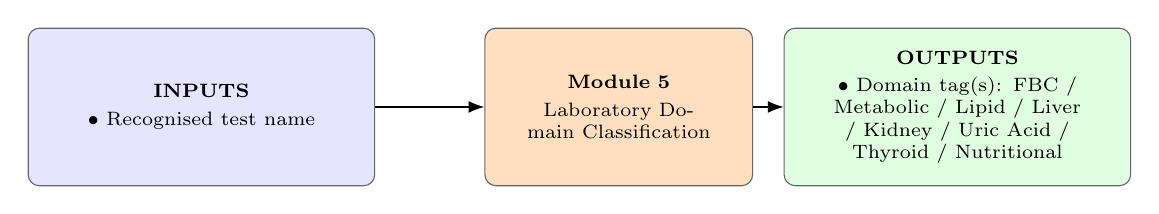
\begin{tikzpicture}[>=Latex]
\node[draw=black!60,rounded corners,fill=blue!10,minimum width=4.4cm,minimum height=2.0cm,align=center,font=\scriptsize,text width=4.15cm,inner sep=2pt] (io_in) at (0,0) {\textbf{\scriptsize INPUTS}\\[2pt]$\bullet$ Recognised test name};
\node[draw=black!60,rounded corners,fill=orange!25,minimum width=3.4cm,minimum height=2.0cm,align=center,font=\scriptsize,text width=3.15cm,inner sep=2pt] (io_p) at (5.3,0) {\textbf{Module 5}\\[2pt]Laboratory Domain Classification};
\node[draw=black!60,rounded corners,fill=green!12,minimum width=4.4cm,minimum height=2.0cm,align=center,font=\scriptsize,text width=4.15cm,inner sep=2pt] (io_out) at (9.6,0) {\textbf{\scriptsize OUTPUTS}\\[2pt]$\bullet$ Domain tag(s): FBC / Metabolic / Lipid / Liver / Kidney / Uric Acid / Thyroid / Nutritional};
\draw[-{Latex[length=2mm]}] (io_in.east)--(io_p.west);
\draw[-{Latex[length=2mm]}] (io_p.east)--(io_out.west);
\end{tikzpicture}
\end{adjustbox}
\end{center}
\end{frame}

\begin{frame}{Module 6: Abnormality Detection}
\textcolor{black!55}{\scriptsize Cluster 2 -- \textcolor{teal}{\textbf{Interpretation}} (M4--M7)}\\[2pt]
\begin{columns}[T,onlytextwidth]
\begin{column}{0.5\textwidth}
\begin{tcolorbox}[colback=blue!7,colframe=blue!55!black,title=\textbf{Motivation},boxrule=0.6pt,arc=1mm,left=5pt,right=5pt,top=3pt,bottom=3pt,fonttitle=\small]
\footnotesize \textquotedblleft Normal / Low / High\textquotedblright\ alone hides how far outside range a value actually is.
\end{tcolorbox}
\vspace{5pt}
\begin{tcolorbox}[colback=teal!7,colframe=teal!55!black,title=\textbf{Method},boxrule=0.6pt,arc=1mm,left=5pt,right=5pt,top=3pt,bottom=3pt,fonttitle=\small]
\footnotesize Assign a basic status (Normal/Low/High), then grade magnitude through a five-step deviation scale.
\end{tcolorbox}
\end{column}
\begin{column}{0.5\textwidth}
\begin{tcolorbox}[colback=green!8,colframe=green!45!black,title=\textbf{Result},boxrule=0.6pt,arc=1mm,left=5pt,right=5pt,top=3pt,bottom=3pt,fonttitle=\small]
\footnotesize Every result carries both a direction and a graded deviation level.
\end{tcolorbox}
\vspace{5pt}
\begin{tcolorbox}[colback=orange!10,colframe=orange!65!black,title=\textbf{Conclusion},boxrule=0.6pt,arc=1mm,left=5pt,right=5pt,top=3pt,bottom=3pt,fonttitle=\small]
\footnotesize Not all \textquotedblleft outside range\textquotedblright\ values are equally important -- magnitude must be visible before severity is assigned.
\end{tcolorbox}
\end{column}
\end{columns}
\end{frame}

\begin{frame}{Module 6: Abnormality Detection}
\textcolor{black!55}{\scriptsize Schematic 1 -- Five-step deviation ladder (green $\to$ red)}\\[2pt]
\begin{center}
\begin{adjustbox}{max width=0.96\linewidth,max height=0.66\textheight}
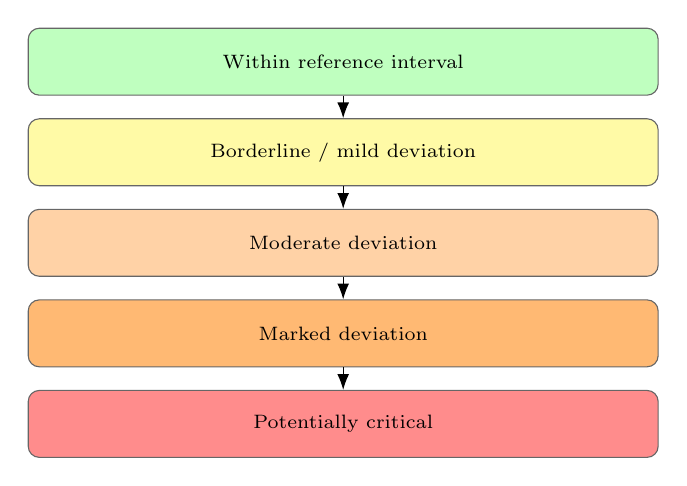
\begin{tikzpicture}[>=Latex]
\node[draw=black!60,rounded corners,fill=green!25,minimum width=8.0cm,minimum height=0.85cm,align=center,font=\scriptsize,text width=7.75cm,inner sep=2pt] (lv0) at (0,0) {Within reference interval};
\node[draw=black!60,rounded corners,fill=yellow!35,minimum width=8.0cm,minimum height=0.85cm,align=center,font=\scriptsize,text width=7.75cm,inner sep=2pt] (lv1) at (0,-1.15) {Borderline / mild deviation};
\node[draw=black!60,rounded corners,fill=orange!35,minimum width=8.0cm,minimum height=0.85cm,align=center,font=\scriptsize,text width=7.75cm,inner sep=2pt] (lv2) at (0,-2.3) {Moderate deviation};
\node[draw=black!60,rounded corners,fill=orange!55,minimum width=8.0cm,minimum height=0.85cm,align=center,font=\scriptsize,text width=7.75cm,inner sep=2pt] (lv3) at (0,-3.4499999999999997) {Marked deviation};
\node[draw=black!60,rounded corners,fill=red!45,minimum width=8.0cm,minimum height=0.85cm,align=center,font=\scriptsize,text width=7.75cm,inner sep=2pt] (lv4) at (0,-4.6) {Potentially critical};
\draw[-{Latex[length=2mm]}] (lv0.south)--(lv1.north);
\draw[-{Latex[length=2mm]}] (lv1.south)--(lv2.north);
\draw[-{Latex[length=2mm]}] (lv2.south)--(lv3.north);
\draw[-{Latex[length=2mm]}] (lv3.south)--(lv4.north);
\end{tikzpicture}
\end{adjustbox}
\end{center}
\end{frame}

\begin{frame}{Module 6: Abnormality Detection}
\textcolor{black!55}{\scriptsize Schematic 2 -- Input / Output relations}\\[2pt]
\begin{center}
\begin{adjustbox}{max width=0.96\linewidth,max height=0.66\textheight}
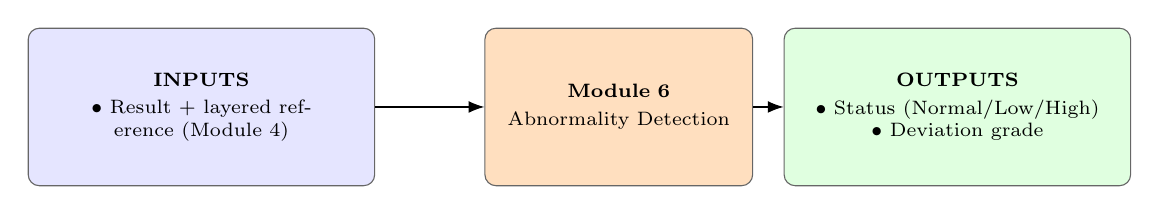
\begin{tikzpicture}[>=Latex]
\node[draw=black!60,rounded corners,fill=blue!10,minimum width=4.4cm,minimum height=2.0cm,align=center,font=\scriptsize,text width=4.15cm,inner sep=2pt] (io_in) at (0,0) {\textbf{\scriptsize INPUTS}\\[2pt]$\bullet$ Result + layered reference (Module 4)};
\node[draw=black!60,rounded corners,fill=orange!25,minimum width=3.4cm,minimum height=2.0cm,align=center,font=\scriptsize,text width=3.15cm,inner sep=2pt] (io_p) at (5.3,0) {\textbf{Module 6}\\[2pt]Abnormality Detection};
\node[draw=black!60,rounded corners,fill=green!12,minimum width=4.4cm,minimum height=2.0cm,align=center,font=\scriptsize,text width=4.15cm,inner sep=2pt] (io_out) at (9.6,0) {\textbf{\scriptsize OUTPUTS}\\[2pt]$\bullet$ Status (Normal/Low/High)\\$\bullet$ Deviation grade};
\draw[-{Latex[length=2mm]}] (io_in.east)--(io_p.west);
\draw[-{Latex[length=2mm]}] (io_p.east)--(io_out.west);
\end{tikzpicture}
\end{adjustbox}
\end{center}
\end{frame}

\begin{frame}{Module 7: Severity Framework}
\textcolor{black!55}{\scriptsize Cluster 2 -- \textcolor{teal}{\textbf{Interpretation}} (M4--M7)}\\[2pt]
\begin{columns}[T,onlytextwidth]
\begin{column}{0.5\textwidth}
\begin{tcolorbox}[colback=blue!7,colframe=blue!55!black,title=\textbf{Motivation},boxrule=0.6pt,arc=1mm,left=5pt,right=5pt,top=3pt,bottom=3pt,fonttitle=\small]
\footnotesize A flat abnormal/normal split cannot route findings to the right next step.
\end{tcolorbox}
\vspace{5pt}
\begin{tcolorbox}[colback=teal!7,colframe=teal!55!black,title=\textbf{Method},boxrule=0.6pt,arc=1mm,left=5pt,right=5pt,top=3pt,bottom=3pt,fonttitle=\small]
\footnotesize Classify every finding into one of six action levels, from optimisation opportunity to potential critical finding.
\end{tcolorbox}
\end{column}
\begin{column}{0.5\textwidth}
\begin{tcolorbox}[colback=green!8,colframe=green!45!black,title=\textbf{Result},boxrule=0.6pt,arc=1mm,left=5pt,right=5pt,top=3pt,bottom=3pt,fonttitle=\small]
\footnotesize A consistent severity label attached to every finding.
\end{tcolorbox}
\vspace{5pt}
\begin{tcolorbox}[colback=orange!10,colframe=orange!65!black,title=\textbf{Conclusion},boxrule=0.6pt,arc=1mm,left=5pt,right=5pt,top=3pt,bottom=3pt,fonttitle=\small]
\footnotesize Severity is the shared vocabulary every later engine (questions, safety, priority) reads from.
\end{tcolorbox}
\end{column}
\end{columns}
\end{frame}

\begin{frame}{Module 7: Severity Framework}
\textcolor{black!55}{\scriptsize Schematic 1 -- Six action levels, escalating risk}\\[2pt]
\begin{center}
\begin{adjustbox}{max width=0.96\linewidth,max height=0.66\textheight}
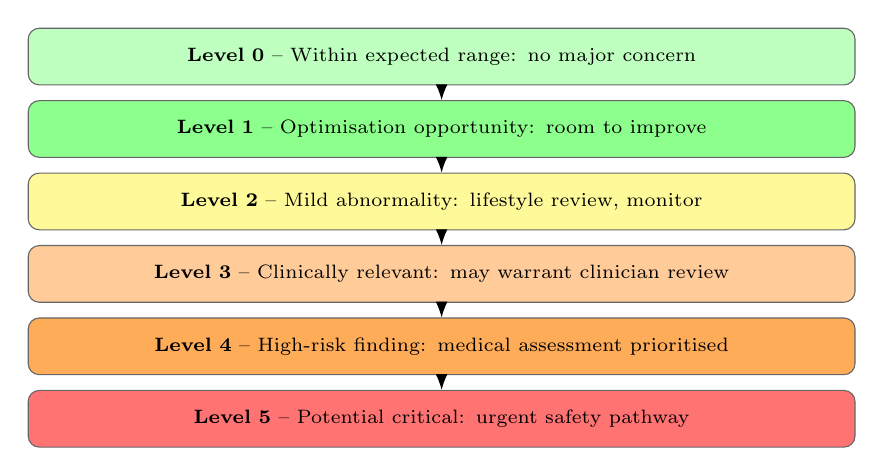
\begin{tikzpicture}[>=Latex]
\node[draw=black!60,rounded corners,fill=green!25,minimum width=10.5cm,minimum height=0.72cm,align=center,font=\scriptsize,text width=10.25cm,inner sep=2pt] (lv0) at (0,0) {\textbf{Level 0} -- Within expected range: no major concern};
\node[draw=black!60,rounded corners,fill=green!45,minimum width=10.5cm,minimum height=0.72cm,align=center,font=\scriptsize,text width=10.25cm,inner sep=2pt] (lv1) at (0,-0.9199999999999999) {\textbf{Level 1} -- Optimisation opportunity: room to improve};
\node[draw=black!60,rounded corners,fill=yellow!40,minimum width=10.5cm,minimum height=0.72cm,align=center,font=\scriptsize,text width=10.25cm,inner sep=2pt] (lv2) at (0,-1.8399999999999999) {\textbf{Level 2} -- Mild abnormality: lifestyle review, monitor};
\node[draw=black!60,rounded corners,fill=orange!40,minimum width=10.5cm,minimum height=0.72cm,align=center,font=\scriptsize,text width=10.25cm,inner sep=2pt] (lv3) at (0,-2.76) {\textbf{Level 3} -- Clinically relevant: may warrant clinician review};
\node[draw=black!60,rounded corners,fill=orange!65,minimum width=10.5cm,minimum height=0.72cm,align=center,font=\scriptsize,text width=10.25cm,inner sep=2pt] (lv4) at (0,-3.6799999999999997) {\textbf{Level 4} -- High-risk finding: medical assessment prioritised};
\node[draw=black!60,rounded corners,fill=red!55,minimum width=10.5cm,minimum height=0.72cm,align=center,font=\scriptsize,text width=10.25cm,inner sep=2pt] (lv5) at (0,-4.6) {\textbf{Level 5} -- Potential critical: urgent safety pathway};
\draw[-{Latex[length=2mm]}] (lv0.south)--(lv1.north);
\draw[-{Latex[length=2mm]}] (lv1.south)--(lv2.north);
\draw[-{Latex[length=2mm]}] (lv2.south)--(lv3.north);
\draw[-{Latex[length=2mm]}] (lv3.south)--(lv4.north);
\draw[-{Latex[length=2mm]}] (lv4.south)--(lv5.north);
\end{tikzpicture}
\end{adjustbox}
\end{center}
\end{frame}

\begin{frame}{Module 7: Severity Framework}
\textcolor{black!55}{\scriptsize Schematic 2 -- Input / Output relations}\\[2pt]
\begin{center}
\begin{adjustbox}{max width=0.96\linewidth,max height=0.66\textheight}
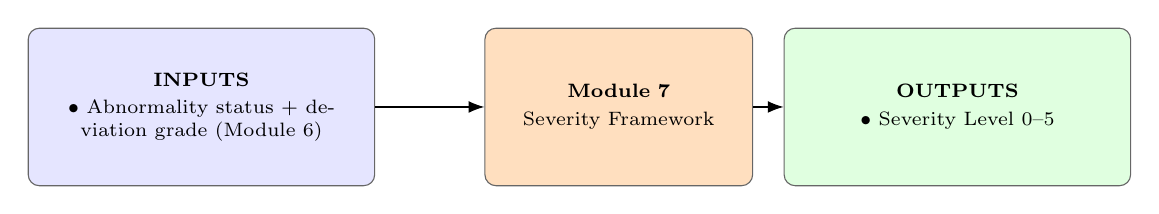
\begin{tikzpicture}[>=Latex]
\node[draw=black!60,rounded corners,fill=blue!10,minimum width=4.4cm,minimum height=2.0cm,align=center,font=\scriptsize,text width=4.15cm,inner sep=2pt] (io_in) at (0,0) {\textbf{\scriptsize INPUTS}\\[2pt]$\bullet$ Abnormality status + deviation grade (Module 6)};
\node[draw=black!60,rounded corners,fill=orange!25,minimum width=3.4cm,minimum height=2.0cm,align=center,font=\scriptsize,text width=3.15cm,inner sep=2pt] (io_p) at (5.3,0) {\textbf{Module 7}\\[2pt]Severity Framework};
\node[draw=black!60,rounded corners,fill=green!12,minimum width=4.4cm,minimum height=2.0cm,align=center,font=\scriptsize,text width=4.15cm,inner sep=2pt] (io_out) at (9.6,0) {\textbf{\scriptsize OUTPUTS}\\[2pt]$\bullet$ Severity Level 0--5};
\draw[-{Latex[length=2mm]}] (io_in.east)--(io_p.west);
\draw[-{Latex[length=2mm]}] (io_p.east)--(io_out.west);
\end{tikzpicture}
\end{adjustbox}
\end{center}
\end{frame}

\section{Cluster 3 -- Pattern \& Trigger (M8--M9)}

\begin{frame}{Module 8: Pattern Recognition Engine}
\textcolor{black!55}{\scriptsize Cluster 3 -- \textcolor{violet}{\textbf{Pattern \& Trigger}} (M8--M9)}\\[2pt]
\begin{columns}[T,onlytextwidth]
\begin{column}{0.5\textwidth}
\begin{tcolorbox}[colback=blue!7,colframe=blue!55!black,title=\textbf{Motivation},boxrule=0.6pt,arc=1mm,left=5pt,right=5pt,top=3pt,bottom=3pt,fonttitle=\small]
\footnotesize Treating each abnormal value independently misses the clinical picture combinations reveal.
\end{tcolorbox}
\vspace{5pt}
\begin{tcolorbox}[colback=teal!7,colframe=teal!55!black,title=\textbf{Method},boxrule=0.6pt,arc=1mm,left=5pt,right=5pt,top=3pt,bottom=3pt,fonttitle=\small]
\footnotesize Search for known marker combinations (metabolic, microcytic, liver) across domains rather than single values.
\end{tcolorbox}
\end{column}
\begin{column}{0.5\textwidth}
\begin{tcolorbox}[colback=green!8,colframe=green!45!black,title=\textbf{Result},boxrule=0.6pt,arc=1mm,left=5pt,right=5pt,top=3pt,bottom=3pt,fonttitle=\small]
\footnotesize Named patterns -- e.g. \textquotedblleft metabolic-risk pattern\textquotedblright\ -- attached to the finding set (never a diagnosis).
\end{tcolorbox}
\vspace{5pt}
\begin{tcolorbox}[colback=orange!10,colframe=orange!65!black,title=\textbf{Conclusion},boxrule=0.6pt,arc=1mm,left=5pt,right=5pt,top=3pt,bottom=3pt,fonttitle=\small]
\footnotesize Patterns turn a list of abnormal numbers into a coherent health narrative.
\end{tcolorbox}
\end{column}
\end{columns}
\end{frame}

\begin{frame}{Module 8: Pattern Recognition Engine}
\textcolor{black!55}{\scriptsize Schematic 1 -- Three worked pattern examples}\\[2pt]
\begin{center}
\begin{adjustbox}{max width=0.96\linewidth,max height=0.66\textheight}
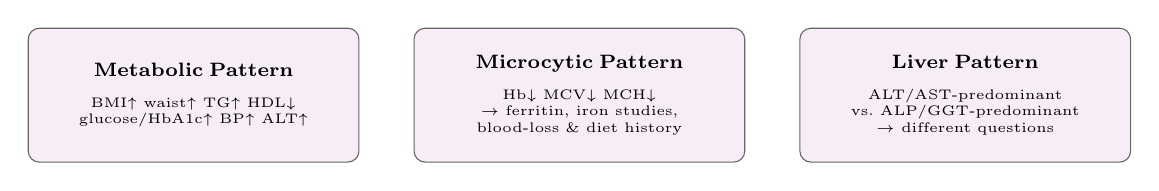
\begin{tikzpicture}[>=Latex]
\node[draw=black!60,rounded corners,fill=violet!7,minimum width=4.2cm,minimum height=1.7cm,align=center,font=\tiny,text width=3.95cm,inner sep=2pt] (p8b1) at (0,0) {\textbf{\scriptsize Metabolic Pattern}\\[5pt]BMI$\uparrow$ waist$\uparrow$ TG$\uparrow$ HDL$\downarrow$\\glucose/HbA1c$\uparrow$ BP$\uparrow$ ALT$\uparrow$};
\node[draw=black!60,rounded corners,fill=violet!7,minimum width=4.2cm,minimum height=1.7cm,align=center,font=\tiny,text width=3.95cm,inner sep=2pt] (p8b2) at (4.9,0) {\textbf{\scriptsize Microcytic Pattern}\\[5pt]Hb$\downarrow$ MCV$\downarrow$ MCH$\downarrow$\\$\to$ ferritin, iron studies,\\blood-loss \& diet history};
\node[draw=black!60,rounded corners,fill=violet!7,minimum width=4.2cm,minimum height=1.7cm,align=center,font=\tiny,text width=3.95cm,inner sep=2pt] (p8b3) at (9.8,0) {\textbf{\scriptsize Liver Pattern}\\[5pt]ALT/AST-predominant\\vs.\ ALP/GGT-predominant\\$\to$ different questions};
\end{tikzpicture}
\end{adjustbox}
\end{center}
\end{frame}

\begin{frame}{Module 8: Pattern Recognition Engine}
\textcolor{black!55}{\scriptsize Schematic 2 -- Input / Output relations}\\[2pt]
\begin{center}
\begin{adjustbox}{max width=0.96\linewidth,max height=0.66\textheight}
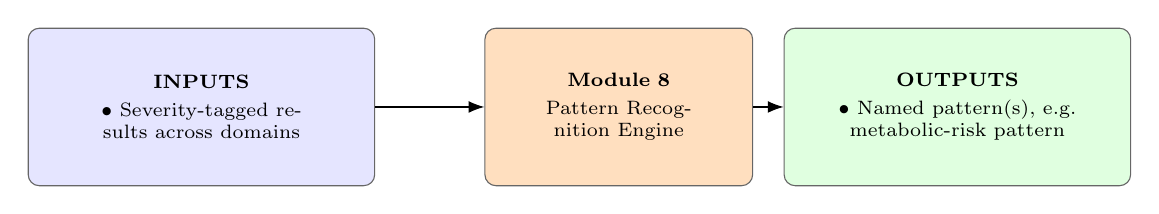
\begin{tikzpicture}[>=Latex]
\node[draw=black!60,rounded corners,fill=blue!10,minimum width=4.4cm,minimum height=2.0cm,align=center,font=\scriptsize,text width=4.15cm,inner sep=2pt] (io_in) at (0,0) {\textbf{\scriptsize INPUTS}\\[2pt]$\bullet$ Severity-tagged results across domains};
\node[draw=black!60,rounded corners,fill=orange!25,minimum width=3.4cm,minimum height=2.0cm,align=center,font=\scriptsize,text width=3.15cm,inner sep=2pt] (io_p) at (5.3,0) {\textbf{Module 8}\\[2pt]Pattern Recognition Engine};
\node[draw=black!60,rounded corners,fill=green!12,minimum width=4.4cm,minimum height=2.0cm,align=center,font=\scriptsize,text width=4.15cm,inner sep=2pt] (io_out) at (9.6,0) {\textbf{\scriptsize OUTPUTS}\\[2pt]$\bullet$ Named pattern(s), e.g. metabolic-risk pattern};
\draw[-{Latex[length=2mm]}] (io_in.east)--(io_p.west);
\draw[-{Latex[length=2mm]}] (io_p.east)--(io_out.west);
\end{tikzpicture}
\end{adjustbox}
\end{center}
\end{frame}

\begin{frame}{Module 9: Master Trigger Matrix}
\textcolor{black!55}{\scriptsize Cluster 3 -- \textcolor{violet}{\textbf{Pattern \& Trigger}} (M8--M9)}\\[2pt]
\begin{columns}[T,onlytextwidth]
\begin{column}{0.5\textwidth}
\begin{tcolorbox}[colback=blue!7,colframe=blue!55!black,title=\textbf{Motivation},boxrule=0.6pt,arc=1mm,left=5pt,right=5pt,top=3pt,bottom=3pt,fonttitle=\small]
\footnotesize Asking every possible question overwhelms the user; asking none misses context.
\end{tcolorbox}
\vspace{5pt}
\begin{tcolorbox}[colback=teal!7,colframe=teal!55!black,title=\textbf{Method},boxrule=0.6pt,arc=1mm,left=5pt,right=5pt,top=3pt,bottom=3pt,fonttitle=\small]
\footnotesize Map each finding/pattern to the specific trigger conditions that activate a targeted question set.
\end{tcolorbox}
\end{column}
\begin{column}{0.5\textwidth}
\begin{tcolorbox}[colback=green!8,colframe=green!45!black,title=\textbf{Result},boxrule=0.6pt,arc=1mm,left=5pt,right=5pt,top=3pt,bottom=3pt,fonttitle=\small]
\footnotesize A minimal, finding-specific question list per patient.
\end{tcolorbox}
\vspace{5pt}
\begin{tcolorbox}[colback=orange!10,colframe=orange!65!black,title=\textbf{Conclusion},boxrule=0.6pt,arc=1mm,left=5pt,right=5pt,top=3pt,bottom=3pt,fonttitle=\small]
\footnotesize The matrix is the switchboard connecting findings to exactly the right follow-up questions.
\end{tcolorbox}
\end{column}
\end{columns}
\end{frame}

\begin{frame}{Module 9: Master Trigger Matrix}
\textcolor{black!55}{\scriptsize Schematic 1 -- Finding $\to$ Pattern $\to$ Trigger $\to$ Questions}\\[2pt]
\begin{center}
\begin{adjustbox}{max width=0.96\linewidth,max height=0.66\textheight}
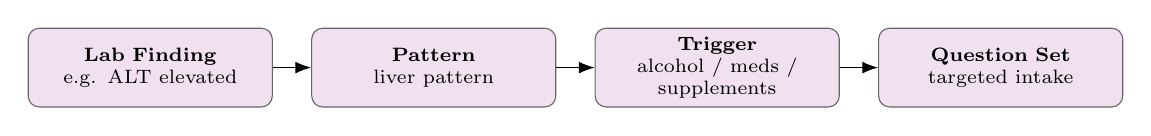
\begin{tikzpicture}[>=Latex]
\node[draw=black!60,rounded corners,fill=violet!12,minimum width=3.1cm,minimum height=1.0cm,align=center,font=\scriptsize,text width=2.85cm,inner sep=2pt] (h0) at (0,0) {\textbf{Lab Finding}\\e.g. ALT elevated};
\node[draw=black!60,rounded corners,fill=violet!12,minimum width=3.1cm,minimum height=1.0cm,align=center,font=\scriptsize,text width=2.85cm,inner sep=2pt] (h1) at (3.6,0) {\textbf{Pattern}\\liver pattern};
\node[draw=black!60,rounded corners,fill=violet!12,minimum width=3.1cm,minimum height=1.0cm,align=center,font=\scriptsize,text width=2.85cm,inner sep=2pt] (h2) at (7.2,0) {\textbf{Trigger}\\alcohol / meds /\\supplements};
\node[draw=black!60,rounded corners,fill=violet!12,minimum width=3.1cm,minimum height=1.0cm,align=center,font=\scriptsize,text width=2.85cm,inner sep=2pt] (h3) at (10.8,0) {\textbf{Question Set}\\targeted intake};
\draw[-{Latex[length=2mm]}] (h0.east)--(h1.west);
\draw[-{Latex[length=2mm]}] (h1.east)--(h2.west);
\draw[-{Latex[length=2mm]}] (h2.east)--(h3.west);
\end{tikzpicture}
\end{adjustbox}
\end{center}
\end{frame}

\begin{frame}{Module 9: Master Trigger Matrix}
\textcolor{black!55}{\scriptsize Schematic 2 -- Input / Output relations}\\[2pt]
\begin{center}
\begin{adjustbox}{max width=0.96\linewidth,max height=0.66\textheight}
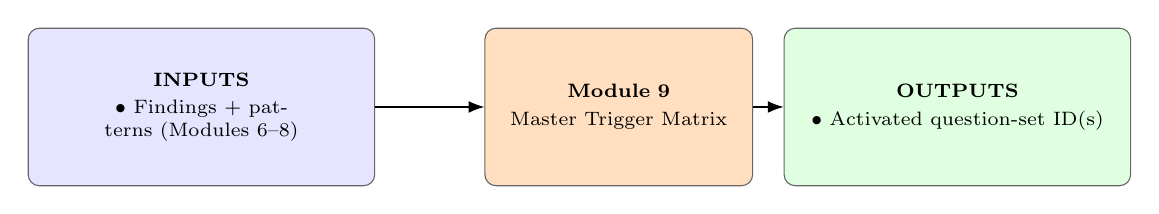
\begin{tikzpicture}[>=Latex]
\node[draw=black!60,rounded corners,fill=blue!10,minimum width=4.4cm,minimum height=2.0cm,align=center,font=\scriptsize,text width=4.15cm,inner sep=2pt] (io_in) at (0,0) {\textbf{\scriptsize INPUTS}\\[2pt]$\bullet$ Findings + patterns (Modules 6--8)};
\node[draw=black!60,rounded corners,fill=orange!25,minimum width=3.4cm,minimum height=2.0cm,align=center,font=\scriptsize,text width=3.15cm,inner sep=2pt] (io_p) at (5.3,0) {\textbf{Module 9}\\[2pt]Master Trigger Matrix};
\node[draw=black!60,rounded corners,fill=green!12,minimum width=4.4cm,minimum height=2.0cm,align=center,font=\scriptsize,text width=4.15cm,inner sep=2pt] (io_out) at (9.6,0) {\textbf{\scriptsize OUTPUTS}\\[2pt]$\bullet$ Activated question-set ID(s)};
\draw[-{Latex[length=2mm]}] (io_in.east)--(io_p.west);
\draw[-{Latex[length=2mm]}] (io_p.east)--(io_out.west);
\end{tikzpicture}
\end{adjustbox}
\end{center}
\end{frame}

\section{Cluster 4 -- Context \& Questions (M10--M11)}

\begin{frame}{Module 10: Targeted Question Engine}
\textcolor{black!55}{\scriptsize Cluster 4 -- \textcolor{orange}{\textbf{Context \& Questions}} (M10--M11)}\\[2pt]
\begin{columns}[T,onlytextwidth]
\begin{column}{0.5\textwidth}
\begin{tcolorbox}[colback=blue!7,colframe=blue!55!black,title=\textbf{Motivation},boxrule=0.6pt,arc=1mm,left=5pt,right=5pt,top=3pt,bottom=3pt,fonttitle=\small]
\footnotesize A full intake questionnaire is unnecessary and burdensome when only specific findings need context.
\end{tcolorbox}
\vspace{5pt}
\begin{tcolorbox}[colback=teal!7,colframe=teal!55!black,title=\textbf{Method},boxrule=0.6pt,arc=1mm,left=5pt,right=5pt,top=3pt,bottom=3pt,fonttitle=\small]
\footnotesize Organise questions into seven categories and activate only the categories a trigger has switched on.
\end{tcolorbox}
\end{column}
\begin{column}{0.5\textwidth}
\begin{tcolorbox}[colback=green!8,colframe=green!45!black,title=\textbf{Result},boxrule=0.6pt,arc=1mm,left=5pt,right=5pt,top=3pt,bottom=3pt,fonttitle=\small]
\footnotesize A short, finding-specific question set the patient actually answers.
\end{tcolorbox}
\vspace{5pt}
\begin{tcolorbox}[colback=orange!10,colframe=orange!65!black,title=\textbf{Conclusion},boxrule=0.6pt,arc=1mm,left=5pt,right=5pt,top=3pt,bottom=3pt,fonttitle=\small]
\footnotesize Precision questioning keeps engagement high without sacrificing clinical context.
\end{tcolorbox}
\end{column}
\end{columns}
\end{frame}

\begin{frame}{Module 10: Targeted Question Engine}
\textcolor{black!55}{\scriptsize Schematic 1 -- Seven question categories, activated selectively}\\[2pt]
\begin{center}
\begin{adjustbox}{max width=0.96\linewidth,max height=0.66\textheight}
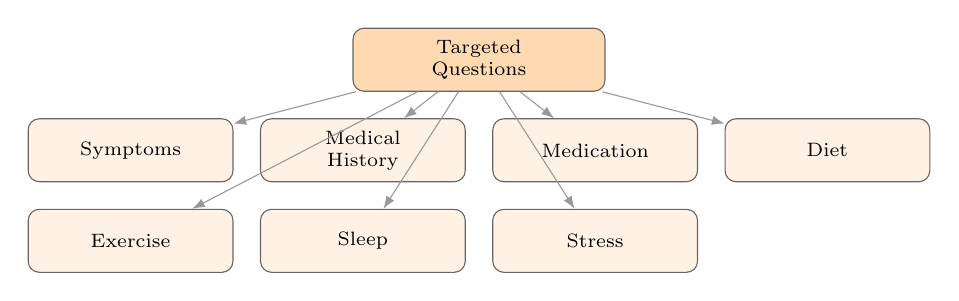
\begin{tikzpicture}[>=Latex]
\node[draw=black!60,rounded corners,fill=orange!10,minimum width=2.6cm,minimum height=0.8cm,align=center,font=\scriptsize,text width=2.35cm,inner sep=2pt] (g0) at (0.0,0.0) {Symptoms};
\node[draw=black!60,rounded corners,fill=orange!10,minimum width=2.6cm,minimum height=0.8cm,align=center,font=\scriptsize,text width=2.35cm,inner sep=2pt] (g1) at (2.95,0.0) {Medical\\History};
\node[draw=black!60,rounded corners,fill=orange!10,minimum width=2.6cm,minimum height=0.8cm,align=center,font=\scriptsize,text width=2.35cm,inner sep=2pt] (g2) at (5.9,0.0) {Medication};
\node[draw=black!60,rounded corners,fill=orange!10,minimum width=2.6cm,minimum height=0.8cm,align=center,font=\scriptsize,text width=2.35cm,inner sep=2pt] (g3) at (8.850000000000001,0.0) {Diet};
\node[draw=black!60,rounded corners,fill=orange!10,minimum width=2.6cm,minimum height=0.8cm,align=center,font=\scriptsize,text width=2.35cm,inner sep=2pt] (g4) at (0.0,-1.15) {Exercise};
\node[draw=black!60,rounded corners,fill=orange!10,minimum width=2.6cm,minimum height=0.8cm,align=center,font=\scriptsize,text width=2.35cm,inner sep=2pt] (g5) at (2.95,-1.15) {Sleep};
\node[draw=black!60,rounded corners,fill=orange!10,minimum width=2.6cm,minimum height=0.8cm,align=center,font=\scriptsize,text width=2.35cm,inner sep=2pt] (g6) at (5.9,-1.15) {Stress};
\node[draw=black!60,rounded corners,fill=orange!30,minimum width=3.2cm,minimum height=0.8cm,align=center,font=\scriptsize,text width=2.95cm,inner sep=2pt] (gc) at (4.425000000000001,1.15) {Targeted\\Questions};
\draw[-{Latex[length=1.6mm]},black!40] (gc)--(g0);
\draw[-{Latex[length=1.6mm]},black!40] (gc)--(g1);
\draw[-{Latex[length=1.6mm]},black!40] (gc)--(g2);
\draw[-{Latex[length=1.6mm]},black!40] (gc)--(g3);
\draw[-{Latex[length=1.6mm]},black!40] (gc)--(g4);
\draw[-{Latex[length=1.6mm]},black!40] (gc)--(g5);
\draw[-{Latex[length=1.6mm]},black!40] (gc)--(g6);
\end{tikzpicture}
\end{adjustbox}
\end{center}
\end{frame}

\begin{frame}{Module 10: Targeted Question Engine}
\textcolor{black!55}{\scriptsize Schematic 2 -- Input / Output relations}\\[2pt]
\begin{center}
\begin{adjustbox}{max width=0.96\linewidth,max height=0.66\textheight}
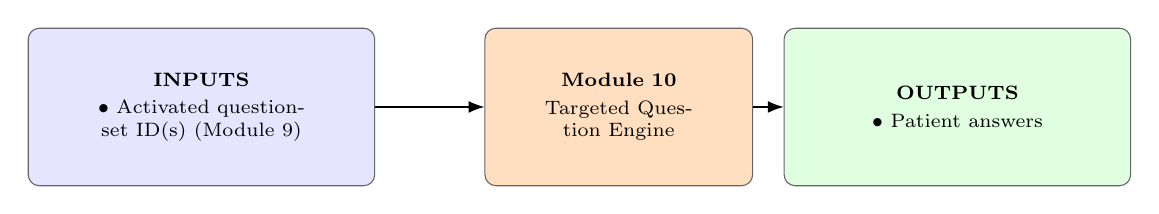
\begin{tikzpicture}[>=Latex]
\node[draw=black!60,rounded corners,fill=blue!10,minimum width=4.4cm,minimum height=2.0cm,align=center,font=\scriptsize,text width=4.15cm,inner sep=2pt] (io_in) at (0,0) {\textbf{\scriptsize INPUTS}\\[2pt]$\bullet$ Activated question-set ID(s) (Module 9)};
\node[draw=black!60,rounded corners,fill=orange!25,minimum width=3.4cm,minimum height=2.0cm,align=center,font=\scriptsize,text width=3.15cm,inner sep=2pt] (io_p) at (5.3,0) {\textbf{Module 10}\\[2pt]Targeted Question Engine};
\node[draw=black!60,rounded corners,fill=green!12,minimum width=4.4cm,minimum height=2.0cm,align=center,font=\scriptsize,text width=4.15cm,inner sep=2pt] (io_out) at (9.6,0) {\textbf{\scriptsize OUTPUTS}\\[2pt]$\bullet$ Patient answers};
\draw[-{Latex[length=2mm]}] (io_in.east)--(io_p.west);
\draw[-{Latex[length=2mm]}] (io_p.east)--(io_out.west);
\end{tikzpicture}
\end{adjustbox}
\end{center}
\end{frame}

\begin{frame}{Module 11: Context Integration Engine}
\textcolor{black!55}{\scriptsize Cluster 4 -- \textcolor{orange}{\textbf{Context \& Questions}} (M10--M11)}\\[2pt]
\begin{columns}[T,onlytextwidth]
\begin{column}{0.5\textwidth}
\begin{tcolorbox}[colback=blue!7,colframe=blue!55!black,title=\textbf{Motivation},boxrule=0.6pt,arc=1mm,left=5pt,right=5pt,top=3pt,bottom=3pt,fonttitle=\small]
\footnotesize A recommendation built from lab data alone ignores the person behind the numbers.
\end{tcolorbox}
\vspace{5pt}
\begin{tcolorbox}[colback=teal!7,colframe=teal!55!black,title=\textbf{Method},boxrule=0.6pt,arc=1mm,left=5pt,right=5pt,top=3pt,bottom=3pt,fonttitle=\small]
\footnotesize Merge lab results with profile, history, medication, symptoms, lifestyle and previous results into one context object.
\end{tcolorbox}
\end{column}
\begin{column}{0.5\textwidth}
\begin{tcolorbox}[colback=green!8,colframe=green!45!black,title=\textbf{Result},boxrule=0.6pt,arc=1mm,left=5pt,right=5pt,top=3pt,bottom=3pt,fonttitle=\small]
\footnotesize A single, unified Health Context used by every downstream engine.
\end{tcolorbox}
\vspace{5pt}
\begin{tcolorbox}[colback=orange!10,colframe=orange!65!black,title=\textbf{Conclusion},boxrule=0.6pt,arc=1mm,left=5pt,right=5pt,top=3pt,bottom=3pt,fonttitle=\small]
\footnotesize Integration is what turns isolated data streams into one coherent case.
\end{tcolorbox}
\end{column}
\end{columns}
\end{frame}

\begin{frame}{Module 11: Context Integration Engine}
\textcolor{black!55}{\scriptsize Schematic 1 -- Seven inputs converge into one context object}\\[2pt]
\begin{center}
\begin{adjustbox}{max width=0.96\linewidth,max height=0.66\textheight}
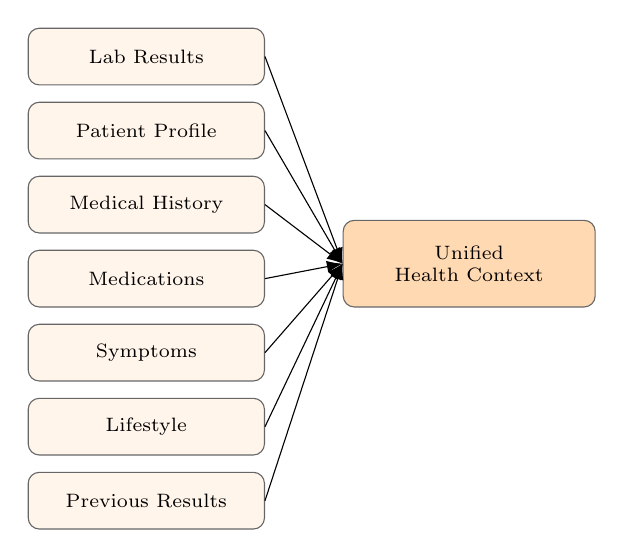
\begin{tikzpicture}[>=Latex]
\node[draw=black!60,rounded corners,fill=orange!8,minimum width=3.0cm,minimum height=0.72cm,align=center,font=\scriptsize,text width=2.75cm,inner sep=2pt] (in0) at (0,0) {Lab Results};
\node[draw=black!60,rounded corners,fill=orange!8,minimum width=3.0cm,minimum height=0.72cm,align=center,font=\scriptsize,text width=2.75cm,inner sep=2pt] (in1) at (0,-0.94) {Patient Profile};
\node[draw=black!60,rounded corners,fill=orange!8,minimum width=3.0cm,minimum height=0.72cm,align=center,font=\scriptsize,text width=2.75cm,inner sep=2pt] (in2) at (0,-1.88) {Medical History};
\node[draw=black!60,rounded corners,fill=orange!8,minimum width=3.0cm,minimum height=0.72cm,align=center,font=\scriptsize,text width=2.75cm,inner sep=2pt] (in3) at (0,-2.82) {Medications};
\node[draw=black!60,rounded corners,fill=orange!8,minimum width=3.0cm,minimum height=0.72cm,align=center,font=\scriptsize,text width=2.75cm,inner sep=2pt] (in4) at (0,-3.76) {Symptoms};
\node[draw=black!60,rounded corners,fill=orange!8,minimum width=3.0cm,minimum height=0.72cm,align=center,font=\scriptsize,text width=2.75cm,inner sep=2pt] (in5) at (0,-4.699999999999999) {Lifestyle};
\node[draw=black!60,rounded corners,fill=orange!8,minimum width=3.0cm,minimum height=0.72cm,align=center,font=\scriptsize,text width=2.75cm,inner sep=2pt] (in6) at (0,-5.639999999999999) {Previous Results};
\node[draw=black!60,rounded corners,fill=orange!30,minimum width=3.2cm,minimum height=1.1cm,align=center,font=\scriptsize,text width=2.95cm,inner sep=2pt] (cc2) at (4.1,-2.63) {Unified\\Health Context};
\draw[-{Latex[length=2mm]}] (in0.east)--(cc2.west);
\draw[-{Latex[length=2mm]}] (in1.east)--(cc2.west);
\draw[-{Latex[length=2mm]}] (in2.east)--(cc2.west);
\draw[-{Latex[length=2mm]}] (in3.east)--(cc2.west);
\draw[-{Latex[length=2mm]}] (in4.east)--(cc2.west);
\draw[-{Latex[length=2mm]}] (in5.east)--(cc2.west);
\draw[-{Latex[length=2mm]}] (in6.east)--(cc2.west);
\end{tikzpicture}
\end{adjustbox}
\end{center}
\end{frame}

\begin{frame}{Module 11: Context Integration Engine}
\textcolor{black!55}{\scriptsize Schematic 2 -- Input / Output relations}\\[2pt]
\begin{center}
\begin{adjustbox}{max width=0.96\linewidth,max height=0.66\textheight}
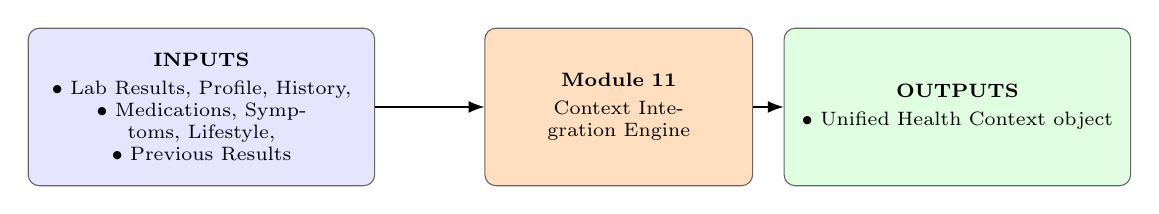
\begin{tikzpicture}[>=Latex]
\node[draw=black!60,rounded corners,fill=blue!10,minimum width=4.4cm,minimum height=2.0cm,align=center,font=\scriptsize,text width=4.15cm,inner sep=2pt] (io_in) at (0,0) {\textbf{\scriptsize INPUTS}\\[2pt]$\bullet$ Lab Results, Profile, History,\\$\bullet$ Medications, Symptoms, Lifestyle,\\$\bullet$ Previous Results};
\node[draw=black!60,rounded corners,fill=orange!25,minimum width=3.4cm,minimum height=2.0cm,align=center,font=\scriptsize,text width=3.15cm,inner sep=2pt] (io_p) at (5.3,0) {\textbf{Module 11}\\[2pt]Context Integration Engine};
\node[draw=black!60,rounded corners,fill=green!12,minimum width=4.4cm,minimum height=2.0cm,align=center,font=\scriptsize,text width=4.15cm,inner sep=2pt] (io_out) at (9.6,0) {\textbf{\scriptsize OUTPUTS}\\[2pt]$\bullet$ Unified Health Context object};
\draw[-{Latex[length=2mm]}] (io_in.east)--(io_p.west);
\draw[-{Latex[length=2mm]}] (io_p.east)--(io_out.west);
\end{tikzpicture}
\end{adjustbox}
\end{center}
\end{frame}

\section{Cluster 5 -- Safety \& Priority (M12--M14)}

\begin{frame}{Module 12: Safety and Referral Engine}
\textcolor{black!55}{\scriptsize Cluster 5 -- \textcolor{red}{\textbf{Safety \& Priority}} (M12--M14)}\\[2pt]
\begin{columns}[T,onlytextwidth]
\begin{column}{0.5\textwidth}
\begin{tcolorbox}[colback=blue!7,colframe=blue!55!black,title=\textbf{Motivation},boxrule=0.6pt,arc=1mm,left=5pt,right=5pt,top=3pt,bottom=3pt,fonttitle=\small]
\footnotesize Wellness advice must never mask a finding that needs medical attention.
\end{tcolorbox}
\vspace{5pt}
\begin{tcolorbox}[colback=teal!7,colframe=teal!55!black,title=\textbf{Method},boxrule=0.6pt,arc=1mm,left=5pt,right=5pt,top=3pt,bottom=3pt,fonttitle=\small]
\footnotesize Ask \textquotedblleft is this appropriate for routine wellness guidance?\textquotedblright\ before any recommendation is generated.
\end{tcolorbox}
\end{column}
\begin{column}{0.5\textwidth}
\begin{tcolorbox}[colback=green!8,colframe=green!45!black,title=\textbf{Result},boxrule=0.6pt,arc=1mm,left=5pt,right=5pt,top=3pt,bottom=3pt,fonttitle=\small]
\footnotesize Every case is routed to Routine Wellness, Medical Review, Prompt Assessment, or Urgent Assessment.
\end{tcolorbox}
\vspace{5pt}
\begin{tcolorbox}[colback=orange!10,colframe=orange!65!black,title=\textbf{Conclusion},boxrule=0.6pt,arc=1mm,left=5pt,right=5pt,top=3pt,bottom=3pt,fonttitle=\small]
\footnotesize Safety runs first and can override everything downstream -- by design, not by exception.
\end{tcolorbox}
\end{column}
\end{columns}
\end{frame}

\begin{frame}{Module 12: Safety and Referral Engine}
\textcolor{black!55}{\scriptsize Schematic 1 -- One gate, four possible pathways}\\[2pt]
\begin{center}
\begin{adjustbox}{max width=0.96\linewidth,max height=0.66\textheight}
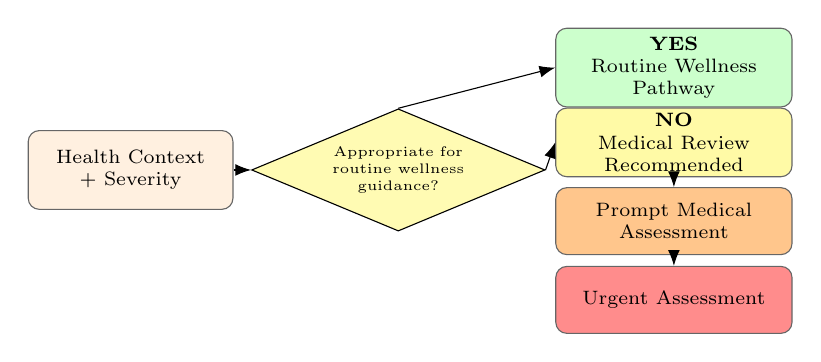
\begin{tikzpicture}[>=Latex]
\node[draw=black!60,rounded corners,fill=orange!12,minimum width=2.6cm,minimum height=1.0cm,align=center,font=\scriptsize,text width=2.35cm,inner sep=2pt] (s12_ctx) at (0,0) {Health Context\\+ Severity};
\node[draw,diamond,aspect=2.4,fill=yellow!30,align=center,font=\tiny,text width=2.1cm,inner sep=1pt] (s12_d) at (3.4,0) {Appropriate for\\routine wellness\\guidance?};
\draw[-{Latex[length=2mm]}] (s12_ctx.east)--(s12_d.west);
\node[draw=black!60,rounded corners,fill=green!20,minimum width=3.0cm,minimum height=1.0cm,align=center,font=\scriptsize,text width=2.75cm,inner sep=2pt] (s12_yes) at (6.9,1.3) {\textbf{YES}\\Routine Wellness\\Pathway};
\draw[-{Latex[length=2mm]}] (s12_d.north)--(s12_yes.west);
\node[draw=black!60,rounded corners,fill=yellow!35,minimum width=3.0cm,minimum height=0.85cm,align=center,font=\scriptsize,text width=2.75cm,inner sep=2pt] (s12_n1) at (6.9,0.35) {\textbf{NO}\\Medical Review\\Recommended};
\node[draw=black!60,rounded corners,fill=orange!45,minimum width=3.0cm,minimum height=0.85cm,align=center,font=\scriptsize,text width=2.75cm,inner sep=2pt] (s12_n2) at (6.9,-0.65) {Prompt Medical\\Assessment};
\node[draw=black!60,rounded corners,fill=red!45,minimum width=3.0cm,minimum height=0.85cm,align=center,font=\scriptsize,text width=2.75cm,inner sep=2pt] (s12_n3) at (6.9,-1.65) {Urgent Assessment};
\draw[-{Latex[length=2mm]}] (s12_d.east)--(s12_n1.west);
\draw[-{Latex[length=2mm]}] (s12_n1.south)--(s12_n2.north);
\draw[-{Latex[length=2mm]}] (s12_n2.south)--(s12_n3.north);
\end{tikzpicture}
\end{adjustbox}
\end{center}
\end{frame}

\begin{frame}{Module 12: Safety and Referral Engine}
\textcolor{black!55}{\scriptsize Schematic 2 -- Input / Output relations}\\[2pt]
\begin{center}
\begin{adjustbox}{max width=0.96\linewidth,max height=0.66\textheight}
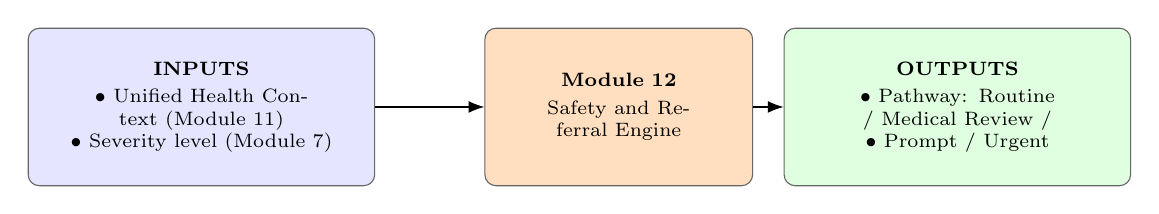
\begin{tikzpicture}[>=Latex]
\node[draw=black!60,rounded corners,fill=blue!10,minimum width=4.4cm,minimum height=2.0cm,align=center,font=\scriptsize,text width=4.15cm,inner sep=2pt] (io_in) at (0,0) {\textbf{\scriptsize INPUTS}\\[2pt]$\bullet$ Unified Health Context (Module 11)\\$\bullet$ Severity level (Module 7)};
\node[draw=black!60,rounded corners,fill=orange!25,minimum width=3.4cm,minimum height=2.0cm,align=center,font=\scriptsize,text width=3.15cm,inner sep=2pt] (io_p) at (5.3,0) {\textbf{Module 12}\\[2pt]Safety and Referral Engine};
\node[draw=black!60,rounded corners,fill=green!12,minimum width=4.4cm,minimum height=2.0cm,align=center,font=\scriptsize,text width=4.15cm,inner sep=2pt] (io_out) at (9.6,0) {\textbf{\scriptsize OUTPUTS}\\[2pt]$\bullet$ Pathway: Routine / Medical Review /\\$\bullet$ Prompt / Urgent};
\draw[-{Latex[length=2mm]}] (io_in.east)--(io_p.west);
\draw[-{Latex[length=2mm]}] (io_p.east)--(io_out.west);
\end{tikzpicture}
\end{adjustbox}
\end{center}
\end{frame}

\begin{frame}{Module 13: Priority Engine}
\textcolor{black!55}{\scriptsize Cluster 5 -- \textcolor{red}{\textbf{Safety \& Priority}} (M12--M14)}\\[2pt]
\begin{columns}[T,onlytextwidth]
\begin{column}{0.5\textwidth}
\begin{tcolorbox}[colback=blue!7,colframe=blue!55!black,title=\textbf{Motivation},boxrule=0.6pt,arc=1mm,left=5pt,right=5pt,top=3pt,bottom=3pt,fonttitle=\small]
\footnotesize Six abnormal findings should not produce six competing recommendations.
\end{tcolorbox}
\vspace{5pt}
\begin{tcolorbox}[colback=teal!7,colframe=teal!55!black,title=\textbf{Method},boxrule=0.6pt,arc=1mm,left=5pt,right=5pt,top=3pt,bottom=3pt,fonttitle=\small]
\footnotesize Group related findings and identify the upstream priorities that explain the most downstream issues.
\end{tcolorbox}
\end{column}
\begin{column}{0.5\textwidth}
\begin{tcolorbox}[colback=green!8,colframe=green!45!black,title=\textbf{Result},boxrule=0.6pt,arc=1mm,left=5pt,right=5pt,top=3pt,bottom=3pt,fonttitle=\small]
\footnotesize A short, ranked priority list (typically 3--4 items) instead of a flat finding list.
\end{tcolorbox}
\vspace{5pt}
\begin{tcolorbox}[colback=orange!10,colframe=orange!65!black,title=\textbf{Conclusion},boxrule=0.6pt,arc=1mm,left=5pt,right=5pt,top=3pt,bottom=3pt,fonttitle=\small]
\footnotesize Grouping before recommending is what keeps the final report usable.
\end{tcolorbox}
\end{column}
\end{columns}
\end{frame}

\begin{frame}{Module 13: Priority Engine}
\textcolor{black!55}{\scriptsize Schematic 1 -- Many findings converge into a few priorities}\\[2pt]
\begin{center}
\begin{adjustbox}{max width=0.96\linewidth,max height=0.66\textheight}
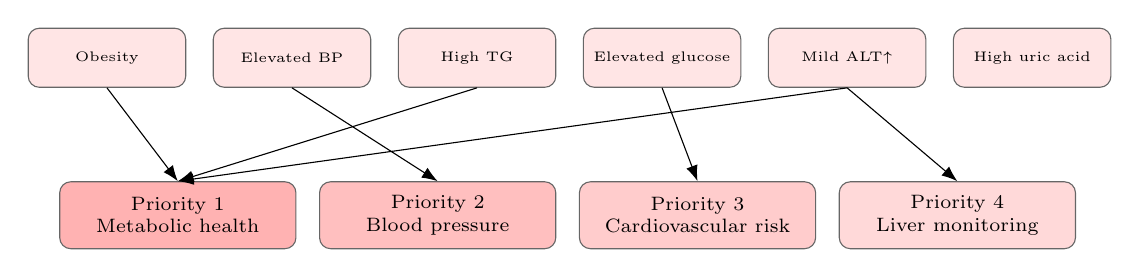
\begin{tikzpicture}[>=Latex]
\node[draw=black!60,rounded corners,fill=red!10,minimum width=2.0cm,minimum height=0.75cm,align=center,font=\tiny,text width=1.75cm,inner sep=2pt] (g0) at (0.0,0.0) {Obesity};
\node[draw=black!60,rounded corners,fill=red!10,minimum width=2.0cm,minimum height=0.75cm,align=center,font=\tiny,text width=1.75cm,inner sep=2pt] (g1) at (2.35,0.0) {Elevated BP};
\node[draw=black!60,rounded corners,fill=red!10,minimum width=2.0cm,minimum height=0.75cm,align=center,font=\tiny,text width=1.75cm,inner sep=2pt] (g2) at (4.7,0.0) {High TG};
\node[draw=black!60,rounded corners,fill=red!10,minimum width=2.0cm,minimum height=0.75cm,align=center,font=\tiny,text width=1.75cm,inner sep=2pt] (g3) at (7.050000000000001,0.0) {Elevated glucose};
\node[draw=black!60,rounded corners,fill=red!10,minimum width=2.0cm,minimum height=0.75cm,align=center,font=\tiny,text width=1.75cm,inner sep=2pt] (g4) at (9.4,0.0) {Mild ALT$\uparrow$};
\node[draw=black!60,rounded corners,fill=red!10,minimum width=2.0cm,minimum height=0.75cm,align=center,font=\tiny,text width=1.75cm,inner sep=2pt] (g5) at (11.75,0.0) {High uric acid};
\node[draw=black!60,rounded corners,fill=red!30,minimum width=3.0cm,minimum height=0.85cm,align=center,font=\scriptsize,text width=2.75cm,inner sep=2pt] (pr1) at (0.9,-2.0) {Priority 1\\Metabolic health};
\node[draw=black!60,rounded corners,fill=red!25,minimum width=3.0cm,minimum height=0.85cm,align=center,font=\scriptsize,text width=2.75cm,inner sep=2pt] (pr2) at (4.2,-2.0) {Priority 2\\Blood pressure};
\node[draw=black!60,rounded corners,fill=red!20,minimum width=3.0cm,minimum height=0.85cm,align=center,font=\scriptsize,text width=2.75cm,inner sep=2pt] (pr3) at (7.5,-2.0) {Priority 3\\Cardiovascular risk};
\node[draw=black!60,rounded corners,fill=red!15,minimum width=3.0cm,minimum height=0.85cm,align=center,font=\scriptsize,text width=2.75cm,inner sep=2pt] (pr4) at (10.8,-2.0) {Priority 4\\Liver monitoring};
\draw[-{Latex[length=2mm]}] (g0.south)--(pr1.north);
\draw[-{Latex[length=2mm]}] (g2.south)--(pr1.north);
\draw[-{Latex[length=2mm]}] (g4.south)--(pr1.north);
\draw[-{Latex[length=2mm]}] (g1.south)--(pr2.north);
\draw[-{Latex[length=2mm]}] (g3.south)--(pr3.north);
\draw[-{Latex[length=2mm]}] (g4.south)--(pr4.north);
\end{tikzpicture}
\end{adjustbox}
\end{center}
\end{frame}

\begin{frame}{Module 13: Priority Engine}
\textcolor{black!55}{\scriptsize Schematic 2 -- Input / Output relations}\\[2pt]
\begin{center}
\begin{adjustbox}{max width=0.96\linewidth,max height=0.66\textheight}
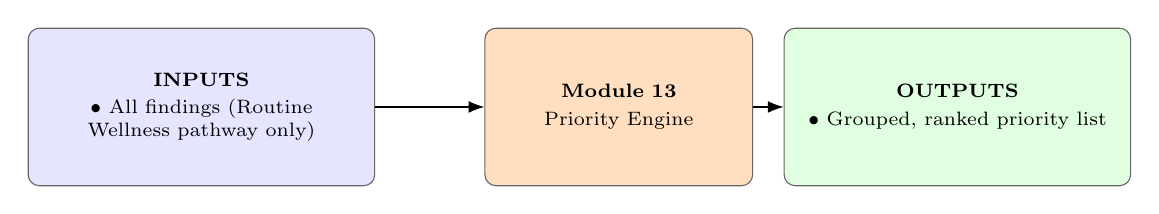
\begin{tikzpicture}[>=Latex]
\node[draw=black!60,rounded corners,fill=blue!10,minimum width=4.4cm,minimum height=2.0cm,align=center,font=\scriptsize,text width=4.15cm,inner sep=2pt] (io_in) at (0,0) {\textbf{\scriptsize INPUTS}\\[2pt]$\bullet$ All findings (Routine Wellness pathway only)};
\node[draw=black!60,rounded corners,fill=orange!25,minimum width=3.4cm,minimum height=2.0cm,align=center,font=\scriptsize,text width=3.15cm,inner sep=2pt] (io_p) at (5.3,0) {\textbf{Module 13}\\[2pt]Priority Engine};
\node[draw=black!60,rounded corners,fill=green!12,minimum width=4.4cm,minimum height=2.0cm,align=center,font=\scriptsize,text width=4.15cm,inner sep=2pt] (io_out) at (9.6,0) {\textbf{\scriptsize OUTPUTS}\\[2pt]$\bullet$ Grouped, ranked priority list};
\draw[-{Latex[length=2mm]}] (io_in.east)--(io_p.west);
\draw[-{Latex[length=2mm]}] (io_p.east)--(io_out.west);
\end{tikzpicture}
\end{adjustbox}
\end{center}
\end{frame}

\begin{frame}{Module 14: Root-Factor Mapping}
\textcolor{black!55}{\scriptsize Cluster 5 -- \textcolor{red}{\textbf{Safety \& Priority}} (M12--M14)}\\[2pt]
\begin{columns}[T,onlytextwidth]
\begin{column}{0.5\textwidth}
\begin{tcolorbox}[colback=blue!7,colframe=blue!55!black,title=\textbf{Motivation},boxrule=0.6pt,arc=1mm,left=5pt,right=5pt,top=3pt,bottom=3pt,fonttitle=\small]
\footnotesize Treating five metabolic abnormalities as five separate problems obscures their shared cause.
\end{tcolorbox}
\vspace{5pt}
\begin{tcolorbox}[colback=teal!7,colframe=teal!55!black,title=\textbf{Method},boxrule=0.6pt,arc=1mm,left=5pt,right=5pt,top=3pt,bottom=3pt,fonttitle=\small]
\footnotesize Trace findings back to modifiable upstream factors (e.g. excess weight $\to$ insulin resistance $\to$ multiple markers).
\end{tcolorbox}
\end{column}
\begin{column}{0.5\textwidth}
\begin{tcolorbox}[colback=green!8,colframe=green!45!black,title=\textbf{Result},boxrule=0.6pt,arc=1mm,left=5pt,right=5pt,top=3pt,bottom=3pt,fonttitle=\small]
\footnotesize A causal chain the report can state explicitly to the user.
\end{tcolorbox}
\vspace{5pt}
\begin{tcolorbox}[colback=orange!10,colframe=orange!65!black,title=\textbf{Conclusion},boxrule=0.6pt,arc=1mm,left=5pt,right=5pt,top=3pt,bottom=3pt,fonttitle=\small]
\footnotesize One well-chosen intervention can be shown to improve several findings at once.
\end{tcolorbox}
\end{column}
\end{columns}
\end{frame}

\begin{frame}{Module 14: Root-Factor Mapping}
\textcolor{black!55}{\scriptsize Schematic 1 -- One upstream factor, five downstream effects}\\[2pt]
\begin{center}
\begin{adjustbox}{max width=0.96\linewidth,max height=0.66\textheight}
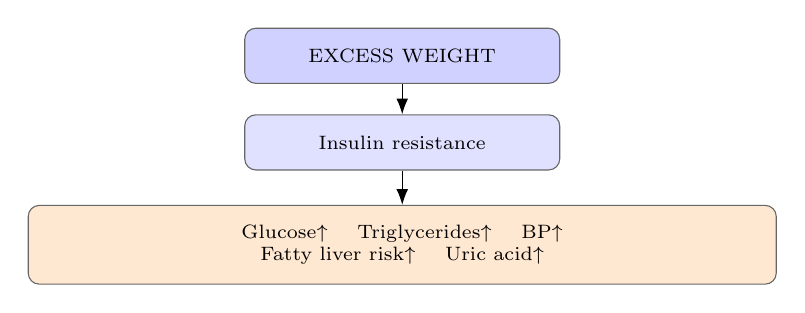
\begin{tikzpicture}[>=Latex]
\node[draw=black!60,rounded corners,fill=blue!18,minimum width=4.0cm,minimum height=0.7cm,align=center,font=\scriptsize,text width=3.75cm,inner sep=2pt] (rf1) at (0,1.2) {EXCESS WEIGHT};
\node[draw=black!60,rounded corners,fill=blue!12,minimum width=4.0cm,minimum height=0.7cm,align=center,font=\scriptsize,text width=3.75cm,inner sep=2pt] (rf2) at (0,0.1) {Insulin resistance};
\draw[-{Latex[length=2mm]}] (rf1.south)--(rf2.north);
\node[draw=black!60,rounded corners,fill=orange!18,minimum width=9.5cm,minimum height=1.0cm,align=center,font=\scriptsize,text width=9.25cm,inner sep=2pt] (rf3) at (0,-1.2) {Glucose$\uparrow$ \quad Triglycerides$\uparrow$ \quad BP$\uparrow$\\Fatty liver risk$\uparrow$ \quad Uric acid$\uparrow$};
\draw[-{Latex[length=2mm]}] (rf2.south)--(rf3.north);
\end{tikzpicture}
\end{adjustbox}
\end{center}
\end{frame}

\begin{frame}{Module 14: Root-Factor Mapping}
\textcolor{black!55}{\scriptsize Schematic 2 -- Input / Output relations}\\[2pt]
\begin{center}
\begin{adjustbox}{max width=0.96\linewidth,max height=0.66\textheight}
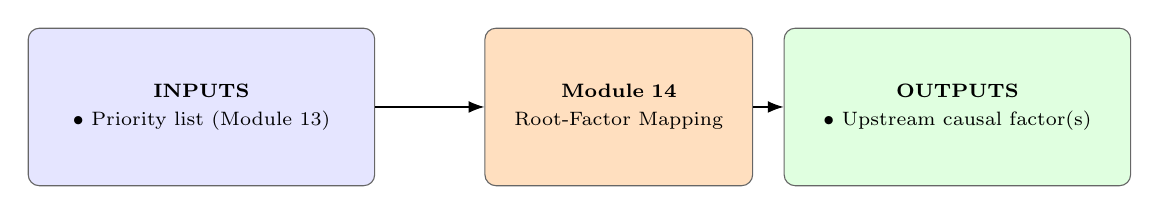
\begin{tikzpicture}[>=Latex]
\node[draw=black!60,rounded corners,fill=blue!10,minimum width=4.4cm,minimum height=2.0cm,align=center,font=\scriptsize,text width=4.15cm,inner sep=2pt] (io_in) at (0,0) {\textbf{\scriptsize INPUTS}\\[2pt]$\bullet$ Priority list (Module 13)};
\node[draw=black!60,rounded corners,fill=orange!25,minimum width=3.4cm,minimum height=2.0cm,align=center,font=\scriptsize,text width=3.15cm,inner sep=2pt] (io_p) at (5.3,0) {\textbf{Module 14}\\[2pt]Root-Factor Mapping};
\node[draw=black!60,rounded corners,fill=green!12,minimum width=4.4cm,minimum height=2.0cm,align=center,font=\scriptsize,text width=4.15cm,inner sep=2pt] (io_out) at (9.6,0) {\textbf{\scriptsize OUTPUTS}\\[2pt]$\bullet$ Upstream causal factor(s)};
\draw[-{Latex[length=2mm]}] (io_in.east)--(io_p.west);
\draw[-{Latex[length=2mm]}] (io_p.east)--(io_out.west);
\end{tikzpicture}
\end{adjustbox}
\end{center}
\end{frame}

\section{Cluster 6 -- Recommendation \& Explanation (M15--M18)}

\begin{frame}{19. Recommendation Structure}
\begin{columns}[T,onlytextwidth]
\begin{column}{0.5\textwidth}
\begin{tcolorbox}[colback=blue!7,colframe=blue!55!black,title=\textbf{Motivation},boxrule=0.6pt,arc=1mm,left=5pt,right=5pt,top=3pt,bottom=3pt,fonttitle=\small]
\footnotesize A recommendation without a fixed schema will vary in quality and completeness across cases.
\end{tcolorbox}
\vspace{5pt}
\begin{tcolorbox}[colback=teal!7,colframe=teal!55!black,title=\textbf{Method},boxrule=0.6pt,arc=1mm,left=5pt,right=5pt,top=3pt,bottom=3pt,fonttitle=\small]
\footnotesize Require seven fields on every recommendation: trigger, health issue, recommendation, why, expected benefit, precaution, follow-up.
\end{tcolorbox}
\end{column}
\begin{column}{0.5\textwidth}
\begin{tcolorbox}[colback=green!8,colframe=green!45!black,title=\textbf{Result},boxrule=0.6pt,arc=1mm,left=5pt,right=5pt,top=3pt,bottom=3pt,fonttitle=\small]
\footnotesize A worked example (triglycerides + weight) showing the schema fully populated.
\end{tcolorbox}
\vspace{5pt}
\begin{tcolorbox}[colback=orange!10,colframe=orange!65!black,title=\textbf{Conclusion},boxrule=0.6pt,arc=1mm,left=5pt,right=5pt,top=3pt,bottom=3pt,fonttitle=\small]
\footnotesize This schema is what Modules 15--18 all read from and write to.
\end{tcolorbox}
\end{column}
\end{columns}
\end{frame}

\begin{frame}{19. Recommendation Structure}
\textcolor{black!55}{\scriptsize Seven-field recommendation schema, with a worked example}\\[2pt]
\begin{center}
\begin{adjustbox}{max width=0.96\linewidth,max height=0.66\textheight}
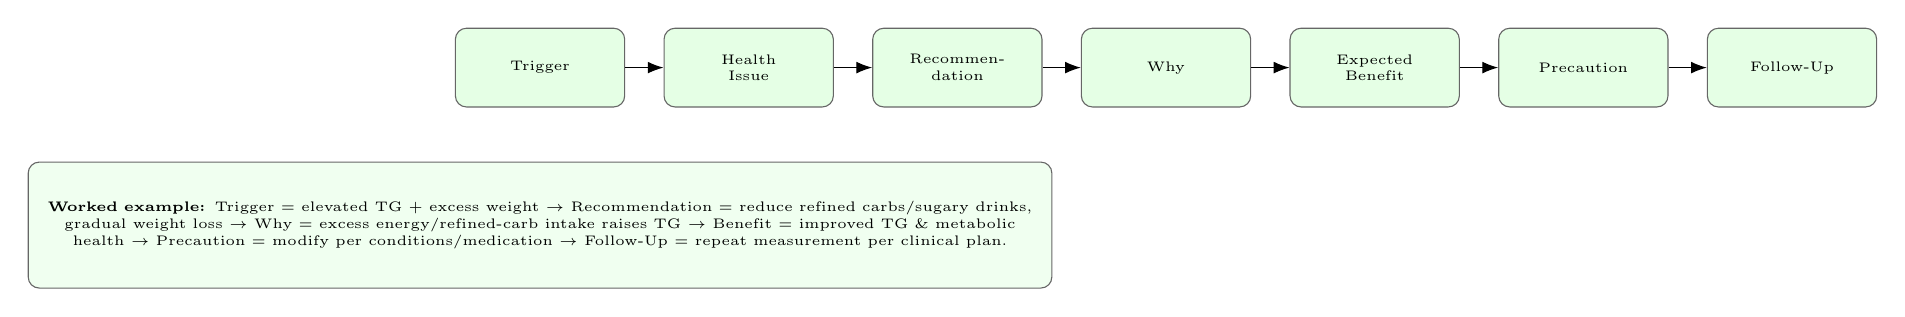
\begin{tikzpicture}[>=Latex]
\node[draw=black!60,rounded corners,fill=green!10,minimum width=2.15cm,minimum height=1.0cm,align=center,font=\tiny,text width=1.9cm,inner sep=2pt] (h0) at (0,0) {Trigger};
\node[draw=black!60,rounded corners,fill=green!10,minimum width=2.15cm,minimum height=1.0cm,align=center,font=\tiny,text width=1.9cm,inner sep=2pt] (h1) at (2.65,0) {Health\\Issue};
\node[draw=black!60,rounded corners,fill=green!10,minimum width=2.15cm,minimum height=1.0cm,align=center,font=\tiny,text width=1.9cm,inner sep=2pt] (h2) at (5.3,0) {Recommen-\\dation};
\node[draw=black!60,rounded corners,fill=green!10,minimum width=2.15cm,minimum height=1.0cm,align=center,font=\tiny,text width=1.9cm,inner sep=2pt] (h3) at (7.949999999999999,0) {Why};
\node[draw=black!60,rounded corners,fill=green!10,minimum width=2.15cm,minimum height=1.0cm,align=center,font=\tiny,text width=1.9cm,inner sep=2pt] (h4) at (10.6,0) {Expected\\Benefit};
\node[draw=black!60,rounded corners,fill=green!10,minimum width=2.15cm,minimum height=1.0cm,align=center,font=\tiny,text width=1.9cm,inner sep=2pt] (h5) at (13.25,0) {Precaution};
\node[draw=black!60,rounded corners,fill=green!10,minimum width=2.15cm,minimum height=1.0cm,align=center,font=\tiny,text width=1.9cm,inner sep=2pt] (h6) at (15.9,0) {Follow-Up};
\draw[-{Latex[length=2mm]}] (h0.east)--(h1.west);
\draw[-{Latex[length=2mm]}] (h1.east)--(h2.west);
\draw[-{Latex[length=2mm]}] (h2.east)--(h3.west);
\draw[-{Latex[length=2mm]}] (h3.east)--(h4.west);
\draw[-{Latex[length=2mm]}] (h4.east)--(h5.west);
\draw[-{Latex[length=2mm]}] (h5.east)--(h6.west);
\node[draw=black!60,rounded corners,fill=green!6,minimum width=13.0cm,minimum height=1.6cm,align=center,font=\tiny,text width=12.75cm,inner sep=2pt] (rex) at (0,-2.0) {\textbf{Worked example:} Trigger = elevated TG + excess weight $\to$ Recommendation = reduce refined carbs/sugary drinks, gradual weight loss $\to$ Why = excess energy/refined-carb intake raises TG $\to$ Benefit = improved TG \& metabolic health $\to$ Precaution = modify per conditions/medication $\to$ Follow-Up = repeat measurement per clinical plan.};
\end{tikzpicture}
\end{adjustbox}
\end{center}
\end{frame}

\begin{frame}{Module 15: Wellness Recommendation Engine}
\textcolor{black!55}{\scriptsize Cluster 6 -- \textcolor{green!60!black}{\textbf{Recommendation \& Explanation}} (M15--M18)}\\[2pt]
\begin{columns}[T,onlytextwidth]
\begin{column}{0.5\textwidth}
\begin{tcolorbox}[colback=blue!7,colframe=blue!55!black,title=\textbf{Motivation},boxrule=0.6pt,arc=1mm,left=5pt,right=5pt,top=3pt,bottom=3pt,fonttitle=\small]
\footnotesize Recommendations need a bounded, evidence-proportionate scope for Version 1.
\end{tcolorbox}
\vspace{5pt}
\begin{tcolorbox}[colback=teal!7,colframe=teal!55!black,title=\textbf{Method},boxrule=0.6pt,arc=1mm,left=5pt,right=5pt,top=3pt,bottom=3pt,fonttitle=\small]
\footnotesize Draw candidate recommendations from nine lifestyle domains, proportional to the evidence available.
\end{tcolorbox}
\end{column}
\begin{column}{0.5\textwidth}
\begin{tcolorbox}[colback=green!8,colframe=green!45!black,title=\textbf{Result},boxrule=0.6pt,arc=1mm,left=5pt,right=5pt,top=3pt,bottom=3pt,fonttitle=\small]
\footnotesize A candidate recommendation set tied to specific triggers.
\end{tcolorbox}
\vspace{5pt}
\begin{tcolorbox}[colback=orange!10,colframe=orange!65!black,title=\textbf{Conclusion},boxrule=0.6pt,arc=1mm,left=5pt,right=5pt,top=3pt,bottom=3pt,fonttitle=\small]
\footnotesize Scope discipline keeps Version 1 focused on what wellness guidance can responsibly claim.
\end{tcolorbox}
\end{column}
\end{columns}
\end{frame}

\begin{frame}{Module 15: Wellness Recommendation Engine}
\textcolor{black!55}{\scriptsize Schematic 1 -- Nine bounded recommendation domains}\\[2pt]
\begin{center}
\begin{adjustbox}{max width=0.96\linewidth,max height=0.66\textheight}
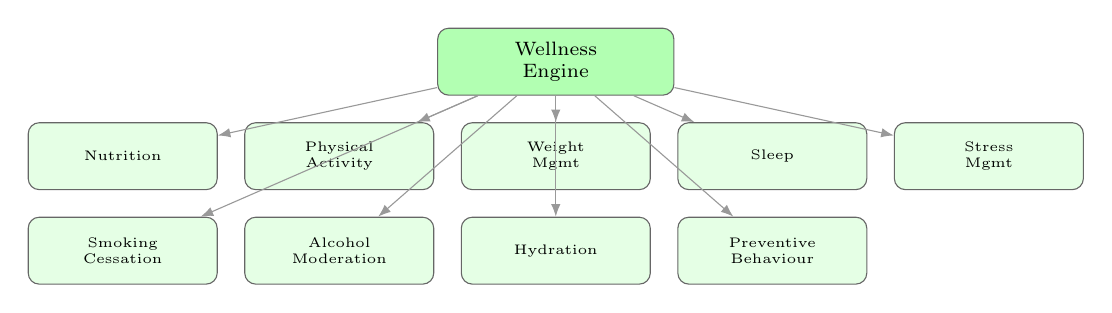
\begin{tikzpicture}[>=Latex]
\node[draw=black!60,rounded corners,fill=green!10,minimum width=2.4cm,minimum height=0.85cm,align=center,font=\tiny,text width=2.15cm,inner sep=2pt] (g0) at (0.0,0.0) {Nutrition};
\node[draw=black!60,rounded corners,fill=green!10,minimum width=2.4cm,minimum height=0.85cm,align=center,font=\tiny,text width=2.15cm,inner sep=2pt] (g1) at (2.75,0.0) {Physical\\Activity};
\node[draw=black!60,rounded corners,fill=green!10,minimum width=2.4cm,minimum height=0.85cm,align=center,font=\tiny,text width=2.15cm,inner sep=2pt] (g2) at (5.5,0.0) {Weight\\Mgmt};
\node[draw=black!60,rounded corners,fill=green!10,minimum width=2.4cm,minimum height=0.85cm,align=center,font=\tiny,text width=2.15cm,inner sep=2pt] (g3) at (8.25,0.0) {Sleep};
\node[draw=black!60,rounded corners,fill=green!10,minimum width=2.4cm,minimum height=0.85cm,align=center,font=\tiny,text width=2.15cm,inner sep=2pt] (g4) at (11.0,0.0) {Stress\\Mgmt};
\node[draw=black!60,rounded corners,fill=green!10,minimum width=2.4cm,minimum height=0.85cm,align=center,font=\tiny,text width=2.15cm,inner sep=2pt] (g5) at (0.0,-1.2) {Smoking\\Cessation};
\node[draw=black!60,rounded corners,fill=green!10,minimum width=2.4cm,minimum height=0.85cm,align=center,font=\tiny,text width=2.15cm,inner sep=2pt] (g6) at (2.75,-1.2) {Alcohol\\Moderation};
\node[draw=black!60,rounded corners,fill=green!10,minimum width=2.4cm,minimum height=0.85cm,align=center,font=\tiny,text width=2.15cm,inner sep=2pt] (g7) at (5.5,-1.2) {Hydration};
\node[draw=black!60,rounded corners,fill=green!10,minimum width=2.4cm,minimum height=0.85cm,align=center,font=\tiny,text width=2.15cm,inner sep=2pt] (g8) at (8.25,-1.2) {Preventive\\Behaviour};
\node[draw=black!60,rounded corners,fill=green!30,minimum width=3.0cm,minimum height=0.85cm,align=center,font=\scriptsize,text width=2.75cm,inner sep=2pt] (gc) at (5.5,1.2) {Wellness\\Engine};
\draw[-{Latex[length=1.6mm]},black!40] (gc)--(g0);
\draw[-{Latex[length=1.6mm]},black!40] (gc)--(g1);
\draw[-{Latex[length=1.6mm]},black!40] (gc)--(g2);
\draw[-{Latex[length=1.6mm]},black!40] (gc)--(g3);
\draw[-{Latex[length=1.6mm]},black!40] (gc)--(g4);
\draw[-{Latex[length=1.6mm]},black!40] (gc)--(g5);
\draw[-{Latex[length=1.6mm]},black!40] (gc)--(g6);
\draw[-{Latex[length=1.6mm]},black!40] (gc)--(g7);
\draw[-{Latex[length=1.6mm]},black!40] (gc)--(g8);
\end{tikzpicture}
\end{adjustbox}
\end{center}
\end{frame}

\begin{frame}{Module 15: Wellness Recommendation Engine}
\textcolor{black!55}{\scriptsize Schematic 2 -- Input / Output relations}\\[2pt]
\begin{center}
\begin{adjustbox}{max width=0.96\linewidth,max height=0.66\textheight}
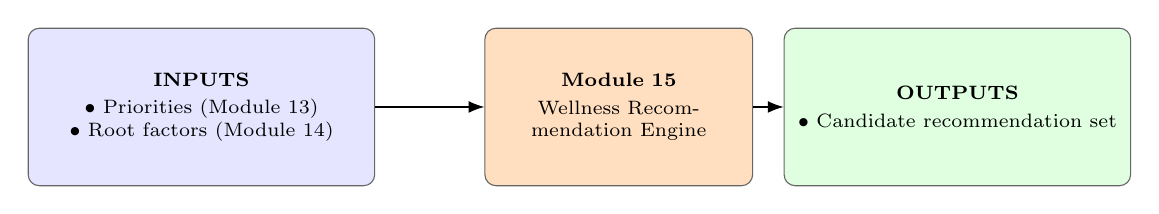
\begin{tikzpicture}[>=Latex]
\node[draw=black!60,rounded corners,fill=blue!10,minimum width=4.4cm,minimum height=2.0cm,align=center,font=\scriptsize,text width=4.15cm,inner sep=2pt] (io_in) at (0,0) {\textbf{\scriptsize INPUTS}\\[2pt]$\bullet$ Priorities (Module 13)\\$\bullet$ Root factors (Module 14)};
\node[draw=black!60,rounded corners,fill=orange!25,minimum width=3.4cm,minimum height=2.0cm,align=center,font=\scriptsize,text width=3.15cm,inner sep=2pt] (io_p) at (5.3,0) {\textbf{Module 15}\\[2pt]Wellness Recommendation Engine};
\node[draw=black!60,rounded corners,fill=green!12,minimum width=4.4cm,minimum height=2.0cm,align=center,font=\scriptsize,text width=4.15cm,inner sep=2pt] (io_out) at (9.6,0) {\textbf{\scriptsize OUTPUTS}\\[2pt]$\bullet$ Candidate recommendation set};
\draw[-{Latex[length=2mm]}] (io_in.east)--(io_p.west);
\draw[-{Latex[length=2mm]}] (io_p.east)--(io_out.west);
\end{tikzpicture}
\end{adjustbox}
\end{center}
\end{frame}

\begin{frame}{Module 16: Recommendation Conflict Resolver}
\textcolor{black!55}{\scriptsize Cluster 6 -- \textcolor{green!60!black}{\textbf{Recommendation \& Explanation}} (M15--M18)}\\[2pt]
\begin{columns}[T,onlytextwidth]
\begin{column}{0.5\textwidth}
\begin{tcolorbox}[colback=blue!7,colframe=blue!55!black,title=\textbf{Motivation},boxrule=0.6pt,arc=1mm,left=5pt,right=5pt,top=3pt,bottom=3pt,fonttitle=\small]
\footnotesize A generically sound recommendation can be actively harmful in the wrong patient context.
\end{tcolorbox}
\vspace{5pt}
\begin{tcolorbox}[colback=teal!7,colframe=teal!55!black,title=\textbf{Method},boxrule=0.6pt,arc=1mm,left=5pt,right=5pt,top=3pt,bottom=3pt,fonttitle=\small]
\footnotesize Pass every candidate recommendation through known conflict rules before it is displayed.
\end{tcolorbox}
\end{column}
\begin{column}{0.5\textwidth}
\begin{tcolorbox}[colback=green!8,colframe=green!45!black,title=\textbf{Result},boxrule=0.6pt,arc=1mm,left=5pt,right=5pt,top=3pt,bottom=3pt,fonttitle=\small]
\footnotesize Recommendations are suppressed or modified whenever a contraindication applies.
\end{tcolorbox}
\vspace{5pt}
\begin{tcolorbox}[colback=orange!10,colframe=orange!65!black,title=\textbf{Conclusion},boxrule=0.6pt,arc=1mm,left=5pt,right=5pt,top=3pt,bottom=3pt,fonttitle=\small]
\footnotesize No recommendation reaches the user without first surviving a safety check.
\end{tcolorbox}
\end{column}
\end{columns}
\end{frame}

\begin{frame}{Module 16: Recommendation Conflict Resolver}
\textcolor{black!55}{\scriptsize Schematic 1 -- Three worked conflict-check examples}\\[2pt]
\begin{center}
\begin{adjustbox}{max width=0.96\linewidth,max height=0.66\textheight}
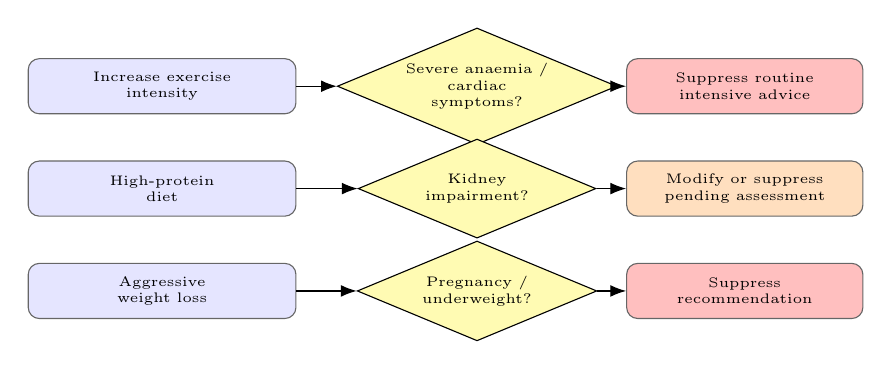
\begin{tikzpicture}[>=Latex]
\node[draw=black!60,rounded corners,fill=blue!10,minimum width=3.4cm,minimum height=0.7cm,align=center,font=\tiny,text width=3.15cm,inner sep=2pt] (cf1a) at (0,1.6) {Increase exercise\\intensity};
\node[draw,diamond,aspect=2.4,fill=yellow!30,align=center,font=\tiny,text width=1.9cm,inner sep=1pt] (cf1d) at (4.0,1.6) {Severe anaemia /\\cardiac symptoms?};
\node[draw=black!60,rounded corners,fill=red!25,minimum width=3.0cm,minimum height=0.7cm,align=center,font=\tiny,text width=2.75cm,inner sep=2pt] (cf1o) at (7.4,1.6) {Suppress routine\\intensive advice};
\draw[-{Latex[length=2mm]}] (cf1a.east)--(cf1d.west);
\draw[-{Latex[length=2mm]}] (cf1d.east)--(cf1o.west);
\node[draw=black!60,rounded corners,fill=blue!10,minimum width=3.4cm,minimum height=0.7cm,align=center,font=\tiny,text width=3.15cm,inner sep=2pt] (cf2a) at (0,0.3) {High-protein\\diet};
\node[draw,diamond,aspect=2.4,fill=yellow!30,align=center,font=\tiny,text width=1.9cm,inner sep=1pt] (cf2d) at (4.0,0.3) {Kidney\\impairment?};
\node[draw=black!60,rounded corners,fill=orange!25,minimum width=3.0cm,minimum height=0.7cm,align=center,font=\tiny,text width=2.75cm,inner sep=2pt] (cf2o) at (7.4,0.3) {Modify or suppress\\pending assessment};
\draw[-{Latex[length=2mm]}] (cf2a.east)--(cf2d.west);
\draw[-{Latex[length=2mm]}] (cf2d.east)--(cf2o.west);
\node[draw=black!60,rounded corners,fill=blue!10,minimum width=3.4cm,minimum height=0.7cm,align=center,font=\tiny,text width=3.15cm,inner sep=2pt] (cf3a) at (0,-1.0) {Aggressive\\weight loss};
\node[draw,diamond,aspect=2.4,fill=yellow!30,align=center,font=\tiny,text width=1.9cm,inner sep=1pt] (cf3d) at (4.0,-1.0) {Pregnancy /\\underweight?};
\node[draw=black!60,rounded corners,fill=red!25,minimum width=3.0cm,minimum height=0.7cm,align=center,font=\tiny,text width=2.75cm,inner sep=2pt] (cf3o) at (7.4,-1.0) {Suppress\\recommendation};
\draw[-{Latex[length=2mm]}] (cf3a.east)--(cf3d.west);
\draw[-{Latex[length=2mm]}] (cf3d.east)--(cf3o.west);
\end{tikzpicture}
\end{adjustbox}
\end{center}
\end{frame}

\begin{frame}{Module 16: Recommendation Conflict Resolver}
\textcolor{black!55}{\scriptsize Schematic 2 -- Input / Output relations}\\[2pt]
\begin{center}
\begin{adjustbox}{max width=0.96\linewidth,max height=0.66\textheight}
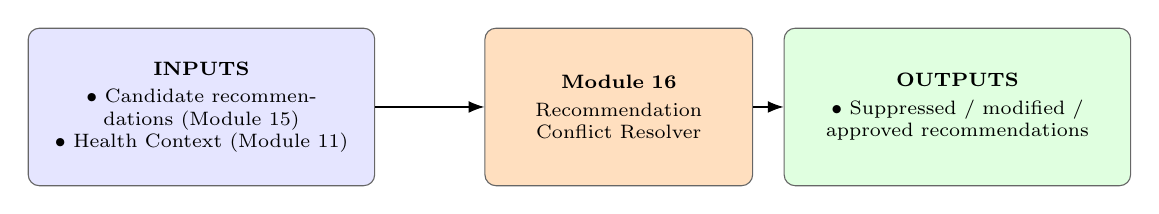
\begin{tikzpicture}[>=Latex]
\node[draw=black!60,rounded corners,fill=blue!10,minimum width=4.4cm,minimum height=2.0cm,align=center,font=\scriptsize,text width=4.15cm,inner sep=2pt] (io_in) at (0,0) {\textbf{\scriptsize INPUTS}\\[2pt]$\bullet$ Candidate recommendations (Module 15)\\$\bullet$ Health Context (Module 11)};
\node[draw=black!60,rounded corners,fill=orange!25,minimum width=3.4cm,minimum height=2.0cm,align=center,font=\scriptsize,text width=3.15cm,inner sep=2pt] (io_p) at (5.3,0) {\textbf{Module 16}\\[2pt]Recommendation Conflict Resolver};
\node[draw=black!60,rounded corners,fill=green!12,minimum width=4.4cm,minimum height=2.0cm,align=center,font=\scriptsize,text width=4.15cm,inner sep=2pt] (io_out) at (9.6,0) {\textbf{\scriptsize OUTPUTS}\\[2pt]$\bullet$ Suppressed / modified / approved recommendations};
\draw[-{Latex[length=2mm]}] (io_in.east)--(io_p.west);
\draw[-{Latex[length=2mm]}] (io_p.east)--(io_out.west);
\end{tikzpicture}
\end{adjustbox}
\end{center}
\end{frame}

\begin{frame}{Module 17: Recommendation Priority System}
\textcolor{black!55}{\scriptsize Cluster 6 -- \textcolor{green!60!black}{\textbf{Recommendation \& Explanation}} (M15--M18)}\\[2pt]
\begin{columns}[T,onlytextwidth]
\begin{column}{0.5\textwidth}
\begin{tcolorbox}[colback=blue!7,colframe=blue!55!black,title=\textbf{Motivation},boxrule=0.6pt,arc=1mm,left=5pt,right=5pt,top=3pt,bottom=3pt,fonttitle=\small]
\footnotesize A patient handed ten equally-weighted actions acts on none of them.
\end{tcolorbox}
\vspace{5pt}
\begin{tcolorbox}[colback=teal!7,colframe=teal!55!black,title=\textbf{Method},boxrule=0.6pt,arc=1mm,left=5pt,right=5pt,top=3pt,bottom=3pt,fonttitle=\small]
\footnotesize Score each surviving recommendation on six factors: importance, modifiability, findings affected, safety, benefit, feasibility.
\end{tcolorbox}
\end{column}
\begin{column}{0.5\textwidth}
\begin{tcolorbox}[colback=green!8,colframe=green!45!black,title=\textbf{Result},boxrule=0.6pt,arc=1mm,left=5pt,right=5pt,top=3pt,bottom=3pt,fonttitle=\small]
\footnotesize Roughly three main priorities, with secondary items underneath.
\end{tcolorbox}
\vspace{5pt}
\begin{tcolorbox}[colback=orange!10,colframe=orange!65!black,title=\textbf{Conclusion},boxrule=0.6pt,arc=1mm,left=5pt,right=5pt,top=3pt,bottom=3pt,fonttitle=\small]
\footnotesize Scoring turns a candidate list into a decision the patient can actually act on.
\end{tcolorbox}
\end{column}
\end{columns}
\end{frame}

\begin{frame}{Module 17: Recommendation Priority System}
\textcolor{black!55}{\scriptsize Schematic 1 -- Six factors feed one priority score}\\[2pt]
\begin{center}
\begin{adjustbox}{max width=0.96\linewidth,max height=0.66\textheight}
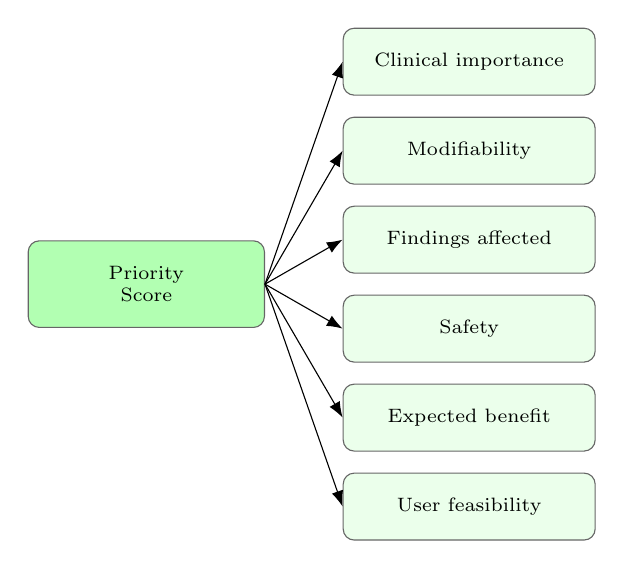
\begin{tikzpicture}[>=Latex]
\node[draw=black!60,rounded corners,fill=green!30,minimum width=3.0cm,minimum height=1.1cm,align=center,font=\scriptsize,text width=2.75cm,inner sep=2pt] (cc) at (0,-2.825) {Priority\\Score};
\node[draw=black!60,rounded corners,fill=green!8,minimum width=3.2cm,minimum height=0.85cm,align=center,font=\scriptsize,text width=2.95cm,inner sep=2pt] (sp0) at (4.1,0) {Clinical importance};
\draw[-{Latex[length=2mm]}] (cc.east)--(sp0.west);
\node[draw=black!60,rounded corners,fill=green!8,minimum width=3.2cm,minimum height=0.85cm,align=center,font=\scriptsize,text width=2.95cm,inner sep=2pt] (sp1) at (4.1,-1.13) {Modifiability};
\draw[-{Latex[length=2mm]}] (cc.east)--(sp1.west);
\node[draw=black!60,rounded corners,fill=green!8,minimum width=3.2cm,minimum height=0.85cm,align=center,font=\scriptsize,text width=2.95cm,inner sep=2pt] (sp2) at (4.1,-2.26) {Findings affected};
\draw[-{Latex[length=2mm]}] (cc.east)--(sp2.west);
\node[draw=black!60,rounded corners,fill=green!8,minimum width=3.2cm,minimum height=0.85cm,align=center,font=\scriptsize,text width=2.95cm,inner sep=2pt] (sp3) at (4.1,-3.3899999999999997) {Safety};
\draw[-{Latex[length=2mm]}] (cc.east)--(sp3.west);
\node[draw=black!60,rounded corners,fill=green!8,minimum width=3.2cm,minimum height=0.85cm,align=center,font=\scriptsize,text width=2.95cm,inner sep=2pt] (sp4) at (4.1,-4.52) {Expected benefit};
\draw[-{Latex[length=2mm]}] (cc.east)--(sp4.west);
\node[draw=black!60,rounded corners,fill=green!8,minimum width=3.2cm,minimum height=0.85cm,align=center,font=\scriptsize,text width=2.95cm,inner sep=2pt] (sp5) at (4.1,-5.6499999999999995) {User feasibility};
\draw[-{Latex[length=2mm]}] (cc.east)--(sp5.west);
\end{tikzpicture}
\end{adjustbox}
\end{center}
\end{frame}

\begin{frame}{Module 17: Recommendation Priority System}
\textcolor{black!55}{\scriptsize Schematic 2 -- Input / Output relations}\\[2pt]
\begin{center}
\begin{adjustbox}{max width=0.96\linewidth,max height=0.66\textheight}
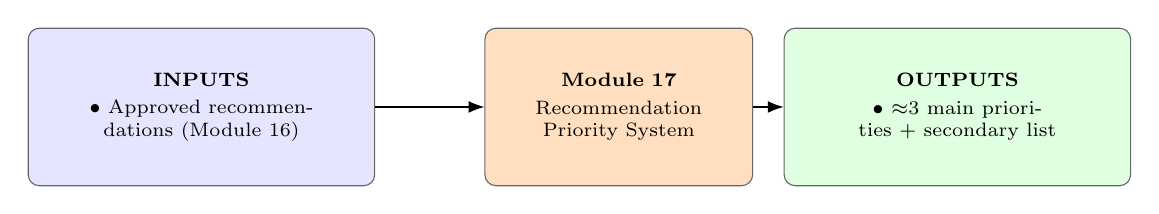
\begin{tikzpicture}[>=Latex]
\node[draw=black!60,rounded corners,fill=blue!10,minimum width=4.4cm,minimum height=2.0cm,align=center,font=\scriptsize,text width=4.15cm,inner sep=2pt] (io_in) at (0,0) {\textbf{\scriptsize INPUTS}\\[2pt]$\bullet$ Approved recommendations (Module 16)};
\node[draw=black!60,rounded corners,fill=orange!25,minimum width=3.4cm,minimum height=2.0cm,align=center,font=\scriptsize,text width=3.15cm,inner sep=2pt] (io_p) at (5.3,0) {\textbf{Module 17}\\[2pt]Recommendation Priority System};
\node[draw=black!60,rounded corners,fill=green!12,minimum width=4.4cm,minimum height=2.0cm,align=center,font=\scriptsize,text width=4.15cm,inner sep=2pt] (io_out) at (9.6,0) {\textbf{\scriptsize OUTPUTS}\\[2pt]$\bullet$ $\approx$3 main priorities + secondary list};
\draw[-{Latex[length=2mm]}] (io_in.east)--(io_p.west);
\draw[-{Latex[length=2mm]}] (io_p.east)--(io_out.west);
\end{tikzpicture}
\end{adjustbox}
\end{center}
\end{frame}

\begin{frame}{Module 18: Explanation Engine}
\textcolor{black!55}{\scriptsize Cluster 6 -- \textcolor{green!60!black}{\textbf{Recommendation \& Explanation}} (M15--M18)}\\[2pt]
\begin{columns}[T,onlytextwidth]
\begin{column}{0.5\textwidth}
\begin{tcolorbox}[colback=blue!7,colframe=blue!55!black,title=\textbf{Motivation},boxrule=0.6pt,arc=1mm,left=5pt,right=5pt,top=3pt,bottom=3pt,fonttitle=\small]
\footnotesize A recommendation without reasoning invites distrust and non-adherence.
\end{tcolorbox}
\vspace{5pt}
\begin{tcolorbox}[colback=teal!7,colframe=teal!55!black,title=\textbf{Method},boxrule=0.6pt,arc=1mm,left=5pt,right=5pt,top=3pt,bottom=3pt,fonttitle=\small]
\footnotesize Attach six structured fields to every recommendation, from what was found to what happens next.
\end{tcolorbox}
\end{column}
\begin{column}{0.5\textwidth}
\begin{tcolorbox}[colback=green!8,colframe=green!45!black,title=\textbf{Result},boxrule=0.6pt,arc=1mm,left=5pt,right=5pt,top=3pt,bottom=3pt,fonttitle=\small]
\footnotesize A fully reasoned explanation the user can read start-to-finish.
\end{tcolorbox}
\vspace{5pt}
\begin{tcolorbox}[colback=orange!10,colframe=orange!65!black,title=\textbf{Conclusion},boxrule=0.6pt,arc=1mm,left=5pt,right=5pt,top=3pt,bottom=3pt,fonttitle=\small]
\footnotesize Explaining the \textquotedblleft why\textquotedblright\ is what makes the platform feel like guidance, not a black box.
\end{tcolorbox}
\end{column}
\end{columns}
\end{frame}

\begin{frame}{Module 18: Explanation Engine}
\textcolor{black!55}{\scriptsize Schematic 1 -- Six-step explanation sequence}\\[2pt]
\begin{center}
\begin{adjustbox}{max width=0.96\linewidth,max height=0.66\textheight}
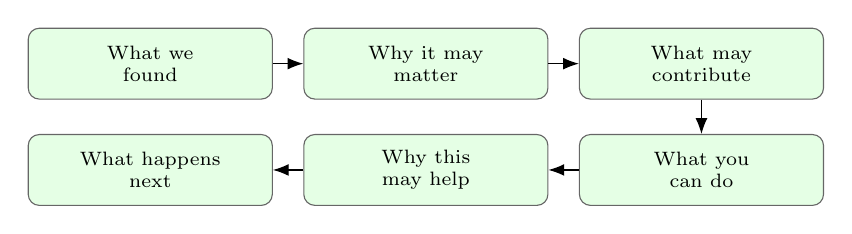
\begin{tikzpicture}[>=Latex]
\node[draw=black!60,rounded corners,fill=green!10,minimum width=3.1cm,minimum height=0.9cm,align=center,font=\scriptsize,text width=2.85cm,inner sep=2pt] (s0) at (0.0,0.0) {What we\\found};
\node[draw=black!60,rounded corners,fill=green!10,minimum width=3.1cm,minimum height=0.9cm,align=center,font=\scriptsize,text width=2.85cm,inner sep=2pt] (s1) at (3.5,0.0) {Why it may\\matter};
\node[draw=black!60,rounded corners,fill=green!10,minimum width=3.1cm,minimum height=0.9cm,align=center,font=\scriptsize,text width=2.85cm,inner sep=2pt] (s2) at (7.0,0.0) {What may\\contribute};
\node[draw=black!60,rounded corners,fill=green!10,minimum width=3.1cm,minimum height=0.9cm,align=center,font=\scriptsize,text width=2.85cm,inner sep=2pt] (s3) at (7.0,-1.35) {What you\\can do};
\node[draw=black!60,rounded corners,fill=green!10,minimum width=3.1cm,minimum height=0.9cm,align=center,font=\scriptsize,text width=2.85cm,inner sep=2pt] (s4) at (3.5,-1.35) {Why this\\may help};
\node[draw=black!60,rounded corners,fill=green!10,minimum width=3.1cm,minimum height=0.9cm,align=center,font=\scriptsize,text width=2.85cm,inner sep=2pt] (s5) at (0.0,-1.35) {What happens\\next};
\draw[-{Latex[length=2mm]}] (s0.east)--(s1.west);
\draw[-{Latex[length=2mm]}] (s1.east)--(s2.west);
\draw[-{Latex[length=2mm]}] (s2.south)--(s3.north);
\draw[-{Latex[length=2mm]}] (s3.west)--(s4.east);
\draw[-{Latex[length=2mm]}] (s4.west)--(s5.east);
\end{tikzpicture}
\end{adjustbox}
\end{center}
\end{frame}

\begin{frame}{Module 18: Explanation Engine}
\textcolor{black!55}{\scriptsize Schematic 2 -- Input / Output relations}\\[2pt]
\begin{center}
\begin{adjustbox}{max width=0.96\linewidth,max height=0.66\textheight}
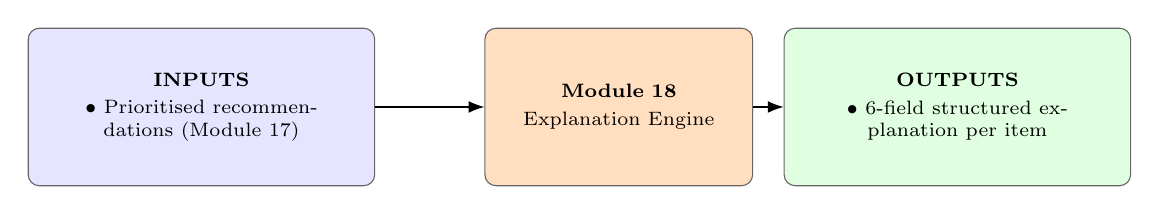
\begin{tikzpicture}[>=Latex]
\node[draw=black!60,rounded corners,fill=blue!10,minimum width=4.4cm,minimum height=2.0cm,align=center,font=\scriptsize,text width=4.15cm,inner sep=2pt] (io_in) at (0,0) {\textbf{\scriptsize INPUTS}\\[2pt]$\bullet$ Prioritised recommendations (Module 17)};
\node[draw=black!60,rounded corners,fill=orange!25,minimum width=3.4cm,minimum height=2.0cm,align=center,font=\scriptsize,text width=3.15cm,inner sep=2pt] (io_p) at (5.3,0) {\textbf{Module 18}\\[2pt]Explanation Engine};
\node[draw=black!60,rounded corners,fill=green!12,minimum width=4.4cm,minimum height=2.0cm,align=center,font=\scriptsize,text width=4.15cm,inner sep=2pt] (io_out) at (9.6,0) {\textbf{\scriptsize OUTPUTS}\\[2pt]$\bullet$ 6-field structured explanation per item};
\draw[-{Latex[length=2mm]}] (io_in.east)--(io_p.west);
\draw[-{Latex[length=2mm]}] (io_p.east)--(io_out.west);
\end{tikzpicture}
\end{adjustbox}
\end{center}
\end{frame}

\section{Cluster 7 -- Reporting \& Tracking (M19--M20)}

\begin{frame}{Module 19: Final User Report}
\textcolor{black!55}{\scriptsize Cluster 7 -- \textcolor{brown}{\textbf{Reporting \& Tracking}} (M19--M20)}\\[2pt]
\begin{columns}[T,onlytextwidth]
\begin{column}{0.5\textwidth}
\begin{tcolorbox}[colback=blue!7,colframe=blue!55!black,title=\textbf{Motivation},boxrule=0.6pt,arc=1mm,left=5pt,right=5pt,top=3pt,bottom=3pt,fonttitle=\small]
\footnotesize Findings, patterns and recommendations need one coherent document, not scattered outputs.
\end{tcolorbox}
\vspace{5pt}
\begin{tcolorbox}[colback=teal!7,colframe=teal!55!black,title=\textbf{Method},boxrule=0.6pt,arc=1mm,left=5pt,right=5pt,top=3pt,bottom=3pt,fonttitle=\small]
\footnotesize Assemble eight fixed sections, from Health Snapshot through Monitoring Plan, in a consistent order.
\end{tcolorbox}
\end{column}
\begin{column}{0.5\textwidth}
\begin{tcolorbox}[colback=green!8,colframe=green!45!black,title=\textbf{Result},boxrule=0.6pt,arc=1mm,left=5pt,right=5pt,top=3pt,bottom=3pt,fonttitle=\small]
\footnotesize A single, navigable report the user receives after every analysis.
\end{tcolorbox}
\vspace{5pt}
\begin{tcolorbox}[colback=orange!10,colframe=orange!65!black,title=\textbf{Conclusion},boxrule=0.6pt,arc=1mm,left=5pt,right=5pt,top=3pt,bottom=3pt,fonttitle=\small]
\footnotesize Consistent structure is what makes repeat reports comparable over time.
\end{tcolorbox}
\end{column}
\end{columns}
\end{frame}

\begin{frame}{Module 19: Final User Report}
\textcolor{black!55}{\scriptsize Schematic 1 -- Eight sections, fixed reading order}\\[2pt]
\begin{center}
\begin{adjustbox}{max width=0.96\linewidth,max height=0.66\textheight}
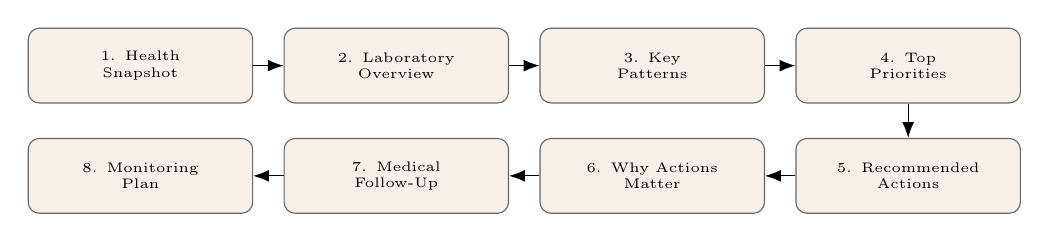
\begin{tikzpicture}[>=Latex]
\node[draw=black!60,rounded corners,fill=brown!12,minimum width=2.85cm,minimum height=0.95cm,align=center,font=\tiny,text width=2.6cm,inner sep=2pt] (s0) at (0.0,0.0) {1. Health\\Snapshot};
\node[draw=black!60,rounded corners,fill=brown!12,minimum width=2.85cm,minimum height=0.95cm,align=center,font=\tiny,text width=2.6cm,inner sep=2pt] (s1) at (3.25,0.0) {2. Laboratory\\Overview};
\node[draw=black!60,rounded corners,fill=brown!12,minimum width=2.85cm,minimum height=0.95cm,align=center,font=\tiny,text width=2.6cm,inner sep=2pt] (s2) at (6.5,0.0) {3. Key\\Patterns};
\node[draw=black!60,rounded corners,fill=brown!12,minimum width=2.85cm,minimum height=0.95cm,align=center,font=\tiny,text width=2.6cm,inner sep=2pt] (s3) at (9.75,0.0) {4. Top\\Priorities};
\node[draw=black!60,rounded corners,fill=brown!12,minimum width=2.85cm,minimum height=0.95cm,align=center,font=\tiny,text width=2.6cm,inner sep=2pt] (s4) at (9.75,-1.4) {5. Recommended\\Actions};
\node[draw=black!60,rounded corners,fill=brown!12,minimum width=2.85cm,minimum height=0.95cm,align=center,font=\tiny,text width=2.6cm,inner sep=2pt] (s5) at (6.5,-1.4) {6. Why Actions\\Matter};
\node[draw=black!60,rounded corners,fill=brown!12,minimum width=2.85cm,minimum height=0.95cm,align=center,font=\tiny,text width=2.6cm,inner sep=2pt] (s6) at (3.25,-1.4) {7. Medical\\Follow-Up};
\node[draw=black!60,rounded corners,fill=brown!12,minimum width=2.85cm,minimum height=0.95cm,align=center,font=\tiny,text width=2.6cm,inner sep=2pt] (s7) at (0.0,-1.4) {8. Monitoring\\Plan};
\draw[-{Latex[length=2mm]}] (s0.east)--(s1.west);
\draw[-{Latex[length=2mm]}] (s1.east)--(s2.west);
\draw[-{Latex[length=2mm]}] (s2.east)--(s3.west);
\draw[-{Latex[length=2mm]}] (s3.south)--(s4.north);
\draw[-{Latex[length=2mm]}] (s4.west)--(s5.east);
\draw[-{Latex[length=2mm]}] (s5.west)--(s6.east);
\draw[-{Latex[length=2mm]}] (s6.west)--(s7.east);
\end{tikzpicture}
\end{adjustbox}
\end{center}
\end{frame}

\begin{frame}{Module 19: Final User Report}
\textcolor{black!55}{\scriptsize Schematic 2 -- Input / Output relations}\\[2pt]
\begin{center}
\begin{adjustbox}{max width=0.96\linewidth,max height=0.66\textheight}
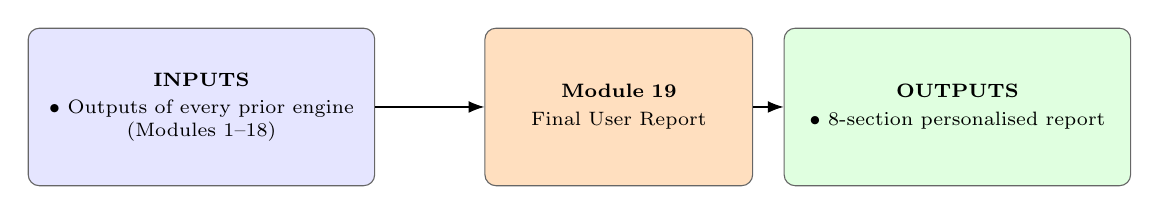
\begin{tikzpicture}[>=Latex]
\node[draw=black!60,rounded corners,fill=blue!10,minimum width=4.4cm,minimum height=2.0cm,align=center,font=\scriptsize,text width=4.15cm,inner sep=2pt] (io_in) at (0,0) {\textbf{\scriptsize INPUTS}\\[2pt]$\bullet$ Outputs of every prior engine\\(Modules 1--18)};
\node[draw=black!60,rounded corners,fill=orange!25,minimum width=3.4cm,minimum height=2.0cm,align=center,font=\scriptsize,text width=3.15cm,inner sep=2pt] (io_p) at (5.3,0) {\textbf{Module 19}\\[2pt]Final User Report};
\node[draw=black!60,rounded corners,fill=green!12,minimum width=4.4cm,minimum height=2.0cm,align=center,font=\scriptsize,text width=4.15cm,inner sep=2pt] (io_out) at (9.6,0) {\textbf{\scriptsize OUTPUTS}\\[2pt]$\bullet$ 8-section personalised report};
\draw[-{Latex[length=2mm]}] (io_in.east)--(io_p.west);
\draw[-{Latex[length=2mm]}] (io_p.east)--(io_out.west);
\end{tikzpicture}
\end{adjustbox}
\end{center}
\end{frame}

\begin{frame}{Module 20: Longitudinal Tracking}
\textcolor{black!55}{\scriptsize Cluster 7 -- \textcolor{brown}{\textbf{Reporting \& Tracking}} (M19--M20)}\\[2pt]
\begin{columns}[T,onlytextwidth]
\begin{column}{0.5\textwidth}
\begin{tcolorbox}[colback=blue!7,colframe=blue!55!black,title=\textbf{Motivation},boxrule=0.6pt,arc=1mm,left=5pt,right=5pt,top=3pt,bottom=3pt,fonttitle=\small]
\footnotesize A single time-point result cannot show whether a person's health is improving.
\end{tcolorbox}
\vspace{5pt}
\begin{tcolorbox}[colback=teal!7,colframe=teal!55!black,title=\textbf{Method},boxrule=0.6pt,arc=1mm,left=5pt,right=5pt,top=3pt,bottom=3pt,fonttitle=\small]
\footnotesize Store every result against its date and classify multi-point series into a trend category.
\end{tcolorbox}
\end{column}
\begin{column}{0.5\textwidth}
\begin{tcolorbox}[colback=green!8,colframe=green!45!black,title=\textbf{Result},boxrule=0.6pt,arc=1mm,left=5pt,right=5pt,top=3pt,bottom=3pt,fonttitle=\small]
\footnotesize Trend-aware statements (e.g. \textquotedblleft progressive upward trend across three measurements\textquotedblright) instead of isolated snapshots.
\end{tcolorbox}
\vspace{5pt}
\begin{tcolorbox}[colback=orange!10,colframe=orange!65!black,title=\textbf{Conclusion},boxrule=0.6pt,arc=1mm,left=5pt,right=5pt,top=3pt,bottom=3pt,fonttitle=\small]
\footnotesize Tracking is what turns MyHealthReport from a one-off reading into an ongoing health record.
\end{tcolorbox}
\end{column}
\end{columns}
\end{frame}

\begin{frame}{Module 20: Longitudinal Tracking}
\textcolor{black!55}{\scriptsize Schematic 1 -- A rising HbA1c series classified as Worsening}\\[2pt]
\begin{center}
\begin{adjustbox}{max width=0.96\linewidth,max height=0.66\textheight}
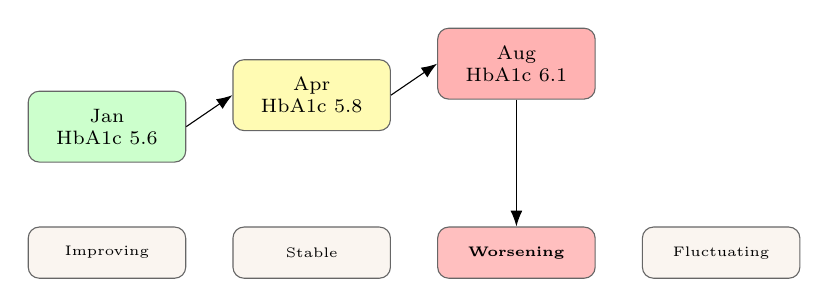
\begin{tikzpicture}[>=Latex]
\node[draw=black!60,rounded corners,fill=green!20,minimum width=2.0cm,minimum height=0.9cm,align=center,font=\scriptsize,text width=1.75cm,inner sep=2pt] (t1) at (0,0.2) {Jan\\HbA1c 5.6};
\node[draw=black!60,rounded corners,fill=yellow!30,minimum width=2.0cm,minimum height=0.9cm,align=center,font=\scriptsize,text width=1.75cm,inner sep=2pt] (t2) at (2.6,0.6) {Apr\\HbA1c 5.8};
\node[draw=black!60,rounded corners,fill=red!30,minimum width=2.0cm,minimum height=0.9cm,align=center,font=\scriptsize,text width=1.75cm,inner sep=2pt] (t3) at (5.2,1.0) {Aug\\HbA1c 6.1};
\draw[-{Latex[length=2mm]}] (t1.east)--(t2.west);
\draw[-{Latex[length=2mm]}] (t2.east)--(t3.west);
\node[draw=black!60,rounded corners,fill=brown!8,minimum width=2.0cm,minimum height=0.65cm,align=center,font=\tiny,text width=1.75cm,inner sep=2pt] (tc1) at (0,-1.4) {Improving};
\node[draw=black!60,rounded corners,fill=brown!8,minimum width=2.0cm,minimum height=0.65cm,align=center,font=\tiny,text width=1.75cm,inner sep=2pt] (tc2) at (2.6,-1.4) {Stable};
\node[draw=black!60,rounded corners,fill=red!25,minimum width=2.0cm,minimum height=0.65cm,align=center,font=\tiny,text width=1.75cm,inner sep=2pt] (tc3) at (5.2,-1.4) {\textbf{Worsening}};
\node[draw=black!60,rounded corners,fill=brown!8,minimum width=2.0cm,minimum height=0.65cm,align=center,font=\tiny,text width=1.75cm,inner sep=2pt] (tc4) at (7.8,-1.4) {Fluctuating};
\draw[-{Latex[length=2mm]}] (t3.south)--(tc3.north);
\end{tikzpicture}
\end{adjustbox}
\end{center}
\end{frame}

\begin{frame}{Module 20: Longitudinal Tracking}
\textcolor{black!55}{\scriptsize Schematic 2 -- Input / Output relations}\\[2pt]
\begin{center}
\begin{adjustbox}{max width=0.96\linewidth,max height=0.66\textheight}
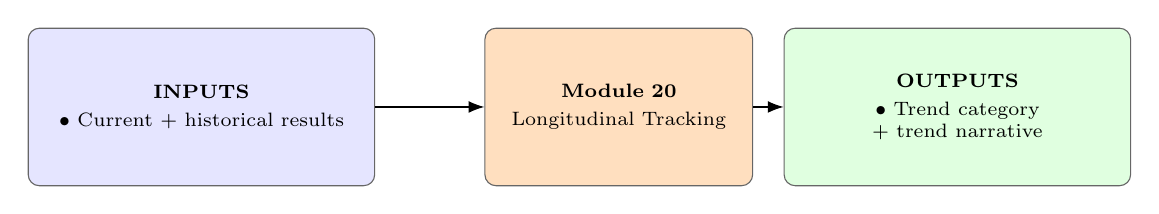
\begin{tikzpicture}[>=Latex]
\node[draw=black!60,rounded corners,fill=blue!10,minimum width=4.4cm,minimum height=2.0cm,align=center,font=\scriptsize,text width=4.15cm,inner sep=2pt] (io_in) at (0,0) {\textbf{\scriptsize INPUTS}\\[2pt]$\bullet$ Current + historical results};
\node[draw=black!60,rounded corners,fill=orange!25,minimum width=3.4cm,minimum height=2.0cm,align=center,font=\scriptsize,text width=3.15cm,inner sep=2pt] (io_p) at (5.3,0) {\textbf{Module 20}\\[2pt]Longitudinal Tracking};
\node[draw=black!60,rounded corners,fill=green!12,minimum width=4.4cm,minimum height=2.0cm,align=center,font=\scriptsize,text width=4.15cm,inner sep=2pt] (io_out) at (9.6,0) {\textbf{\scriptsize OUTPUTS}\\[2pt]$\bullet$ Trend category + trend narrative};
\draw[-{Latex[length=2mm]}] (io_in.east)--(io_p.west);
\draw[-{Latex[length=2mm]}] (io_p.east)--(io_out.west);
\end{tikzpicture}
\end{adjustbox}
\end{center}
\end{frame}

\section{Data, Rules \& AI Governance}

\begin{frame}{25. Version 1 Database Concept}
\begin{columns}[T,onlytextwidth]
\begin{column}{0.5\textwidth}
\begin{tcolorbox}[colback=blue!7,colframe=blue!55!black,title=\textbf{Motivation},boxrule=0.6pt,arc=1mm,left=5pt,right=5pt,top=3pt,bottom=3pt,fonttitle=\small]
\footnotesize Free-text storage cannot support rules, triggers, or trend analysis.
\end{tcolorbox}
\vspace{5pt}
\begin{tcolorbox}[colback=teal!7,colframe=teal!55!black,title=\textbf{Method},boxrule=0.6pt,arc=1mm,left=5pt,right=5pt,top=3pt,bottom=3pt,fonttitle=\small]
\footnotesize Define 13 core structured objects covering patient data, findings, rules and recommendations.
\end{tcolorbox}
\end{column}
\begin{column}{0.5\textwidth}
\begin{tcolorbox}[colback=green!8,colframe=green!45!black,title=\textbf{Result},boxrule=0.6pt,arc=1mm,left=5pt,right=5pt,top=3pt,bottom=3pt,fonttitle=\small]
\footnotesize A relational data model underlying every module in the pipeline.
\end{tcolorbox}
\vspace{5pt}
\begin{tcolorbox}[colback=orange!10,colframe=orange!65!black,title=\textbf{Conclusion},boxrule=0.6pt,arc=1mm,left=5pt,right=5pt,top=3pt,bottom=3pt,fonttitle=\small]
\footnotesize Every module in this deck reads or writes one or more of these 13 objects.
\end{tcolorbox}
\end{column}
\end{columns}
\end{frame}

\begin{frame}{25. Version 1 Database Concept}
\textcolor{black!55}{\scriptsize Thirteen core structured objects}\\[2pt]
\begin{center}
\begin{adjustbox}{max width=0.96\linewidth,max height=0.66\textheight}
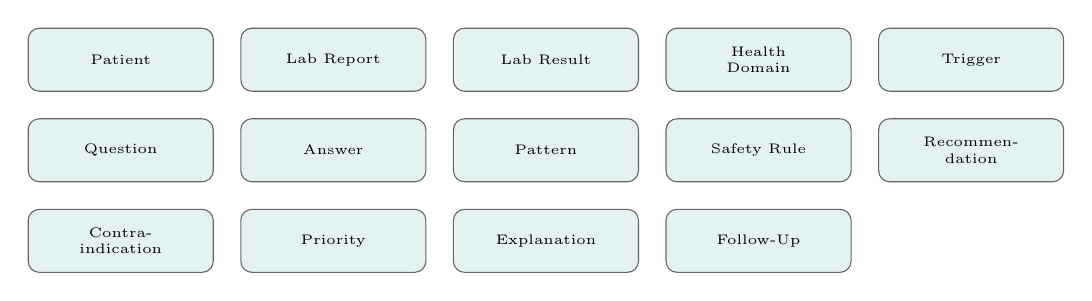
\begin{tikzpicture}[>=Latex]
\node[draw=black!60,rounded corners,fill=teal!10,minimum width=2.35cm,minimum height=0.8cm,align=center,font=\tiny,text width=2.1cm,inner sep=2pt] (g0) at (0.0,0.0) {Patient};
\node[draw=black!60,rounded corners,fill=teal!10,minimum width=2.35cm,minimum height=0.8cm,align=center,font=\tiny,text width=2.1cm,inner sep=2pt] (g1) at (2.7,0.0) {Lab Report};
\node[draw=black!60,rounded corners,fill=teal!10,minimum width=2.35cm,minimum height=0.8cm,align=center,font=\tiny,text width=2.1cm,inner sep=2pt] (g2) at (5.4,0.0) {Lab Result};
\node[draw=black!60,rounded corners,fill=teal!10,minimum width=2.35cm,minimum height=0.8cm,align=center,font=\tiny,text width=2.1cm,inner sep=2pt] (g3) at (8.100000000000001,0.0) {Health\\Domain};
\node[draw=black!60,rounded corners,fill=teal!10,minimum width=2.35cm,minimum height=0.8cm,align=center,font=\tiny,text width=2.1cm,inner sep=2pt] (g4) at (10.8,0.0) {Trigger};
\node[draw=black!60,rounded corners,fill=teal!10,minimum width=2.35cm,minimum height=0.8cm,align=center,font=\tiny,text width=2.1cm,inner sep=2pt] (g5) at (0.0,-1.15) {Question};
\node[draw=black!60,rounded corners,fill=teal!10,minimum width=2.35cm,minimum height=0.8cm,align=center,font=\tiny,text width=2.1cm,inner sep=2pt] (g6) at (2.7,-1.15) {Answer};
\node[draw=black!60,rounded corners,fill=teal!10,minimum width=2.35cm,minimum height=0.8cm,align=center,font=\tiny,text width=2.1cm,inner sep=2pt] (g7) at (5.4,-1.15) {Pattern};
\node[draw=black!60,rounded corners,fill=teal!10,minimum width=2.35cm,minimum height=0.8cm,align=center,font=\tiny,text width=2.1cm,inner sep=2pt] (g8) at (8.100000000000001,-1.15) {Safety Rule};
\node[draw=black!60,rounded corners,fill=teal!10,minimum width=2.35cm,minimum height=0.8cm,align=center,font=\tiny,text width=2.1cm,inner sep=2pt] (g9) at (10.8,-1.15) {Recommen-\\dation};
\node[draw=black!60,rounded corners,fill=teal!10,minimum width=2.35cm,minimum height=0.8cm,align=center,font=\tiny,text width=2.1cm,inner sep=2pt] (g10) at (0.0,-2.3) {Contra-\\indication};
\node[draw=black!60,rounded corners,fill=teal!10,minimum width=2.35cm,minimum height=0.8cm,align=center,font=\tiny,text width=2.1cm,inner sep=2pt] (g11) at (2.7,-2.3) {Priority};
\node[draw=black!60,rounded corners,fill=teal!10,minimum width=2.35cm,minimum height=0.8cm,align=center,font=\tiny,text width=2.1cm,inner sep=2pt] (g12) at (5.4,-2.3) {Explanation};
\node[draw=black!60,rounded corners,fill=teal!10,minimum width=2.35cm,minimum height=0.8cm,align=center,font=\tiny,text width=2.1cm,inner sep=2pt] (g13) at (8.100000000000001,-2.3) {Follow-Up};
\end{tikzpicture}
\end{adjustbox}
\end{center}
\end{frame}

\begin{frame}{26. Master Rule Architecture}
\begin{columns}[T,onlytextwidth]
\begin{column}{0.5\textwidth}
\begin{tcolorbox}[colback=blue!7,colframe=blue!55!black,title=\textbf{Motivation},boxrule=0.6pt,arc=1mm,left=5pt,right=5pt,top=3pt,bottom=3pt,fonttitle=\small]
\footnotesize Twenty modules need one shared rule shape, or the logic becomes unmaintainable.
\end{tcolorbox}
\vspace{5pt}
\begin{tcolorbox}[colback=teal!7,colframe=teal!55!black,title=\textbf{Method},boxrule=0.6pt,arc=1mm,left=5pt,right=5pt,top=3pt,bottom=3pt,fonttitle=\small]
\footnotesize Express every clinical/wellness rule as: IF Finding + Context THEN Question $\to$ Safety $\to$ Pattern $\to$ Recommendation UNLESS Contraindication THEN Priority + Explanation + Follow-Up.
\end{tcolorbox}
\end{column}
\begin{column}{0.5\textwidth}
\begin{tcolorbox}[colback=green!8,colframe=green!45!black,title=\textbf{Result},boxrule=0.6pt,arc=1mm,left=5pt,right=5pt,top=3pt,bottom=3pt,fonttitle=\small]
\footnotesize A single reusable rule template applied across all 20 modules.
\end{tcolorbox}
\vspace{5pt}
\begin{tcolorbox}[colback=orange!10,colframe=orange!65!black,title=\textbf{Conclusion},boxrule=0.6pt,arc=1mm,left=5pt,right=5pt,top=3pt,bottom=3pt,fonttitle=\small]
\footnotesize This is the syntax the Four Master Matrices (Topic 31) are written in.
\end{tcolorbox}
\end{column}
\end{columns}
\end{frame}

\begin{frame}{26. Master Rule Architecture}
\textcolor{black!55}{\scriptsize The IF...THEN...UNLESS rule template as a flow}\\[2pt]
\begin{center}
\begin{adjustbox}{max width=0.96\linewidth,max height=0.66\textheight}
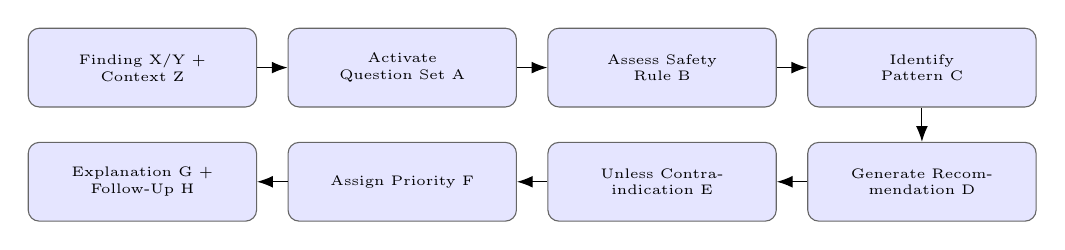
\begin{tikzpicture}[>=Latex]
\node[draw=black!60,rounded corners,fill=blue!10,minimum width=2.9cm,minimum height=1.0cm,align=center,font=\tiny,text width=2.65cm,inner sep=2pt] (s0) at (0.0,0.0) {Finding X/Y +\\Context Z};
\node[draw=black!60,rounded corners,fill=blue!10,minimum width=2.9cm,minimum height=1.0cm,align=center,font=\tiny,text width=2.65cm,inner sep=2pt] (s1) at (3.3,0.0) {Activate\\Question Set A};
\node[draw=black!60,rounded corners,fill=blue!10,minimum width=2.9cm,minimum height=1.0cm,align=center,font=\tiny,text width=2.65cm,inner sep=2pt] (s2) at (6.6,0.0) {Assess Safety\\Rule B};
\node[draw=black!60,rounded corners,fill=blue!10,minimum width=2.9cm,minimum height=1.0cm,align=center,font=\tiny,text width=2.65cm,inner sep=2pt] (s3) at (9.899999999999999,0.0) {Identify\\Pattern C};
\node[draw=black!60,rounded corners,fill=blue!10,minimum width=2.9cm,minimum height=1.0cm,align=center,font=\tiny,text width=2.65cm,inner sep=2pt] (s4) at (9.899999999999999,-1.45) {Generate Recom-\\mendation D};
\node[draw=black!60,rounded corners,fill=blue!10,minimum width=2.9cm,minimum height=1.0cm,align=center,font=\tiny,text width=2.65cm,inner sep=2pt] (s5) at (6.6,-1.45) {Unless Contra-\\indication E};
\node[draw=black!60,rounded corners,fill=blue!10,minimum width=2.9cm,minimum height=1.0cm,align=center,font=\tiny,text width=2.65cm,inner sep=2pt] (s6) at (3.3,-1.45) {Assign Priority F};
\node[draw=black!60,rounded corners,fill=blue!10,minimum width=2.9cm,minimum height=1.0cm,align=center,font=\tiny,text width=2.65cm,inner sep=2pt] (s7) at (0.0,-1.45) {Explanation G +\\Follow-Up H};
\draw[-{Latex[length=2mm]}] (s0.east)--(s1.west);
\draw[-{Latex[length=2mm]}] (s1.east)--(s2.west);
\draw[-{Latex[length=2mm]}] (s2.east)--(s3.west);
\draw[-{Latex[length=2mm]}] (s3.south)--(s4.north);
\draw[-{Latex[length=2mm]}] (s4.west)--(s5.east);
\draw[-{Latex[length=2mm]}] (s5.west)--(s6.east);
\draw[-{Latex[length=2mm]}] (s6.west)--(s7.east);
\end{tikzpicture}
\end{adjustbox}
\end{center}
\end{frame}

\begin{frame}{27. What AI Should Do}
\begin{columns}[T,onlytextwidth]
\begin{column}{0.5\textwidth}
\begin{tcolorbox}[colback=blue!7,colframe=blue!55!black,title=\textbf{Motivation},boxrule=0.6pt,arc=1mm,left=5pt,right=5pt,top=3pt,bottom=3pt,fonttitle=\small]
\footnotesize AI is capable of more than the platform should let it decide unsupervised.
\end{tcolorbox}
\vspace{5pt}
\begin{tcolorbox}[colback=teal!7,colframe=teal!55!black,title=\textbf{Method},boxrule=0.6pt,arc=1mm,left=5pt,right=5pt,top=3pt,bottom=3pt,fonttitle=\small]
\footnotesize Scope AI to extraction assistance, explanation, summarisation, wording, rule identification and report generation.
\end{tcolorbox}
\end{column}
\begin{column}{0.5\textwidth}
\begin{tcolorbox}[colback=green!8,colframe=green!45!black,title=\textbf{Result},boxrule=0.6pt,arc=1mm,left=5pt,right=5pt,top=3pt,bottom=3pt,fonttitle=\small]
\footnotesize A bounded, non-clinical role for AI within the pipeline.
\end{tcolorbox}
\vspace{5pt}
\begin{tcolorbox}[colback=orange!10,colframe=orange!65!black,title=\textbf{Conclusion},boxrule=0.6pt,arc=1mm,left=5pt,right=5pt,top=3pt,bottom=3pt,fonttitle=\small]
\footnotesize AI accelerates communication; it does not originate clinical judgment.
\end{tcolorbox}
\end{column}
\end{columns}
\end{frame}

\begin{frame}{27. What AI Should Do}
\textcolor{black!55}{\scriptsize Six permitted AI functions, radiating from one bounded role}\\[2pt]
\begin{center}
\begin{adjustbox}{max width=0.96\linewidth,max height=0.66\textheight}
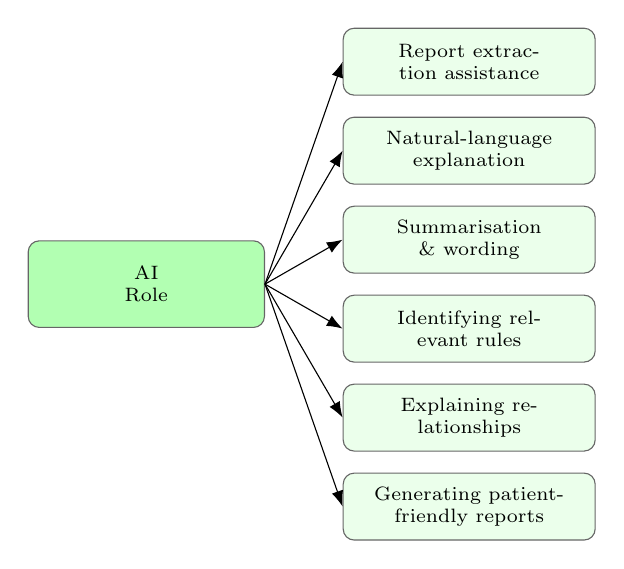
\begin{tikzpicture}[>=Latex]
\node[draw=black!60,rounded corners,fill=green!30,minimum width=3.0cm,minimum height=1.1cm,align=center,font=\scriptsize,text width=2.75cm,inner sep=2pt] (cc) at (0,-2.825) {AI\\Role};
\node[draw=black!60,rounded corners,fill=green!8,minimum width=3.2cm,minimum height=0.85cm,align=center,font=\scriptsize,text width=2.95cm,inner sep=2pt] (sp0) at (4.1,0) {Report extraction assistance};
\draw[-{Latex[length=2mm]}] (cc.east)--(sp0.west);
\node[draw=black!60,rounded corners,fill=green!8,minimum width=3.2cm,minimum height=0.85cm,align=center,font=\scriptsize,text width=2.95cm,inner sep=2pt] (sp1) at (4.1,-1.13) {Natural-language explanation};
\draw[-{Latex[length=2mm]}] (cc.east)--(sp1.west);
\node[draw=black!60,rounded corners,fill=green!8,minimum width=3.2cm,minimum height=0.85cm,align=center,font=\scriptsize,text width=2.95cm,inner sep=2pt] (sp2) at (4.1,-2.26) {Summarisation \& wording};
\draw[-{Latex[length=2mm]}] (cc.east)--(sp2.west);
\node[draw=black!60,rounded corners,fill=green!8,minimum width=3.2cm,minimum height=0.85cm,align=center,font=\scriptsize,text width=2.95cm,inner sep=2pt] (sp3) at (4.1,-3.3899999999999997) {Identifying relevant rules};
\draw[-{Latex[length=2mm]}] (cc.east)--(sp3.west);
\node[draw=black!60,rounded corners,fill=green!8,minimum width=3.2cm,minimum height=0.85cm,align=center,font=\scriptsize,text width=2.95cm,inner sep=2pt] (sp4) at (4.1,-4.52) {Explaining relationships};
\draw[-{Latex[length=2mm]}] (cc.east)--(sp4.west);
\node[draw=black!60,rounded corners,fill=green!8,minimum width=3.2cm,minimum height=0.85cm,align=center,font=\scriptsize,text width=2.95cm,inner sep=2pt] (sp5) at (4.1,-5.6499999999999995) {Generating patient-friendly reports};
\draw[-{Latex[length=2mm]}] (cc.east)--(sp5.west);
\end{tikzpicture}
\end{adjustbox}
\end{center}
\end{frame}

\begin{frame}{28. What AI Should NOT Independently Control}
\begin{columns}[T,onlytextwidth]
\begin{column}{0.5\textwidth}
\begin{tcolorbox}[colback=blue!7,colframe=blue!55!black,title=\textbf{Motivation},boxrule=0.6pt,arc=1mm,left=5pt,right=5pt,top=3pt,bottom=3pt,fonttitle=\small]
\footnotesize Letting AI freely decide safety-critical logic risks an unvalidated claim reaching a user.
\end{tcolorbox}
\vspace{5pt}
\begin{tcolorbox}[colback=teal!7,colframe=teal!55!black,title=\textbf{Method},boxrule=0.6pt,arc=1mm,left=5pt,right=5pt,top=3pt,bottom=3pt,fonttitle=\small]
\footnotesize Reserve emergency triggers, thresholds, contraindications, referral criteria, diagnosis and medication advice to rule-governed logic only.
\end{tcolorbox}
\end{column}
\begin{column}{0.5\textwidth}
\begin{tcolorbox}[colback=green!8,colframe=green!45!black,title=\textbf{Result},boxrule=0.6pt,arc=1mm,left=5pt,right=5pt,top=3pt,bottom=3pt,fonttitle=\small]
\footnotesize A hard boundary between \textquotedblleft rules decide\textquotedblright\ and \textquotedblleft AI explains\textquotedblright.
\end{tcolorbox}
\vspace{5pt}
\begin{tcolorbox}[colback=orange!10,colframe=orange!65!black,title=\textbf{Conclusion},boxrule=0.6pt,arc=1mm,left=5pt,right=5pt,top=3pt,bottom=3pt,fonttitle=\small]
\footnotesize Structured clinical rules determine what is allowed; AI determines how it is explained.
\end{tcolorbox}
\end{column}
\end{columns}
\end{frame}

\begin{frame}{28. What AI Should NOT Independently Control}
\textcolor{black!55}{\scriptsize Six safety-critical elements, reserved to rule-governed logic}\\[2pt]
\begin{center}
\begin{adjustbox}{max width=0.96\linewidth,max height=0.66\textheight}
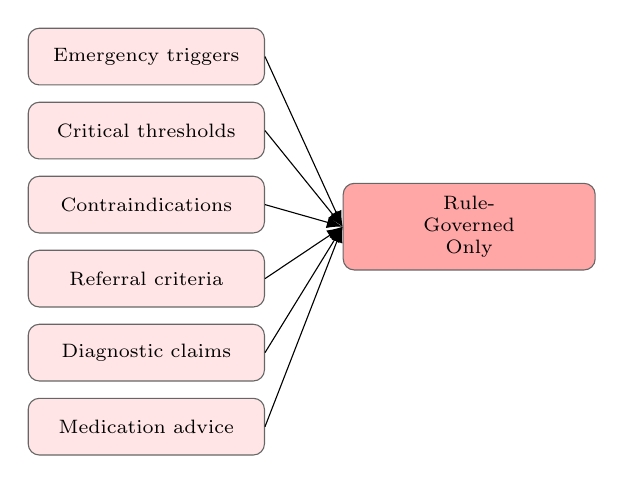
\begin{tikzpicture}[>=Latex]
\node[draw=black!60,rounded corners,fill=red!10,minimum width=3.0cm,minimum height=0.72cm,align=center,font=\scriptsize,text width=2.75cm,inner sep=2pt] (in0) at (0,0) {Emergency triggers};
\node[draw=black!60,rounded corners,fill=red!10,minimum width=3.0cm,minimum height=0.72cm,align=center,font=\scriptsize,text width=2.75cm,inner sep=2pt] (in1) at (0,-0.94) {Critical thresholds};
\node[draw=black!60,rounded corners,fill=red!10,minimum width=3.0cm,minimum height=0.72cm,align=center,font=\scriptsize,text width=2.75cm,inner sep=2pt] (in2) at (0,-1.88) {Contraindications};
\node[draw=black!60,rounded corners,fill=red!10,minimum width=3.0cm,minimum height=0.72cm,align=center,font=\scriptsize,text width=2.75cm,inner sep=2pt] (in3) at (0,-2.82) {Referral criteria};
\node[draw=black!60,rounded corners,fill=red!10,minimum width=3.0cm,minimum height=0.72cm,align=center,font=\scriptsize,text width=2.75cm,inner sep=2pt] (in4) at (0,-3.76) {Diagnostic claims};
\node[draw=black!60,rounded corners,fill=red!10,minimum width=3.0cm,minimum height=0.72cm,align=center,font=\scriptsize,text width=2.75cm,inner sep=2pt] (in5) at (0,-4.699999999999999) {Medication advice};
\node[draw=black!60,rounded corners,fill=red!35,minimum width=3.2cm,minimum height=1.1cm,align=center,font=\scriptsize,text width=2.95cm,inner sep=2pt] (cc2) at (4.1,-2.16) {Rule-\\Governed\\Only};
\draw[-{Latex[length=2mm]}] (in0.east)--(cc2.west);
\draw[-{Latex[length=2mm]}] (in1.east)--(cc2.west);
\draw[-{Latex[length=2mm]}] (in2.east)--(cc2.west);
\draw[-{Latex[length=2mm]}] (in3.east)--(cc2.west);
\draw[-{Latex[length=2mm]}] (in4.east)--(cc2.west);
\draw[-{Latex[length=2mm]}] (in5.east)--(cc2.west);
\end{tikzpicture}
\end{adjustbox}
\end{center}
\end{frame}

\section{Scope, Roadmap \& Matrices}

\begin{frame}{29. Version 1 Scope Boundary}
\begin{columns}[T,onlytextwidth]
\begin{column}{0.5\textwidth}
\begin{tcolorbox}[colback=blue!7,colframe=blue!55!black,title=\textbf{Motivation},boxrule=0.6pt,arc=1mm,left=5pt,right=5pt,top=3pt,bottom=3pt,fonttitle=\small]
\footnotesize An unbounded roadmap delays shipping a safe, useful Version 1.
\end{tcolorbox}
\vspace{5pt}
\begin{tcolorbox}[colback=teal!7,colframe=teal!55!black,title=\textbf{Method},boxrule=0.6pt,arc=1mm,left=5pt,right=5pt,top=3pt,bottom=3pt,fonttitle=\small]
\footnotesize Explicitly separate what Version 1 includes from what is delayed.
\end{tcolorbox}
\end{column}
\begin{column}{0.5\textwidth}
\begin{tcolorbox}[colback=green!8,colframe=green!45!black,title=\textbf{Result},boxrule=0.6pt,arc=1mm,left=5pt,right=5pt,top=3pt,bottom=3pt,fonttitle=\small]
\footnotesize A concrete in/out list reviewable against every new feature request.
\end{tcolorbox}
\vspace{5pt}
\begin{tcolorbox}[colback=orange!10,colframe=orange!65!black,title=\textbf{Conclusion},boxrule=0.6pt,arc=1mm,left=5pt,right=5pt,top=3pt,bottom=3pt,fonttitle=\small]
\footnotesize Saying no to Phase-2+ features is what keeps Version 1 shippable and safe.
\end{tcolorbox}
\end{column}
\end{columns}
\end{frame}

\begin{frame}{29. Version 1 Scope Boundary}
\textcolor{black!55}{\scriptsize Include vs. delay -- a reviewable boundary}\\[2pt]
\begin{center}
\begin{adjustbox}{max width=0.96\linewidth,max height=0.66\textheight}
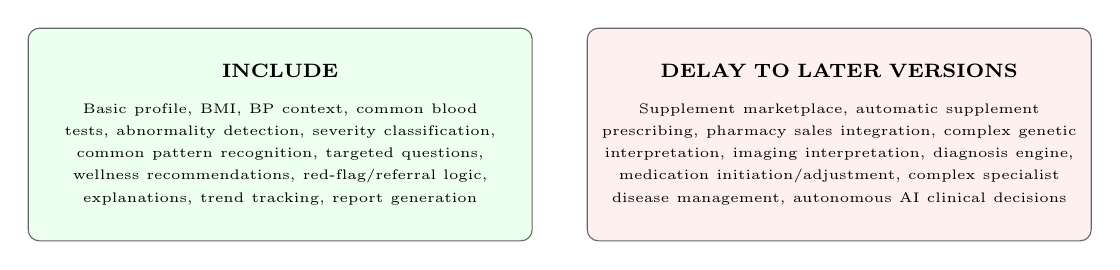
\begin{tikzpicture}[>=Latex]
\node[draw=black!60,rounded corners,fill=green!7,minimum width=6.4cm,minimum height=2.7cm,align=center,font=\scriptsize,text width=6.15cm,inner sep=2pt] (sc_inc) at (0,0) {\textbf{\scriptsize INCLUDE}\\[5pt]\tiny Basic profile, BMI, BP context, common blood tests, abnormality detection, severity classification, common pattern recognition, targeted questions, wellness recommendations, red-flag/referral logic, explanations, trend tracking, report generation};
\node[draw=black!60,rounded corners,fill=red!6,minimum width=6.4cm,minimum height=2.7cm,align=center,font=\scriptsize,text width=6.15cm,inner sep=2pt] (sc_del) at (7.1,0) {\textbf{\scriptsize DELAY TO LATER VERSIONS}\\[5pt]\tiny Supplement marketplace, automatic supplement prescribing, pharmacy sales integration, complex genetic interpretation, imaging interpretation, diagnosis engine, medication initiation/adjustment, complex specialist disease management, autonomous AI clinical decisions};
\end{tikzpicture}
\end{adjustbox}
\end{center}
\end{frame}

\begin{frame}{30. Clinical Domains to Build First}
\begin{columns}[T,onlytextwidth]
\begin{column}{0.5\textwidth}
\begin{tcolorbox}[colback=blue!7,colframe=blue!55!black,title=\textbf{Motivation},boxrule=0.6pt,arc=1mm,left=5pt,right=5pt,top=3pt,bottom=3pt,fonttitle=\small]
\footnotesize Building all eight lab domains simultaneously multiplies validation risk before any value ships.
\end{tcolorbox}
\vspace{5pt}
\begin{tcolorbox}[colback=teal!7,colframe=teal!55!black,title=\textbf{Method},boxrule=0.6pt,arc=1mm,left=5pt,right=5pt,top=3pt,bottom=3pt,fonttitle=\small]
\footnotesize Sequence domains by preventive-health impact across four build phases.
\end{tcolorbox}
\end{column}
\begin{column}{0.5\textwidth}
\begin{tcolorbox}[colback=green!8,colframe=green!45!black,title=\textbf{Result},boxrule=0.6pt,arc=1mm,left=5pt,right=5pt,top=3pt,bottom=3pt,fonttitle=\small]
\footnotesize A four-phase build order, not a simultaneous eight-domain launch.
\end{tcolorbox}
\vspace{5pt}
\begin{tcolorbox}[colback=orange!10,colframe=orange!65!black,title=\textbf{Conclusion},boxrule=0.6pt,arc=1mm,left=5pt,right=5pt,top=3pt,bottom=3pt,fonttitle=\small]
\footnotesize Depth-first on one domain beats shallow coverage of eight.
\end{tcolorbox}
\end{column}
\end{columns}
\end{frame}

\begin{frame}{30. Clinical Domains to Build First}
\textcolor{black!55}{\scriptsize Four sequential build phases}\\[2pt]
\begin{center}
\begin{adjustbox}{max width=0.96\linewidth,max height=0.66\textheight}
\begin{tikzpicture}[>=Latex]
\node[draw=black!60,rounded corners,fill=teal!10,minimum width=10.5cm,minimum height=0.85cm,align=center,font=\scriptsize,text width=10.25cm,inner sep=2pt] (v0) at (0,0) {\textbf{Phase 1 -- Metabolic / Cardiovascular}\\BMI, BP, glucose, HbA1c, lipid profile -- strong preventive-health foundation};
\node[draw=black!60,rounded corners,fill=teal!10,minimum width=10.5cm,minimum height=0.85cm,align=center,font=\scriptsize,text width=10.25cm,inner sep=2pt] (v1) at (0,-1.2) {\textbf{Phase 2 -- Liver + Kidney}};
\node[draw=black!60,rounded corners,fill=teal!10,minimum width=10.5cm,minimum height=0.85cm,align=center,font=\scriptsize,text width=10.25cm,inner sep=2pt] (v2) at (0,-2.4) {\textbf{Phase 3 -- Full Blood Count + Iron}};
\node[draw=black!60,rounded corners,fill=teal!10,minimum width=10.5cm,minimum height=0.85cm,align=center,font=\scriptsize,text width=10.25cm,inner sep=2pt] (v3) at (0,-3.5999999999999996) {\textbf{Phase 4 -- Thyroid + Uric Acid + Nutritional Markers}};
\draw[-{Latex[length=2mm]}] (v0.south)--(v1.north);
\draw[-{Latex[length=2mm]}] (v1.south)--(v2.north);
\draw[-{Latex[length=2mm]}] (v2.south)--(v3.north);
\end{tikzpicture}
\end{adjustbox}
\end{center}
\end{frame}

\begin{frame}{31. The Four Master Matrices Needed}
\begin{columns}[T,onlytextwidth]
\begin{column}{0.5\textwidth}
\begin{tcolorbox}[colback=blue!7,colframe=blue!55!black,title=\textbf{Motivation},boxrule=0.6pt,arc=1mm,left=5pt,right=5pt,top=3pt,bottom=3pt,fonttitle=\small]
\footnotesize Before any code is written, the clinical logic needs to exist somewhere reviewable by non-engineers.
\end{tcolorbox}
\vspace{5pt}
\begin{tcolorbox}[colback=teal!7,colframe=teal!55!black,title=\textbf{Method},boxrule=0.6pt,arc=1mm,left=5pt,right=5pt,top=3pt,bottom=3pt,fonttitle=\small]
\footnotesize Define four matrices -- Laboratory Interpretation, Trigger Question, Safety/Referral, Recommendation -- each with a fixed column schema.
\end{tcolorbox}
\end{column}
\begin{column}{0.5\textwidth}
\begin{tcolorbox}[colback=green!8,colframe=green!45!black,title=\textbf{Result},boxrule=0.6pt,arc=1mm,left=5pt,right=5pt,top=3pt,bottom=3pt,fonttitle=\small]
\footnotesize Four spreadsheets that fully specify platform behaviour before development starts.
\end{tcolorbox}
\vspace{5pt}
\begin{tcolorbox}[colback=orange!10,colframe=orange!65!black,title=\textbf{Conclusion},boxrule=0.6pt,arc=1mm,left=5pt,right=5pt,top=3pt,bottom=3pt,fonttitle=\small]
\footnotesize These four matrices are the brain of MyHealthReport; the software is their execution engine.
\end{tcolorbox}
\end{column}
\end{columns}
\end{frame}

\begin{frame}{31. The Four Master Matrices Needed}
\textcolor{black!55}{\scriptsize Four matrices, one shared purpose}\\[2pt]
\begin{center}
\begin{adjustbox}{max width=0.96\linewidth,max height=0.66\textheight}
\begin{tikzpicture}[>=Latex]
\node[draw=black!60,rounded corners,fill=blue!8,minimum width=5.6cm,minimum height=1.6cm,align=center,font=\tiny,text width=5.35cm,inner sep=2pt] (g0) at (0.0,0.0) {\textbf{A. Laboratory Interpretation}\\Marker, Reference logic, Severity,\\Related markers, Patterns};
\node[draw=black!60,rounded corners,fill=blue!8,minimum width=5.6cm,minimum height=1.6cm,align=center,font=\tiny,text width=5.35cm,inner sep=2pt] (g1) at (5.949999999999999,0.0) {\textbf{B. Trigger Question}\\Finding, Trigger, Question,\\Why, Possible responses};
\node[draw=black!60,rounded corners,fill=blue!8,minimum width=5.6cm,minimum height=1.6cm,align=center,font=\tiny,text width=5.35cm,inner sep=2pt] (g2) at (0.0,-1.9500000000000002) {\textbf{C. Safety / Referral}\\Finding, Threshold/combo,\\Risk level, Action, Urgency};
\node[draw=black!60,rounded corners,fill=blue!8,minimum width=5.6cm,minimum height=1.6cm,align=center,font=\tiny,text width=5.35cm,inner sep=2pt] (g3) at (5.949999999999999,-1.9500000000000002) {\textbf{D. Recommendation}\\Finding/pattern, Recommendation,\\Why, Contraindications, Priority};
\node[draw=black!60,rounded corners,fill=blue!30,minimum width=6.199999999999999cm,minimum height=1.6cm,align=center,font=\scriptsize,text width=5.949999999999999cm,inner sep=2pt] (gc) at (2.9749999999999996,1.9500000000000002) {Brain of\\MyHealthReport};
\draw[-{Latex[length=1.6mm]},black!40] (gc)--(g0);
\draw[-{Latex[length=1.6mm]},black!40] (gc)--(g1);
\draw[-{Latex[length=1.6mm]},black!40] (gc)--(g2);
\draw[-{Latex[length=1.6mm]},black!40] (gc)--(g3);
\end{tikzpicture}
\end{adjustbox}
\end{center}
\end{frame}

\section{Decision Flow, Identity \& Algorithm}

\begin{frame}{32. Version 1 Decision Flow}
\begin{columns}[T,onlytextwidth]
\begin{column}{0.5\textwidth}
\begin{tcolorbox}[colback=blue!7,colframe=blue!55!black,title=\textbf{Motivation},boxrule=0.6pt,arc=1mm,left=5pt,right=5pt,top=3pt,bottom=3pt,fonttitle=\small]
\footnotesize Twenty modules need to be seen as one decision path, not twenty independent features.
\end{tcolorbox}
\vspace{5pt}
\begin{tcolorbox}[colback=teal!7,colframe=teal!55!black,title=\textbf{Method},boxrule=0.6pt,arc=1mm,left=5pt,right=5pt,top=3pt,bottom=3pt,fonttitle=\small]
\footnotesize Trace a single case start-to-finish through profile, extraction, detection, questions, the safety branch, and the recommendation path.
\end{tcolorbox}
\end{column}
\begin{column}{0.5\textwidth}
\begin{tcolorbox}[colback=green!8,colframe=green!45!black,title=\textbf{Result},boxrule=0.6pt,arc=1mm,left=5pt,right=5pt,top=3pt,bottom=3pt,fonttitle=\small]
\footnotesize One flowchart with a single explicit branch point: \textit{Any Safety Trigger?}
\end{tcolorbox}
\vspace{5pt}
\begin{tcolorbox}[colback=orange!10,colframe=orange!65!black,title=\textbf{Conclusion},boxrule=0.6pt,arc=1mm,left=5pt,right=5pt,top=3pt,bottom=3pt,fonttitle=\small]
\footnotesize Every module in this deck is a step on this one path -- the safety branch is the only fork.
\end{tcolorbox}
\end{column}
\end{columns}
\end{frame}

\begin{frame}{32. Version 1 Decision Flow}
\textcolor{black!55}{\scriptsize One end-to-end case, one explicit fork}\\[2pt]
\begin{center}
\begin{adjustbox}{max width=0.96\linewidth,max height=0.66\textheight}
\begin{tikzpicture}[>=Latex]
\node[draw=black!60,rounded corners,fill=blue!10,minimum width=9.0cm,minimum height=0.75cm,align=center,font=\tiny,text width=8.75cm,inner sep=2pt] (df1) at (0,0) {Collect Profile $\to$ Baseline\\Indicators $\to$ Upload Report};
\node[draw=black!60,rounded corners,fill=blue!10,minimum width=9.0cm,minimum height=0.75cm,align=center,font=\tiny,text width=8.75cm,inner sep=2pt] (df2) at (0,-0.95) {Extract $\to$ Validate $\to$ Capture\\Reference Ranges};
\node[draw=black!60,rounded corners,fill=teal!10,minimum width=9.0cm,minimum height=0.75cm,align=center,font=\tiny,text width=8.75cm,inner sep=2pt] (df3) at (0,-1.9) {Identify Abnormal $\to$ Assign Severity\\$\to$ Group Domains};
\node[draw=black!60,rounded corners,fill=violet!10,minimum width=9.0cm,minimum height=0.75cm,align=center,font=\tiny,text width=8.75cm,inner sep=2pt] (df4) at (0,-2.85) {Find Patterns $\to$ Targeted Questions\\$\to$ Integrate Context};
\node[draw=black!60,rounded corners,fill=red!20,minimum width=9.0cm,minimum height=0.75cm,align=center,font=\tiny,text width=8.75cm,inner sep=2pt] (df5) at (0,-3.8) {Any Safety Trigger?};
\node[draw=black!60,rounded corners,fill=red!35,minimum width=4.4cm,minimum height=0.75cm,align=center,font=\tiny,text width=4.15cm,inner sep=2pt] (df6) at (6.4,-4.8) {YES $\to$ Medical Pathway};
\node[draw=black!60,rounded corners,fill=green!20,minimum width=9.0cm,minimum height=0.75cm,align=center,font=\tiny,text width=8.75cm,inner sep=2pt] (df7) at (0,-4.8) {NO $\to$ Identify Modifiable Factors};
\node[draw=black!60,rounded corners,fill=green!15,minimum width=9.0cm,minimum height=0.75cm,align=center,font=\tiny,text width=8.75cm,inner sep=2pt] (df8) at (0,-5.75) {Generate Recommendations $\to$ Check\\Contraindications $\to$ Rank Priorities};
\node[draw=black!60,rounded corners,fill=green!10,minimum width=9.0cm,minimum height=0.75cm,align=center,font=\tiny,text width=8.75cm,inner sep=2pt] (df9) at (0,-6.7) {Explanation $\to$ Report $\to$ Follow-Up\\$\to$ Track $\to$ REPEAT};
\draw[-{Latex[length=2mm]}] (df1.south)--(df2.north);
\draw[-{Latex[length=2mm]}] (df2.south)--(df3.north);
\draw[-{Latex[length=2mm]}] (df3.south)--(df4.north);
\draw[-{Latex[length=2mm]}] (df4.south)--(df5.north);
\draw[-{Latex[length=2mm]}] (df5.south)--(df7.north);
\draw[-{Latex[length=2mm]}] (df5.east)--(df6.west);
\draw[-{Latex[length=2mm]}] (df7.south)--(df8.north);
\draw[-{Latex[length=2mm]}] (df8.south)--(df9.north);
\end{tikzpicture}
\end{adjustbox}
\end{center}
\end{frame}

\begin{frame}{33. The Identity of MyHealthReport}
\begin{columns}[T,onlytextwidth]
\begin{column}{0.5\textwidth}
\begin{tcolorbox}[colback=blue!7,colframe=blue!55!black,title=\textbf{Motivation},boxrule=0.6pt,arc=1mm,left=5pt,right=5pt,top=3pt,bottom=3pt,fonttitle=\small]
\footnotesize Positioning the platform as \textquotedblleft AI tells you what your blood test means\textquotedblright\ undersells and misframes it.
\end{tcolorbox}
\vspace{5pt}
\begin{tcolorbox}[colback=teal!7,colframe=teal!55!black,title=\textbf{Method},boxrule=0.6pt,arc=1mm,left=5pt,right=5pt,top=3pt,bottom=3pt,fonttitle=\small]
\footnotesize Reframe the promise around six verbs the pipeline actually performs.
\end{tcolorbox}
\end{column}
\begin{column}{0.5\textwidth}
\begin{tcolorbox}[colback=green!8,colframe=green!45!black,title=\textbf{Result},boxrule=0.6pt,arc=1mm,left=5pt,right=5pt,top=3pt,bottom=3pt,fonttitle=\small]
\footnotesize A positioning statement -- \textquotedblleft a personalised health roadmap\textquotedblright\ -- grounded in real pipeline behaviour.
\end{tcolorbox}
\vspace{5pt}
\begin{tcolorbox}[colback=orange!10,colframe=orange!65!black,title=\textbf{Conclusion},boxrule=0.6pt,arc=1mm,left=5pt,right=5pt,top=3pt,bottom=3pt,fonttitle=\small]
\footnotesize The identity statement is not marketing copy; it is a direct restatement of Modules 1--20.
\end{tcolorbox}
\end{column}
\end{columns}
\end{frame}

\begin{frame}{33. The Identity of MyHealthReport}
\textcolor{black!55}{\scriptsize Six verbs, one cycle (Track feeds back into Understand)}\\[2pt]
\begin{center}
\begin{adjustbox}{max width=0.96\linewidth,max height=0.66\textheight}
\begin{tikzpicture}[>=Latex]
\node[draw=black!60,rounded corners,fill=blue!14,minimum width=2.05cm,minimum height=0.85cm,align=center,font=\tiny,text width=1.7999999999999998cm,inner sep=2pt] (h0) at (0,0) {Understand};
\node[draw=black!60,rounded corners,fill=blue!14,minimum width=2.05cm,minimum height=0.85cm,align=center,font=\tiny,text width=1.7999999999999998cm,inner sep=2pt] (h1) at (2.55,0) {Prioritise};
\node[draw=black!60,rounded corners,fill=blue!14,minimum width=2.05cm,minimum height=0.85cm,align=center,font=\tiny,text width=1.7999999999999998cm,inner sep=2pt] (h2) at (5.1,0) {Act};
\node[draw=black!60,rounded corners,fill=blue!14,minimum width=2.05cm,minimum height=0.85cm,align=center,font=\tiny,text width=1.7999999999999998cm,inner sep=2pt] (h3) at (7.6499999999999995,0) {Escalate};
\node[draw=black!60,rounded corners,fill=blue!14,minimum width=2.05cm,minimum height=0.85cm,align=center,font=\tiny,text width=1.7999999999999998cm,inner sep=2pt] (h4) at (10.2,0) {Explain};
\node[draw=black!60,rounded corners,fill=blue!14,minimum width=2.05cm,minimum height=0.85cm,align=center,font=\tiny,text width=1.7999999999999998cm,inner sep=2pt] (h5) at (12.75,0) {Track};
\draw[-{Latex[length=2mm]}] (h0.east)--(h1.west);
\draw[-{Latex[length=2mm]}] (h1.east)--(h2.west);
\draw[-{Latex[length=2mm]}] (h2.east)--(h3.west);
\draw[-{Latex[length=2mm]}] (h3.east)--(h4.west);
\draw[-{Latex[length=2mm]}] (h4.east)--(h5.west);
\draw[-{Latex[length=2mm]},dashed,black!40] (h5.south) .. controls +(0,-0.8) and +(0,-0.8) .. (h0.south) node[midway,below,font=\tiny] {feeds back into};
\end{tikzpicture}
\end{adjustbox}
\end{center}
\end{frame}

\begin{frame}{34. The Central MyHealthReport Algorithm}
\begin{columns}[T,onlytextwidth]
\begin{column}{0.5\textwidth}
\begin{tcolorbox}[colback=blue!7,colframe=blue!55!black,title=\textbf{Motivation},boxrule=0.6pt,arc=1mm,left=5pt,right=5pt,top=3pt,bottom=3pt,fonttitle=\small]
\footnotesize Thirty-four sections need to collapse into one statement a stakeholder can hold in their head.
\end{tcolorbox}
\vspace{5pt}
\begin{tcolorbox}[colback=teal!7,colframe=teal!55!black,title=\textbf{Method},boxrule=0.6pt,arc=1mm,left=5pt,right=5pt,top=3pt,bottom=3pt,fonttitle=\small]
\footnotesize Express interpretation as a sum of five inputs, action planning as a product of four factors, subject to a safety override.
\end{tcolorbox}
\end{column}
\begin{column}{0.5\textwidth}
\begin{tcolorbox}[colback=green!8,colframe=green!45!black,title=\textbf{Result},boxrule=0.6pt,arc=1mm,left=5pt,right=5pt,top=3pt,bottom=3pt,fonttitle=\small]
\footnotesize Health Interpretation, Action Plan and Safety Override as three linked equations.
\end{tcolorbox}
\vspace{5pt}
\begin{tcolorbox}[colback=orange!10,colframe=orange!65!black,title=\textbf{Conclusion},boxrule=0.6pt,arc=1mm,left=5pt,right=5pt,top=3pt,bottom=3pt,fonttitle=\small]
\footnotesize This is the master architecture; the Four Master Matrices (Topic 31) are the next layer beneath it.
\end{tcolorbox}
\end{column}
\end{columns}
\end{frame}

\begin{frame}{34. The Central MyHealthReport Algorithm}
\textcolor{black!55}{\scriptsize Three equations, chained into one architecture}\\[2pt]
\begin{center}
\begin{adjustbox}{max width=0.96\linewidth,max height=0.66\textheight}
\begin{tikzpicture}[>=Latex]
\node[draw=black!60,rounded corners,fill=blue!10,minimum width=12.5cm,minimum height=0.75cm,align=center,font=\scriptsize,text width=12.25cm,inner sep=2pt] (al1) at (0,0.9) {$Health\ Interpretation = Lab\ Findings + Patterns + Context + Risk + Trend$};
\node[draw=black!60,rounded corners,fill=teal!10,minimum width=12.5cm,minimum height=0.75cm,align=center,font=\scriptsize,text width=12.25cm,inner sep=2pt] (al2) at (0,-0.15) {$Action\ Plan = Priority \times Modifiability \times Benefit \times Safety$};
\draw[-{Latex[length=2mm]}] (al1.south)--(al2.north);
\node[draw=black!60,rounded corners,fill=red!12,minimum width=12.5cm,minimum height=0.75cm,align=center,font=\scriptsize,text width=12.25cm,inner sep=2pt] (al3) at (0,-1.2) {\textit{subject to} \quad $Safety\ Override > Wellness\ Recommendation$};
\draw[-{Latex[length=2mm]}] (al2.south)--(al3.north);
\node[draw=black!60,rounded corners,fill=orange!14,minimum width=12.5cm,minimum height=0.75cm,align=center,font=\scriptsize,text width=12.25cm,inner sep=2pt] (al4) at (0,-2.25) {$MyHealthReport = Understand + Prioritise + Act + Explain + Monitor$};
\draw[-{Latex[length=2mm]}] (al3.south)--(al4.north);
\end{tikzpicture}
\end{adjustbox}
\end{center}
\end{frame}


\begin{frame}
\centering
\Huge Thank You
\vspace{10pt}

\normalsize \textit{MyHealthReport --- Version 1 Framework (Expanded Edition)}
\end{frame}

\end{document}
